\section{Геометрия решения}
1. \begin{figure}[ht!]
\center{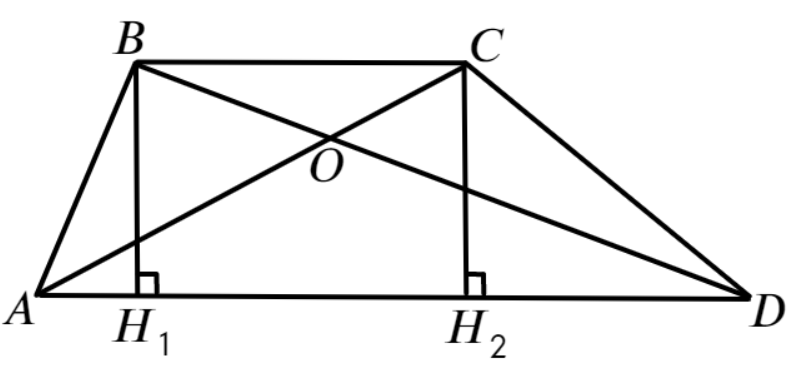
\includegraphics[scale=0.35]{g8-1.png}}
\end{figure}\\
Опустим высоты $BH_1$ и $CH_2.$ Тогда $BH_1H_2C$ является прямоугольником и $BH_1=CH_2.$ Поэтому $S_{\Delta ABD}=\cfrac{1}{2}BH_1\cdot AD=\cfrac{1}{2}CH_2\cdot AD=S_{\Delta ACD},$ значит $S_{\Delta AOB}=S_{\Delta ABD}-S_{\Delta AOD}=S_{\Delta ACD}-S_{\Delta AOD}=S_{\Delta COD},$ ч.т.д.\\
2. \begin{figure}[ht!]
\center{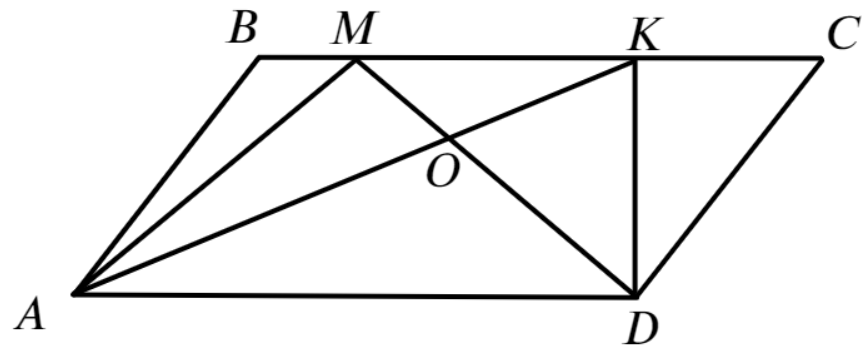
\includegraphics[scale=0.35]{g8-2.png}}
\end{figure}\\
Фигура $AMKD$ является трапецией, поэтому решение этой задачи полностью аналогично решению задачи 1.\\
3. \begin{figure}[ht!]
\center{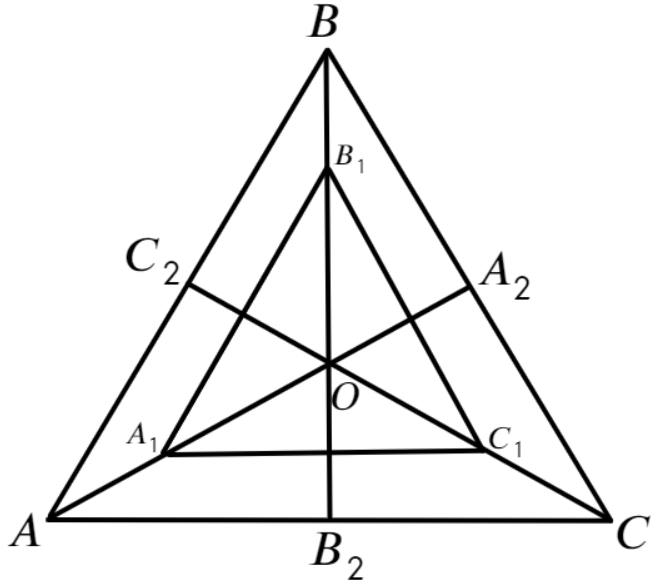
\includegraphics[scale=0.35]{g8-3.png}}
\end{figure}\\
Медианы делятся точкой пересечения в отношении $2:1,$ поэтому $AO=\cfrac{2}{3}AA_2.$ По условию $AA_1:A_1A_2=1:3,$ значит $AA_1=\cfrac{1}{4}AA_2.$ Тогда $A_1O=AO-AA_1=\cfrac{2}{3}AA_2-\cfrac{1}{4}AA_2=\cfrac{5}{12}AA_2.$ Таким образом,  $A_1O:AO=\cfrac{5}{12}AA_2:\cfrac{2}{3}AA_2=\cfrac{5}{8}$ и аналогично $B_1O:BO=C_1O:CO=\cfrac{5}{8}.$ Тогда треугольники $A_1B_1O$ с $ABO$ (а также $B_1C_1O$ с $BCO$ и $A_1C_1O$ с $ACO$) подобны по второму признаку (общий угол и одинаково относящиеся заключающие его стороны), коэффициент подобия равен $\cfrac{5}{8}.$ Тогда $S_{\Delta A_1B_1O}=\cfrac{25}{64}S_{\Delta ABO},\
S_{\Delta A_1C_1O}=\cfrac{25}{64}S_{\Delta ACO},\ S_{\Delta B_1C_1O}=\cfrac{25}{64}S_{\Delta BCO}\Rightarrow S_{\Delta A_1B_1C_1}=
S_{\Delta A_1B_1O}+S_{\Delta A_1C_1O}+S_{\Delta B_1C_1O}=\cfrac{25}{64}S_{\Delta ABO}+\cfrac{25}{64}S_{\Delta ACO}+\cfrac{25}{64}S_{\Delta BCO}=
\cfrac{25}{64}(S_{\Delta ABO}+S_{\Delta ACO}+S_{\Delta BCO})=\cfrac{25}{64}S_{\Delta ABC}.$
ewpage
oindent
4. \begin{figure}[ht!]
\center{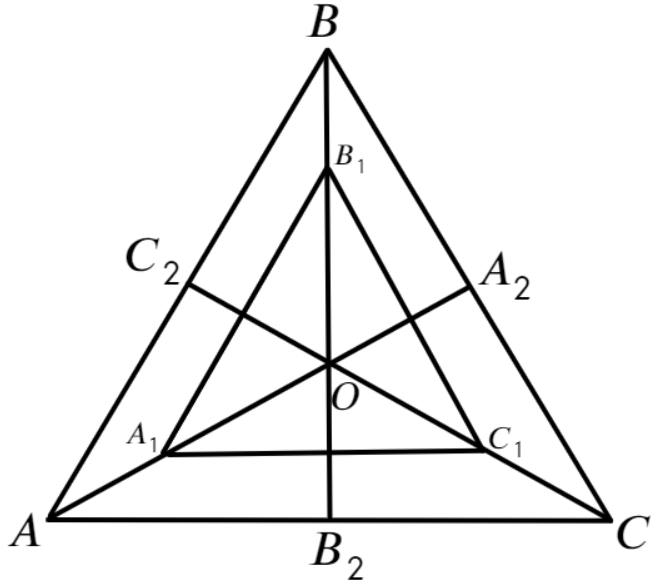
\includegraphics[scale=0.35]{g8-3.png}}
\end{figure}\\
Медианы делятся точкой пересечения в отношении $2:1,$ поэтому $AO=\cfrac{2}{3}AA_2.$ По условию $AA_1:A_1A_2=1:4,$ значит $AA_1=\cfrac{1}{5}AA_2.$ Тогда $A_1O=AO-AA_1=\cfrac{2}{3}AA_2-\cfrac{1}{5}AA_2=\cfrac{7}{15}AA_2.$ Таким образом,  $A_1O:AO=\cfrac{7}{15}AA_2:\cfrac{2}{3}AA_2=\cfrac{7}{10}$ и аналогично $B_1O:BO=C_1O:CO=\cfrac{7}{10}.$ Тогда треугольники $A_1B_1O$ с $ABO$ (а также $B_1C_1O$ с $BCO$ и $A_1C_1O$ с $ACO$) подобны по второму признаку (общий угол и одинаково относящиеся заключающие его стороны), коэффициент подобия равен $\cfrac{7}{10}.$ Тогда $S_{\Delta A_1B_1O}=\cfrac{49}{100}S_{\Delta ABO},\
S_{\Delta A_1C_1O}=\cfrac{49}{100}S_{\Delta ACO},\ S_{\Delta B_1C_1O}=\cfrac{49}{100}S_{\Delta BCO}\Rightarrow S_{\Delta A_1B_1C_1}=
S_{\Delta A_1B_1O}+S_{\Delta A_1C_1O}+S_{\Delta B_1C_1O}=\cfrac{49}{100}S_{\Delta ABO}+\cfrac{49}{100}S_{\Delta ACO}+\cfrac{49}{100}S_{\Delta BCO}=
\cfrac{49}{100}(S_{\Delta ABO}+S_{\Delta ACO}+S_{\Delta BCO})=\cfrac{49}{100}S_{\Delta ABC}.$\\
5. \begin{figure}[ht!]
\center{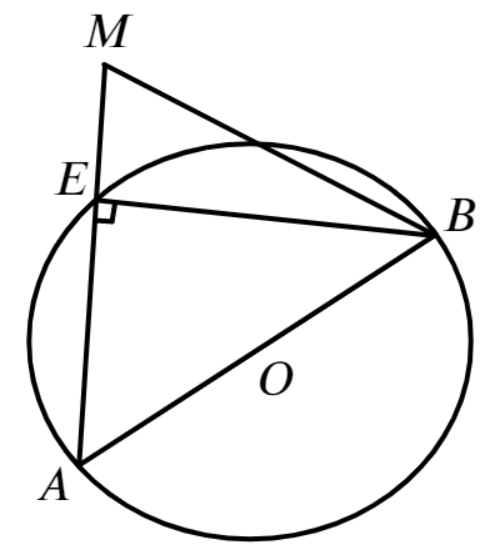
\includegraphics[scale=0.35]{g8-5.png}}
\end{figure}\\
В прямоугольном треугольнике медиана, проведённая из прямого угла, равна половине гипотенузы, значит $AB=2CM=24$см. Проведём высоту $CD,$ треугольники $ANH$ и $ACD$ подобны по двум углам (один прямой и один общий), значит $\cfrac{CD}{NH}=\cfrac{AC}{AN}=2,$ откуда $CD=2\cdot3=6$см. Тогда $S_{\Delta ABC}=\cfrac{1}{2} CD\cdot AB=\cfrac{1}{2}\cdot6\cdot24=72\text{ см}^2.$\\
6. \begin{figure}[ht!]
\center{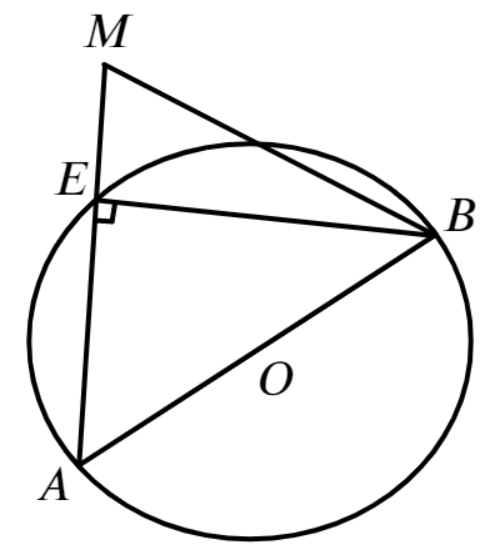
\includegraphics[scale=0.35]{g8-5.png}}
\end{figure}\\
В прямоугольном треугольнике медиана, проведённая из прямого угла, равна половине гипотенузы, значит $AB=2CM=16$см. Проведём высоту $CD,$ треугольники $ANH$ и $ACD$ подобны по двум углам (один прямой и один общий), значит $\cfrac{CD}{NH}=\cfrac{AC}{AN}=2,$ откуда $CD=2\cdot2=4$см. Тогда $S_{\Delta ABC}=\cfrac{1}{2} CD\cdot AB=\cfrac{1}{2}\cdot4\cdot16=32\text{ см}^2.$\\
7. \begin{figure}[ht!]
\center{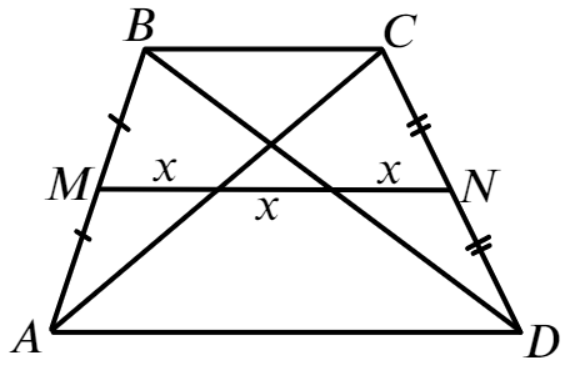
\includegraphics[scale=0.35]{g8-7.png}}
\end{figure}\\
Так как отрезок $MN$ является средней линией трапеции, он параллелен основаниям и проходит через середины $AB$ и $CD,$ а поэтому также содержит средние линии треугольников $ABC$ и $ABD.$ Тогда $x=\cfrac{1}{2}BD$ и $2x=\cfrac{1}{2}AD,$ откуда $BC=2x,\ AD=4x$ и $\cfrac{BC}{AD}=\cfrac{2x}{4x}=\cfrac{1}{2}.$\\
8. \begin{figure}[ht!]
\center{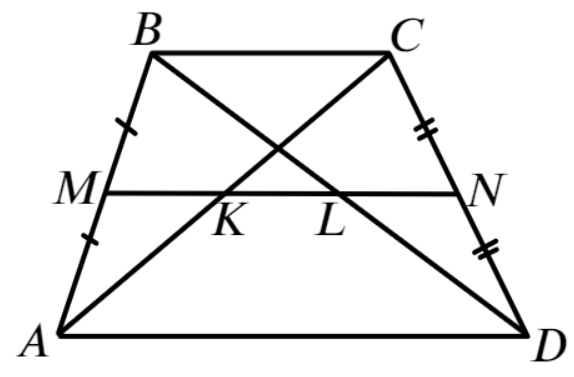
\includegraphics[scale=0.35]{g8-8.png}}
\end{figure}\\
Так как отрезок $MN$ является средней линией трапеции, он параллелен основаниям и проходит через середины $AB$ и $CD,$ а поэтому также содержит средние линии треугольников $ABC$ и $ACD,$ обозначим их $MK$ и $KN.$ Так как $MK+KN=8$см и $KN-MK=2$см, найдём $KN=5$см и $MK=3$см. Тогда $BC=2MK=6$см и $AD=2KN=10$см.\\
9. \begin{figure}[ht!]
\center{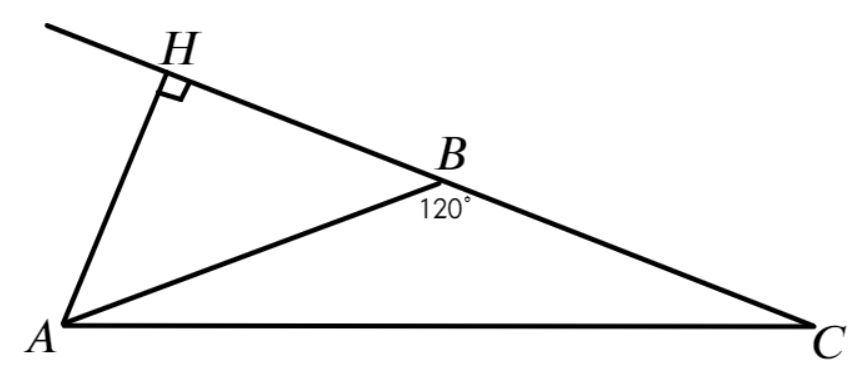
\includegraphics[scale=0.35]{g8-9.png}}
\end{figure}\\
Найдём $\angle C=\cfrac{1}{2}\left(180^\circ-120^\circ
ight)=30^\circ.$ Тогда в прямоугольном треугольнике $AHC$ катет $AH$ лежит напротив угла в $30^\circ,$ а значит равен половине гипотенузы $AC,$ поэтому $AC=2AH=2\cdot9=18$см.\\
10. \begin{figure}[ht!]
\center{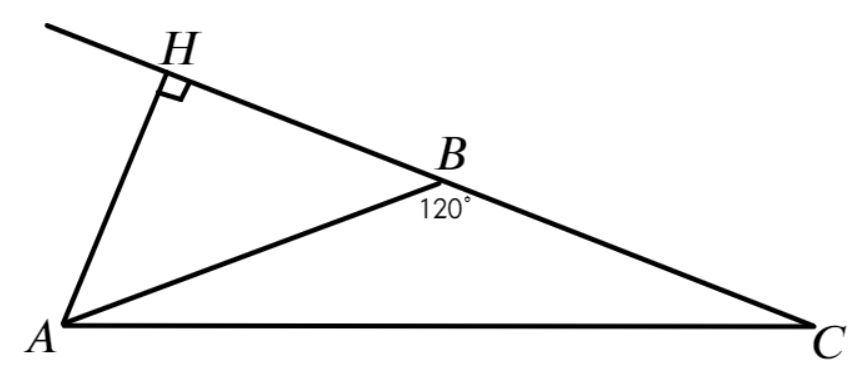
\includegraphics[scale=0.35]{g8-9.png}}
\end{figure}\\
Найдём $\angle C=\cfrac{1}{2}\left(180^\circ-120^\circ
ight)=30^\circ.$ Тогда в прямоугольном треугольнике $AHC$ катет $AH$ лежит напротив угла в $30^\circ,$ а значит равен половине гипотенузы $AC,$ поэтому $AH=\cfrac{1}{2}AC=\cfrac{1}{2}\cdot8=4$см.\\
11. \begin{figure}[ht!]
\center{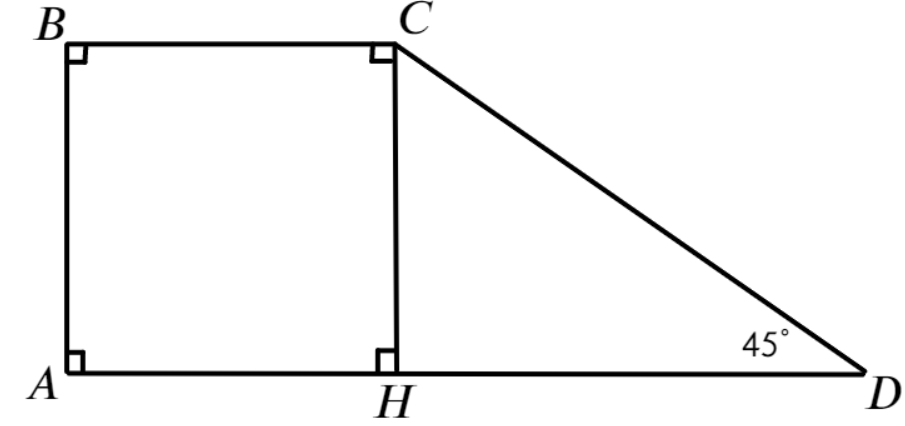
\includegraphics[scale=0.35]{g8-11.png}}
\end{figure}\\
Опустим из точки $C$ высоту $CH.$ Так как $AB=BC,$ четырёхугольник $ABCH$ является квадратом, поэтому $CH=AH=AB=6$ см. Найдём $\angle D=180^\circ-\angle C=180^\circ-135^\circ=45^\circ,$ поэтому $\angle HCD=180^\circ-90^\circ-45^\circ=45^\circ$ и треугольник $CHD$ является равнобедренным, $CH=HD.$ Тогда $AD=AH+HD=6+6=12$см и $S_{ABCD}=\cfrac{1}{2}\cdot6\cdot(6+12)=54\text{см}^2.$\\
12. \begin{figure}[ht!]
\center{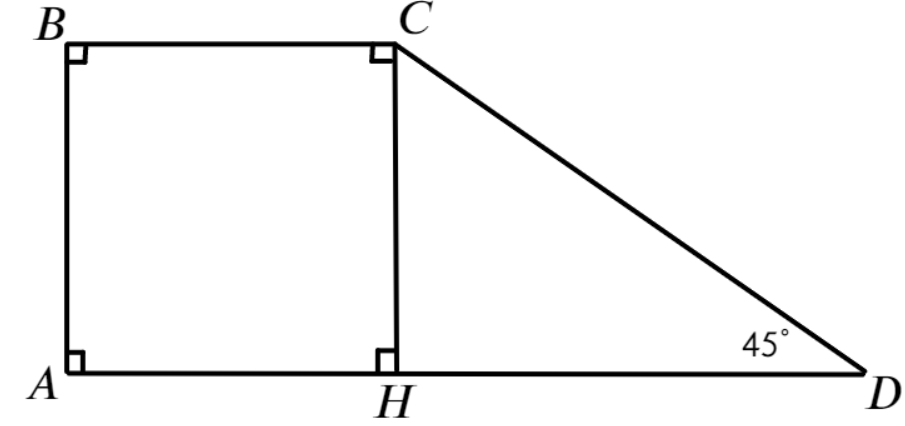
\includegraphics[scale=0.35]{g8-11.png}}
\end{figure}\\
Опустим из точки $C$ высоту $CH.$ Так как $AB=BC,$ четырёхугольник $ABCH$ является квадратом, поэтому $CH=AH=AB=4$ см. Найдём $\angle HCD=180^\circ-90^\circ-45^\circ=45^\circ$ и треугольник $CHD$ является равнобедренным, $CH=HD.$ Тогда $AD=AH+HD=4+4=8$см и $S_{ABCD}=\cfrac{1}{2}\cdot4\cdot(4+8)=24\text{см}^2.$\\
13. \begin{figure}[ht!]
\center{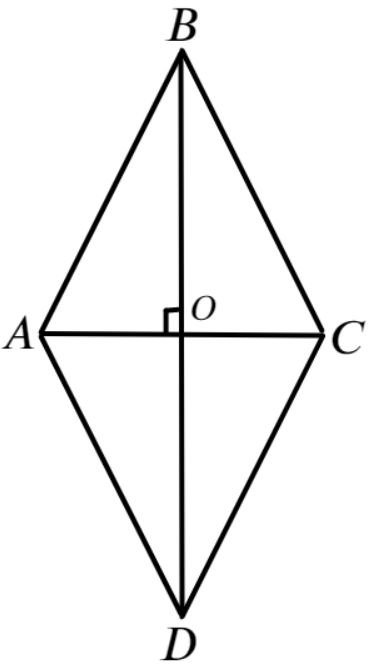
\includegraphics[scale=0.35]{g8-13.png}}
\end{figure}\\
Диагонали ромба перпендикулярны и делятся точкой пересечения пополам. Пусть $BO=\cfrac{1}{2}\cdot2\sqrt{3}=\sqrt{3}$ и $AO=\cfrac{1}{2}\cdot2=1.$ Тогда $tg(\angle ABO)=\cfrac{1}{\sqrt{3}}=\cfrac{\sqrt{3}}{3}\Rightarrow \angle ABO =30^\circ,\ \angle B=60^\circ,\ \angle D=\angle B=60^\circ,\ \angle A=\angle C=180^\circ-60^\circ=120^\circ.$
ewpage
oindent
14. \begin{figure}[ht!]
\center{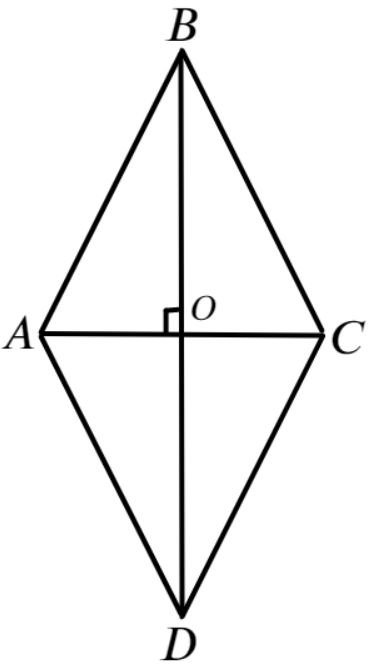
\includegraphics[scale=0.35]{g8-13.png}}
\end{figure}\\
Диагонали ромба перпендикулярны и делятся точкой пересечения пополам. Пусть $BO=\cfrac{1}{2}\cdot4\sqrt{3}=2\sqrt{3}$ и $AO=\cfrac{1}{2}\cdot4=2.$ Тогда $tg(\angle ABO)=\cfrac{2}{2\sqrt{3}}=\cfrac{\sqrt{3}}{3}\Rightarrow \angle ABO =30^\circ,\ \angle B=60^\circ,\ \angle D=\angle B=60^\circ,\ \angle A=\angle C=180^\circ-60^\circ=120^\circ.$\\
15. \begin{figure}[ht!]
\center{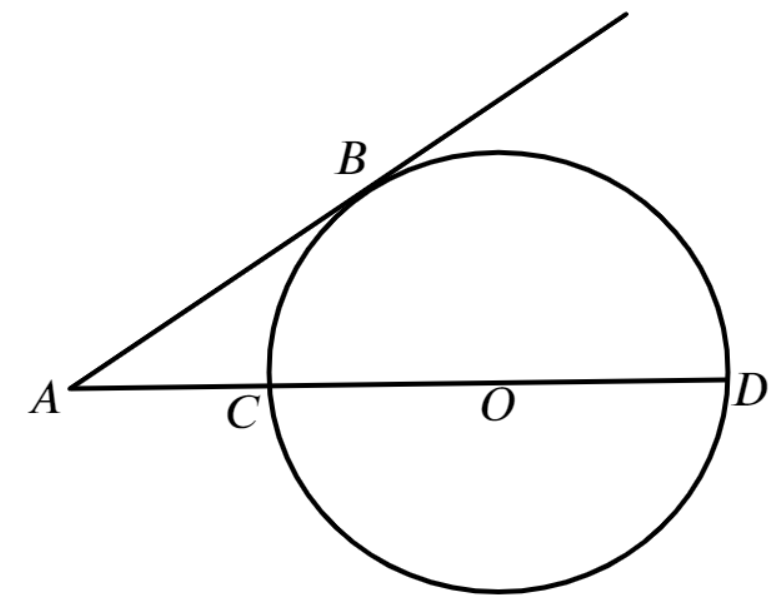
\includegraphics[scale=0.35]{g8-15.png}}
\end{figure}\\
По свойству касательной и секущей имеем $AB^2=AC\cdot AD.$ По условию $AD=2AB,$ значит $AB^2=AC\cdot2AB,\ AB=2AC.$ Пусть радиус окружности равен $x,$ тогда $AC=AD-2x,\ AC=2AB-2x,\ AC=4AC-2x,\ AC=\cfrac{2}{3}x.$ Поэтому $AB=2AC=\cfrac{4}{3}x.$\\
16. \begin{figure}[ht!]
\center{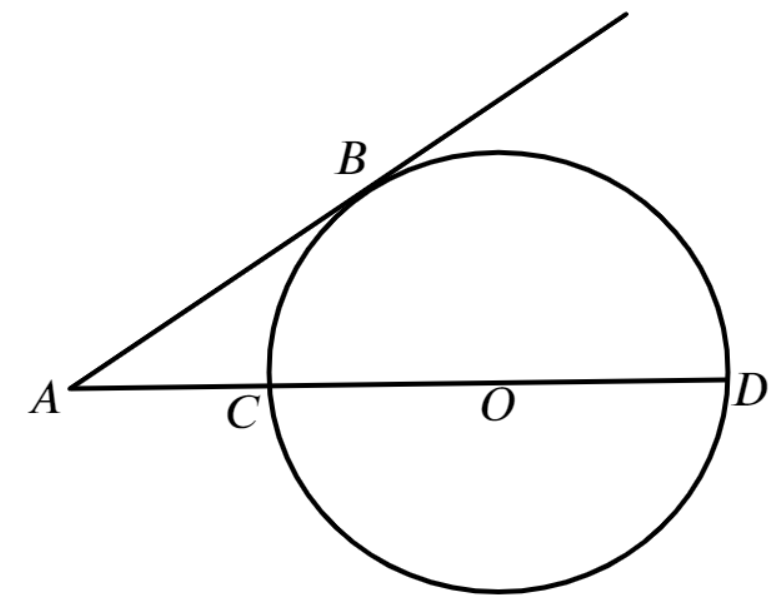
\includegraphics[scale=0.35]{g8-15.png}}
\end{figure}\\
По свойству касательной и секущей имеем $AB^2=AC\cdot AD.$ По условию $AD=3AB,$ значит $AB^2=AC\cdot3AB,\ AB=3AC.$ Пусть радиус окружности равен $x,$ тогда $AC=AD-2x,\ AC=3AB-2x,\ AC=9AC-2x,\ AC=\cfrac{1}{4}x.$ Поэтому $AB=3AC=\cfrac{3}{4}x,$ значит $x=\cfrac{4}{3}AB.$
ewpage
oindent
17. \begin{figure}[ht!]
\center{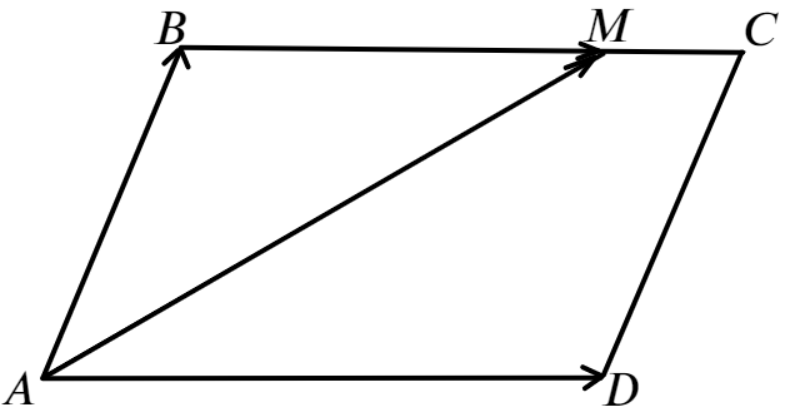
\includegraphics[scale=0.35]{g8-17.png}}
\end{figure}\\
$\overrightarrow{AM}=\overrightarrow{AB}+\overrightarrow{BM}=\overrightarrow{AB}+\cfrac{3}{4}\overrightarrow{BC}=
\overrightarrow{AB}+\cfrac{3}{4}\overrightarrow{AD}.$\\
18. \begin{figure}[ht!]
\center{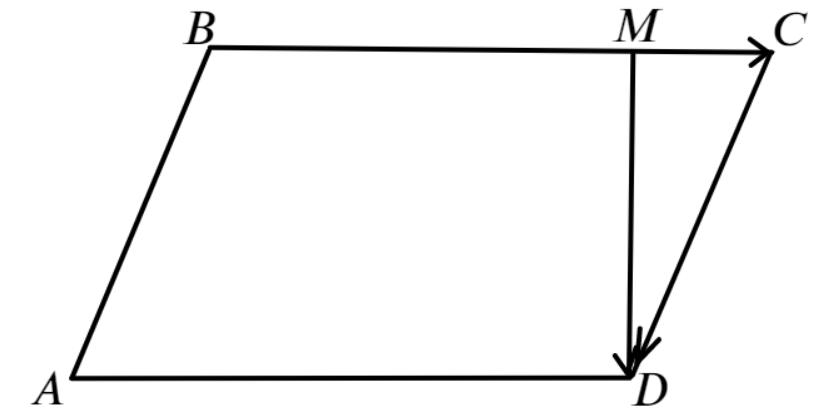
\includegraphics[scale=0.35]{g8-18.png}}
\end{figure}\\
$\overrightarrow{MD}=\overrightarrow{MC}+\overrightarrow{CD}=\cfrac{1}{4}\overrightarrow{BC}-\overrightarrow{AB}=
\cfrac{1}{4}\overrightarrow{AD}-\overrightarrow{AB}.$\\
19. \begin{figure}[ht!]
\center{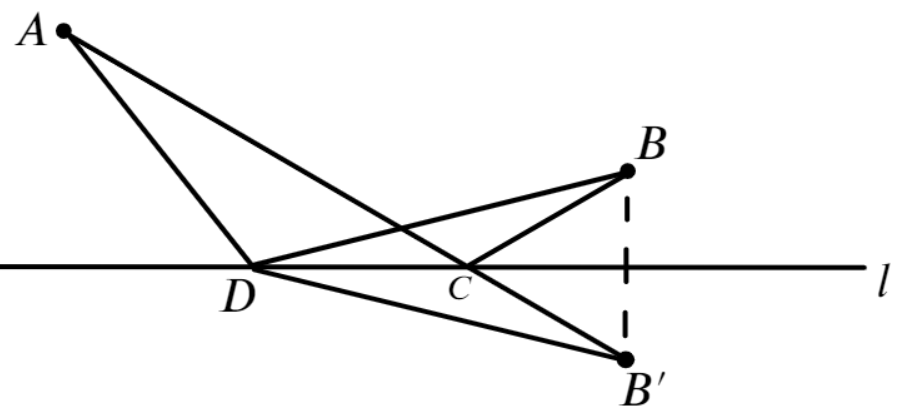
\includegraphics[scale=0.35]{g8-19.png}}
\end{figure}\\
Отразим точку $B$ симметрично относительно прямой $l,$ получим точку $B'.$ Пусть прямая $AB'$ пересекает прямую $l$ в точке $C.$ Докажем, что именно эта точка будет искомой. Возьмём на прямой $l$ другую точку $D.$ Тогда $AC+BC=AC+B'C=AB'<AD+B'D\text{ (по неравенству треугольника) }=AD+BD.$\\
20. \begin{figure}[ht!]
\center{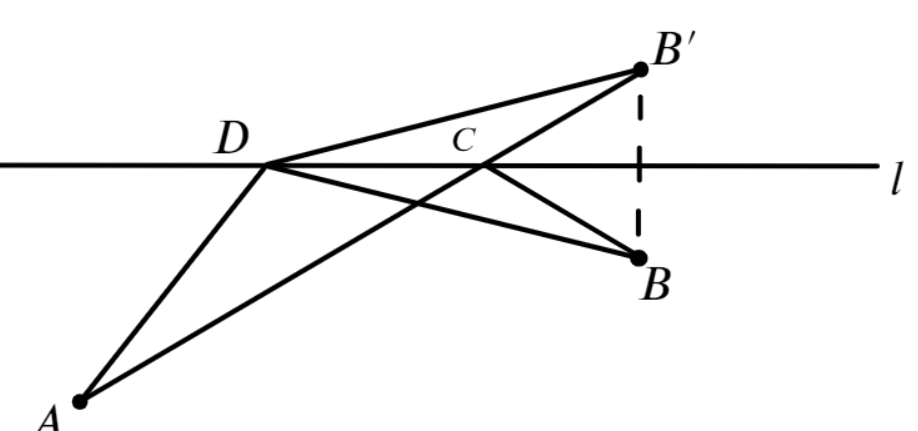
\includegraphics[scale=0.35]{g8-20.png}}
\end{figure}\\
Отразим точку $B$ симметрично относительно прямой $l,$ получим точку $B'.$ Пусть прямая $AB'$ пересекает прямую $l$ в точке $C.$ Докажем, что именно эта точка будет искомой. Возьмём на прямой $l$ другую точку $D.$ Тогда $AC+BC=AC+B'C=AB'<AD+B'D\text{ (по неравенству треугольника) }=AD+BD.$
ewpage
oindent
21. \begin{figure}[ht!]
\center{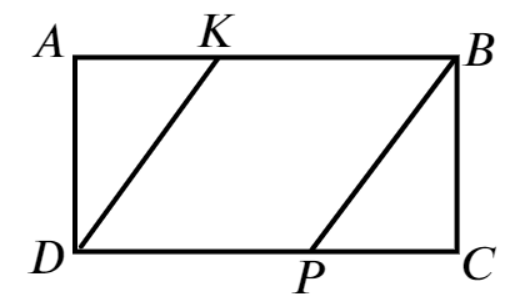
\includegraphics[scale=0.35]{g8-21.png}}
\end{figure}\\
$AK=\cfrac{3}{8}AB=\cfrac{3}{8}\cdot8=3\Rightarrow KB=8-3=5,$ аналогично $DP=5,$ значит в четырёхугольнике $KBPD$ противоположные стороны параллельны и равны, поэтому он является параллелограммом. Также по теореме Пифагора $KD=\sqrt{AK^2+AD^2}=\sqrt{9+16}=5,$ аналогично $BP=5,$ поэтому $KBPD$ является ромбом. Его периметр равен $4\cdot5=20,$ а площадь равна $BC\cdot DP=4\cdot5=20.$\\
22. \begin{figure}[ht!]
\center{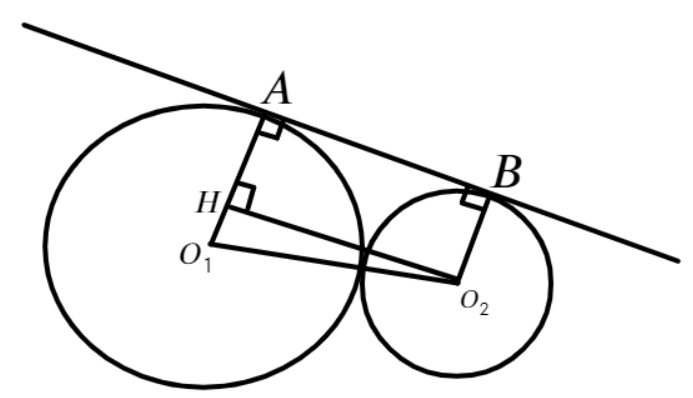
\includegraphics[scale=0.35]{g8-22.png}}
\end{figure}\\
Радиусы, проведённые к точке касания, перпендикулярны касательной, поэтому $O_1ABO_2$ является прямоугольной трапецией. Точка касания двух окружностей лежит на одной прямой с их центрами, поэтому $O_1O_2=8+2=10.$ Проведём высоту $O_2H,$ тогда $HABO_2$ является прямоугольником и $AH=O_2B=2,$ тогда $O_1H=O_1A-AH=8-2=6.$ По теореме Пифагора $O_2H=\sqrt{O_1O_2^2-O_1H^2}=\sqrt{10^2-6^2}=8,$ тогда $AB=O_2H=8.$\\
23. \begin{figure}[ht!]
\center{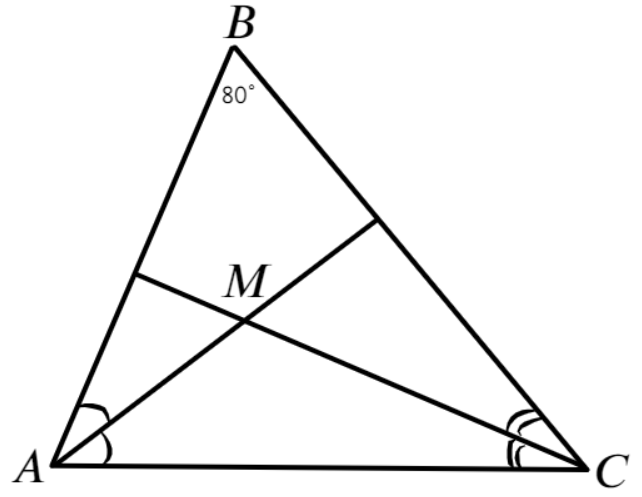
\includegraphics[scale=0.35]{g8-23.png}}
\end{figure}\\
$\angle AMC=180^\circ-\angle MAC-\angle MCA=180^\circ-\cfrac{1}{2}\angle A-\cfrac{1}{2}\angle C=180^\circ-\cfrac{1}{2}(\angle A+\angle C)=
180^\circ-\cfrac{1}{2}(180^\circ-80^\circ)=130^\circ.$\\
24. \begin{figure}[ht!]
\center{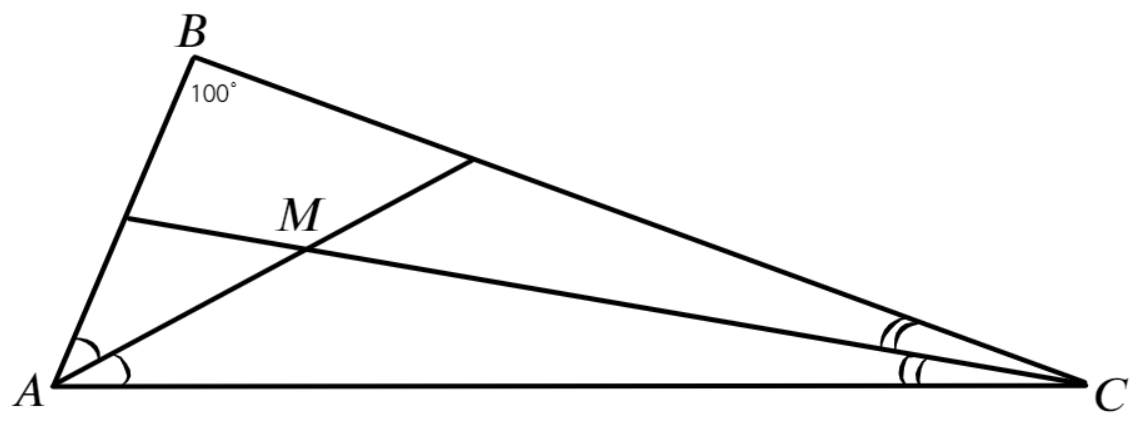
\includegraphics[scale=0.35]{g8-24.png}}
\end{figure}\\
$\angle AMC=180^\circ-\angle MAC-\angle MCA=180^\circ-\cfrac{1}{2}\angle A-\cfrac{1}{2}\angle C=180^\circ-\cfrac{1}{2}(\angle A+\angle C)=
180^\circ-\cfrac{1}{2}(180^\circ-100^\circ)=140^\circ.$\\
25. $S=\cfrac{1}{2}d_1d_2.$ Если $d_1=1,5d_2,$ то $27=\cfrac{1}{2}\cdot1,5d_2\cdot d_2,\ d_2^2=36,\ d_2=6$см, а $d_1=1,5\cdot6=9$см.\\
26. $S=\cfrac{1}{2}d_1d_2.$ Если $d_1=2,5d_2,$ то $20=\cfrac{1}{2}\cdot2,5d_2\cdot d_2,\ d_2^2=16,\ d_2=4$см, а $d_1=2,5\cdot4=10$см.\\
27. \begin{figure}[ht!]
\center{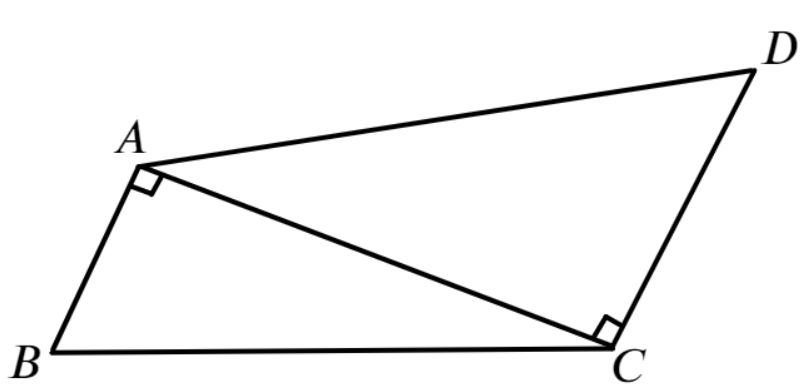
\includegraphics[scale=0.35]{g8-27.png}}
\end{figure}\\
Так как $5^2+12^2=13^2$ и $9^2+12^2=15^2,$ по обратной теореме Пифагора треугольники $ABC$ и $CAD$ являются прямоугольными. Тогда $S_{ABCD}=S_{ABC}+S_{CAD}=\cfrac{1}{2}\cdot5\cdot12+\cfrac{1}{2}\cdot9\cdot12=84.$\\
28. \begin{figure}[ht!]
\center{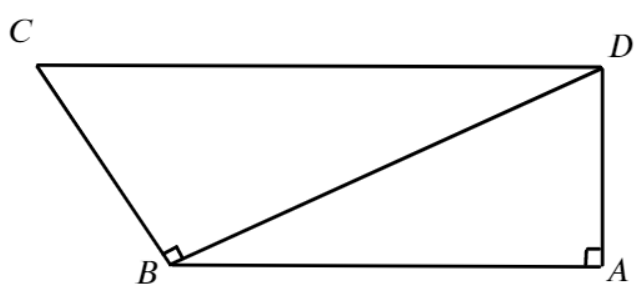
\includegraphics[scale=0.35]{g8-28.png}}
\end{figure}\\
Так как $8^2+15^2=17^2$ и $9^2+12^2=15^2,$ по обратной теореме Пифагора треугольники $BCD$ и $BAD$ являются прямоугольными. Тогда $S_{ABCD}=S_{BCD}+S_{BAD}=\cfrac{1}{2}\cdot8\cdot15+\cfrac{1}{2}\cdot9\cdot12=114.$\\
29. \begin{figure}[ht!]
\center{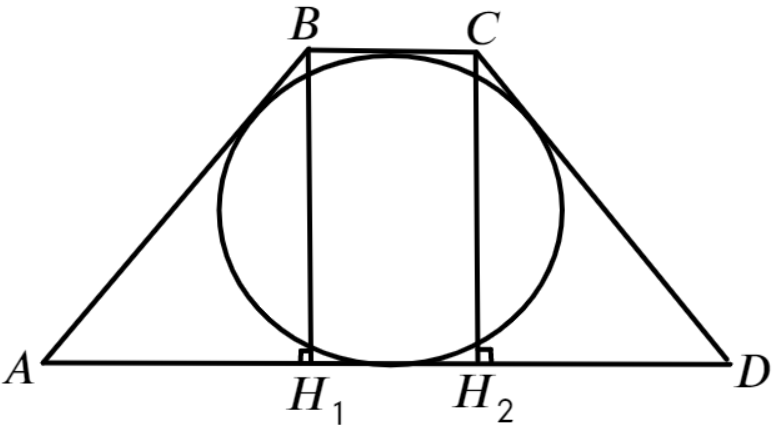
\includegraphics[scale=0.35]{g8-29.png}}
\end{figure}\\
Так как трапеция является описанным четырёхугольником, суммы его противоположных сторон равны. Так как она равнобедренная, $2AB=2CD=BC+AD=36+100=136,\ AB=CD=68$см. Опустим две высоты $BH_1$ и $CH_2,$ тогда $H_1H_2=BC=36$см, $AH_1=DH_2=(100-36):2=32$см. По теореме Пифагора $BH_1=\sqrt{68^2-32^2}=60$см. Тогда $R=BH_1:2=60:2=30$см.\\
30. \begin{figure}[ht!]
\center{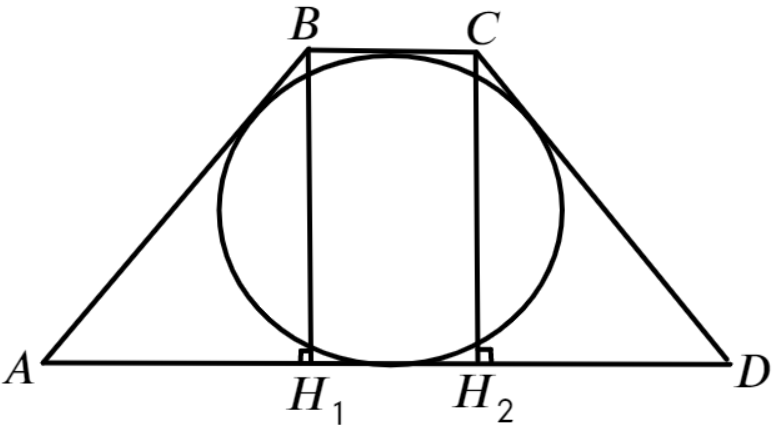
\includegraphics[scale=0.35]{g8-29.png}}
\end{figure}\\
Так как трапеция является описанным четырёхугольником, суммы его противоположных сторон равны. Так как она равнобедренная, $2AB=2CD=BC+AD=32+50=82,\ AB=CD=41$см. Опустим две высоты $BH_1$ и $CH_2,$ тогда $H_1H_2=BC=32$см, $AH_1=DH_2=(50-32):2=9$см. По теореме Пифагора $BH_1=\sqrt{41^2-9^2}=40$см. Тогда $R=BH_1:2=40:2=20$см.
ewpage
oindent
31. По свойству об отрезках хорды если вторая хорда поделилась на две части по $x$см, то $48\cdot3=x\cdot x,\ x^2=144,\ x=12$см. Значит, длина второй хорды равна $12\cdot2=24$см.\\
32. По свойству об отрезках хорды если вторая хорда поделилась на две части по $x$см, то $16\cdot4=x\cdot x,\ x^2=64,\ x=8$см. Значит, длина второй хорды равна $8\cdot2=16$см.\\
33. Возможны два случая: углы треугольника равны $2x,\ 2x$ и $5x$ или $5x,\ 5x$ и $2x.$ Тогда либо $2x+2x+5x=180^\circ,\ 9x=180^\circ,\ x=20^\circ$ и углы равны
$40^\circ,\ 40^\circ$  и $100^\circ,$ либо $5x+5x+2x=180^\circ,\ 12x=180^\circ,\ x=15^\circ$ и углы равны $75^\circ,\ 75^\circ$ и $30^\circ.$\\
34. Возможны два случая: углы треугольника равны $x,\ x$ и $4x$ или $4x,\ 4x$ и $x.$ Тогда либо $x+x+4x=180^\circ,\ 6x=180^\circ,\ x=30^\circ$ и углы равны
$30^\circ,\ 30^\circ$  и $120^\circ,$ либо $4x+4x+x=180^\circ,\ 9x=180^\circ,\ x=20^\circ$ и углы равны $80^\circ,\ 80^\circ$ и $20^\circ.$\\
35. Для того, чтобы выполнялись неравенства треугольника, третья сторона должна быть равна как минимум $4-2+1=3$ и как максимум $4+2-1=5.$ Значит, её значение может быть равно 3, 4 или 5.\\
36. Для того, чтобы выполнялись неравенства треугольника, третья сторона должна быть равна как минимум $5-2+1=4$ и как максимум $5+2-1=6.$ Значит, её значение может быть равно 4, 5 или 6.\\
37. \begin{figure}[ht!]
\center{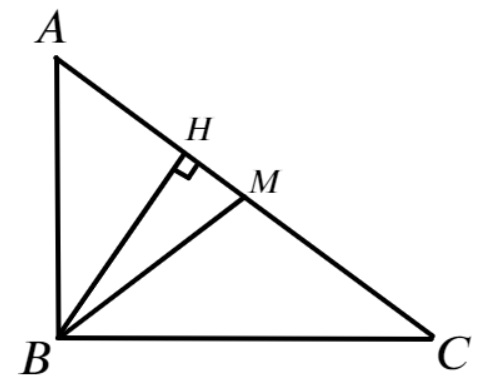
\includegraphics[scale=0.35]{g8-37.png}}
\end{figure}\\
Проведём медиану $BM,$ она равна половине гипотенузы $10:2=5$см. Проведём высоту $BH,$ она либо совпадает с медианой, либо меньше её как катет в прямоугольном треугольнике $BHM.$ Тогда $S=\cfrac{1}{2}\cdot BH\cdot AC\leqslant  \cfrac{1}{2}\cdot BM \cdot AC=\cfrac{1}{2}\cdot 5\cdot 10=25\text{ см}^2.$\\
38. \begin{figure}[ht!]
\center{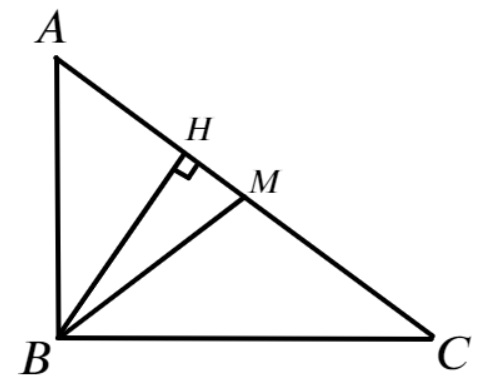
\includegraphics[scale=0.35]{g8-37.png}}
\end{figure}\\
Проведём медиану $BM,$ она равна половине гипотенузы $12:2=6$см. Проведём высоту $BH,$ она либо совпадает с медианой, либо меньше её как катет в прямоугольном треугольнике $BHM.$ Тогда $S=\cfrac{1}{2}\cdot BH\cdot AC\leqslant  \cfrac{1}{2}\cdot BM \cdot AC=\cfrac{1}{2}\cdot 6\cdot 12=36\text{ см}^2.$\\
39. Возможны два случая: углы треугольника равны $x,\ x$ и $4x$ или $4x,\ 4x$ и $x.$ Тогда либо $x+x+4x=180^\circ,\ 6x=180^\circ,\ x=30^\circ$ и углы треугольника равны $30^\circ,\ 30^\circ$  и $120^\circ,$ либо $4x+4x+x=180^\circ,\ 9x=180^\circ,\ x=20^\circ$ и углы треугольника равны $80^\circ,\ 80^\circ$ и $20^\circ.$ В первом случае у параллелограмма будет два угла по $30^\circ$ и два угла по $180^\circ-30^\circ=150^\circ.$ Во втором случае у параллелограмма будет два угла по $80^\circ$ и два угла по $180^\circ-80^\circ=100^\circ.$\\
40. Возможны два случая: углы треугольника равны $2x,\ 2x$ и $5x$ или $5x,\ 5x$ и $2x.$ Тогда либо $2x+2x+5x=180^\circ,\ 9x=180^\circ,\ x=20^\circ$ и углы треугольника равны $40^\circ,\ 40^\circ$  и $100^\circ,$ либо $5x+5x+2x=180^\circ,\ 12x=180^\circ,\ x=15^\circ$ и углы треугольника равны $75^\circ,\ 75^\circ$ и $30^\circ.$ В первом случае у параллелограмма будет два угла по $40^\circ$ и два угла по $180^\circ-40^\circ=140^\circ.$ Во втором случае у параллелограмма будет два угла по $75^\circ$ и два угла по $180^\circ-75^\circ=105^\circ.$
ewpage
oindent
41. \begin{figure}[ht!]
\center{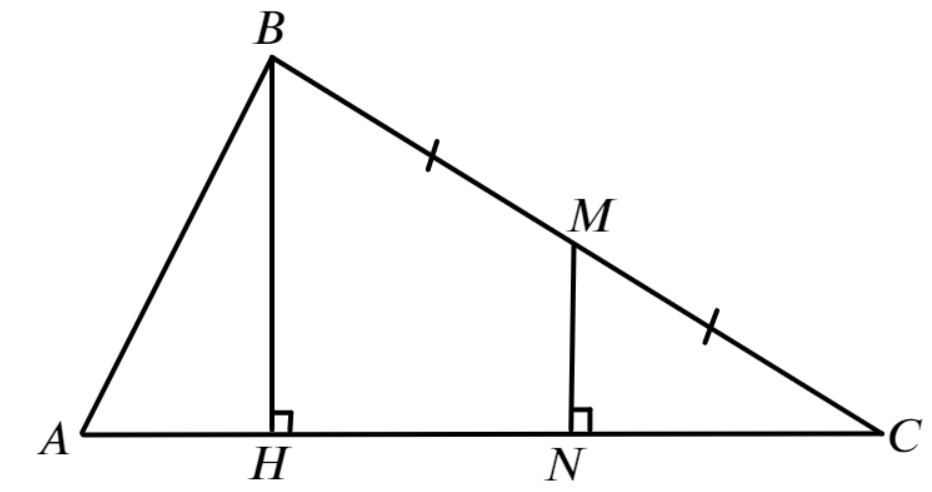
\includegraphics[scale=0.35]{g8-41.png}}
\end{figure}\\
По теореме Пифагора $MN=\sqrt{MC^2-NC^2}=\sqrt{289-225}=8$см. Проведём высоту $BH.$ Треугольники $BHC$ и $MNC$ подобны по двум углам (прямой и общий угол $C$), поэтому $\cfrac{BH}{MN}=\cfrac{BC}{MC}=2\Rightarrow BH=2\cdot8=16$см. Тогда $S_{\Delta ABC}=\cfrac{1}{2}BH\cdot AC=\cfrac{1}{2}\cdot16\cdot(25+15)=320\text{ см}^2.$\\
42. \begin{figure}[ht!]
\center{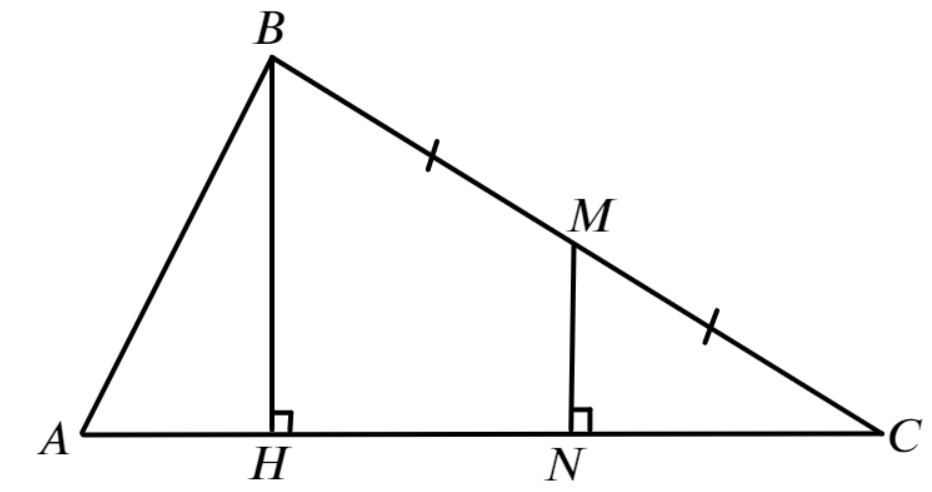
\includegraphics[scale=0.35]{g8-41.png}}
\end{figure}\\
По теореме Пифагора $MN=\sqrt{MC^2-NC^2}=\sqrt{169-25}=12$см. Проведём высоту $BH.$ Треугольники $BHC$ и $MNC$ подобны по двум углам (прямой и общий угол $C$), поэтому $\cfrac{BH}{MN}=\cfrac{BC}{MC}=2\Rightarrow BH=2\cdot12=24$см. Тогда $S_{\Delta ABC}=\cfrac{1}{2}BH\cdot AC=\cfrac{1}{2}\cdot24\cdot(19+5)=288\text{ см}^2.$\\
43. \begin{figure}[ht!]
\center{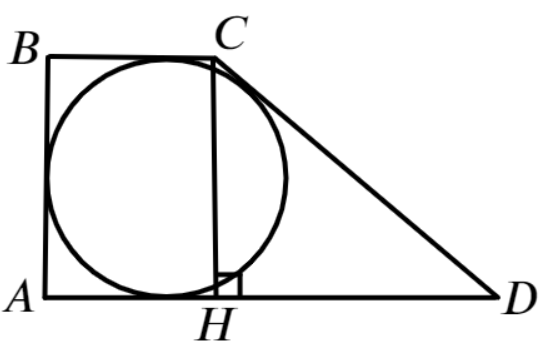
\includegraphics[scale=0.35]{g8-43.png}}
\end{figure}\\
Так как трапеция является описанным четырёхугольником, суммы её противоположных сторон равны. Проведём высоту $CH,$ тогда $HD=AD-AH=AD-BC=6-4=2,$ $CH=AB.$ Пусть $AB=x,$ тогда $AB+CD=BC+AD,\ CD=BC+AD-AB=4+6-x=10-x.$ По теореме Пифагора для треугольника $CHD$ имеем $x^2+2^2=(10-x)^2,\ x^2+4=100-20x+x^2,\ x=4,8$см. Тогда $R=\cfrac{1}{2}\cdot CH=\cfrac{1}{2}\cdot 4,8=2,4$см.\\
44. \begin{figure}[ht!]
\center{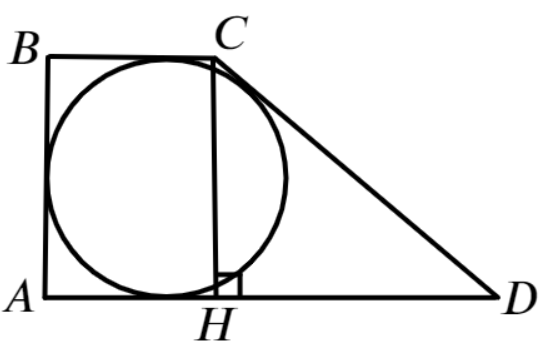
\includegraphics[scale=0.35]{g8-43.png}}
\end{figure}\\
Так как трапеция является описанным четырёхугольником, суммы её противоположных сторон равны. Проведём высоту $CH,$ тогда $HD=AD-AH=AD-BC=3-2=1,$ $CH=AB.$ Пусть $AB=x,$ тогда $AB+CD=BC+AD,\ CD=BC+AD-AB=3+2-x=5-x.$ По теореме Пифагора для треугольника $CHD$ имеем $x^2+1^2=(5-x)^2,\ x^2+1=25-10x+x^2,\ x=2,4$см. Тогда $R=\cfrac{1}{2}\cdot CH=\cfrac{1}{2}\cdot 2,4=1,2$см.\\
45. Координаты точки $M$ равны $\left(\cfrac{2+4}{2};\cfrac{-5-3}{2}
ight)=(3;-4).$ Тогда $|CM|=\sqrt{(3-0)^2+(-4-0)^2}=5.$\\
46. Координаты точки $M$ равны $\left(\cfrac{-2-4}{2};\cfrac{5+3}{2}
ight)=(-3;4).$ Тогда $|CM|=\sqrt{(-3-0)^2+(4-0)^2}=5.$\\
47. \begin{figure}[ht!]
\center{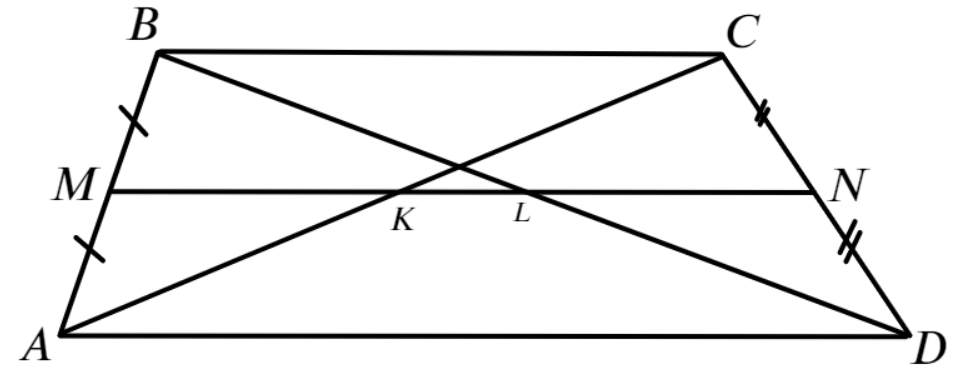
\includegraphics[scale=0.35]{g8-47.png}}
\end{figure}\\
Так как средняя линии трапеции $MN$ параллельна основаниям трапеции и проходит через середины $AB$ и $CD,$ отрезки $MK,\ KN$ и $LN$ также являются средними линиями в соответствующих треугольниках. Тогда $MN=\cfrac{1}{2}(12+18)=15$см, $MK=LN=\cfrac{1}{2}\cdot12=6$см, $KL=15-6-6=3$см.\\
48. \begin{figure}[ht!]
\center{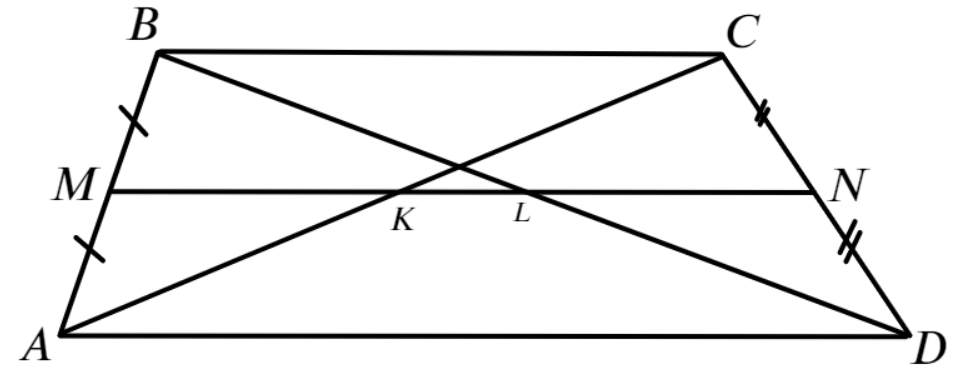
\includegraphics[scale=0.35]{g8-47.png}}
\end{figure}\\
Так как средняя линии трапеции $MN$ параллельна основаниям трапеции и проходит через середины $AB$ и $CD,$ отрезки $MK,\ KN$ и $LN$ также являются средними линиями в соответствующих треугольниках. Тогда $MN=\cfrac{1}{2}(10+16)=13$см, $MK=LN=\cfrac{1}{2}\cdot10=5$см, $KL=13-5-5=3$см.\\
49. \begin{figure}[ht!]
\center{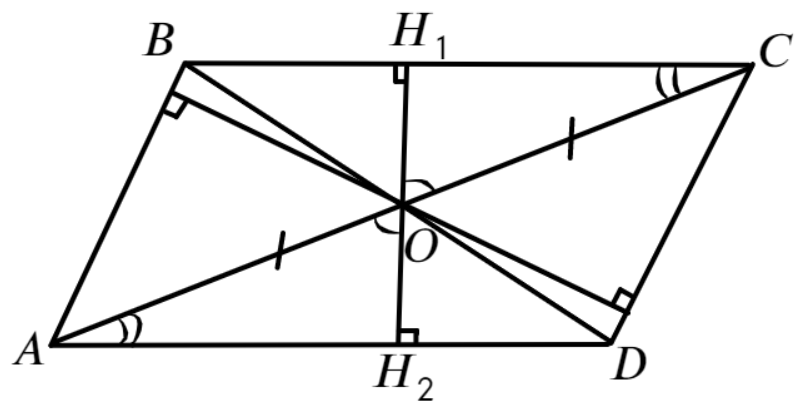
\includegraphics[scale=0.35]{g8-49.png}}
\end{figure}\\
Проведём перпендикуляры из точки пересечения диагоналей ко всем сторонам параллелограмма. Треугольники $AOH_2$ и $COH_1$ равны по второму признаку: $AO=OC,$ Углы $AOH_2$ и $COH_1$ вертикальные, а $H_2AO$ и $H_1CO$ --- накрест лежащие. Значит, $H_1O=H_2O,$ поэтому $H_1H_2=2OH_1.$ Поэтому высоты параллелограмма в два раза больше, чем расстояния от точки пересечения диагоналей до сторон. Тогда одна сторона равна $24:6=4$см, а другая $24:4=6$см, таким образом периметр параллелограмма равен $(4+6)\cdot2=20$см.\\
50. \begin{figure}[ht!]
\center{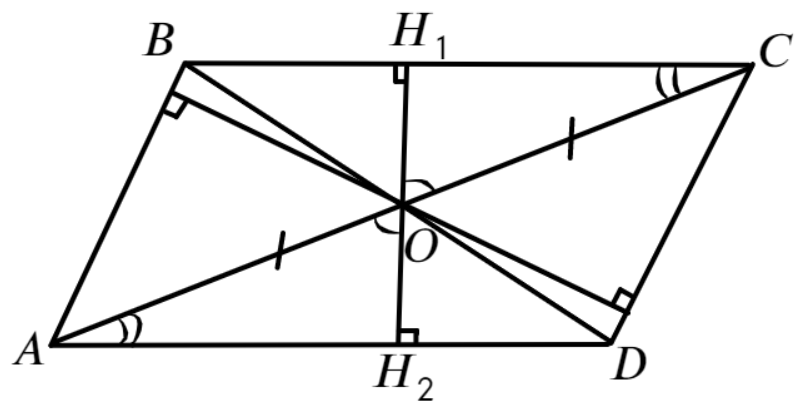
\includegraphics[scale=0.35]{g8-49.png}}
\end{figure}\\
Проведём перпендикуляры из точки пересечения диагоналей ко всем сторонам параллелограмма. Треугольники $AOH_2$ и $COH_1$ равны по второму признаку: $AO=OC,$ Углы $AOH_2$ и $COH_1$ вертикальные, а $H_2AO$ и $H_1CO$ --- накрест лежащие. Значит, $H_1O=H_2O,$ поэтому $H_1H_2=2OH_1.$ Поэтому высоты параллелограмма в два раза больше, чем расстояния от точки пересечения диагоналей до сторон. Тогда одна сторона равна $48:6=8$см, а другая $48:8=6$см, таким образом периметр параллелограмма равен $(8+6)\cdot2=28$см.\\
51. \begin{figure}[ht!]
\center{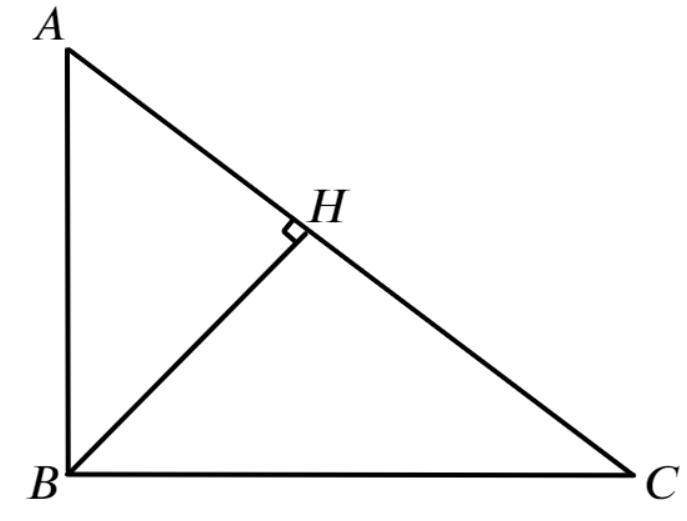
\includegraphics[scale=0.35]{g8-51.png}}
\end{figure}\\
Пусть катеты прямоугольного треугольник равны $3x$ и $4x,$ тогда по теореме Пифагора $9x^2+16x^2=2500,\ x^2=100,\ x=10.$ Тогда площадь треугольника $ABC$ с одной стороны равна $\cfrac{1}{2}\cdot30\cdot40=600,$ а с другой стороны равна $\cfrac{1}{2}BH\cdot50=25BH,$ значит $BH=600:25=24.$ По теореме Пифагора для треугольника $ABH$ имеем $AH=\sqrt{900-576}=18,$ тогда $HC=50-18=32.$\\
52. \begin{figure}[ht!]
\center{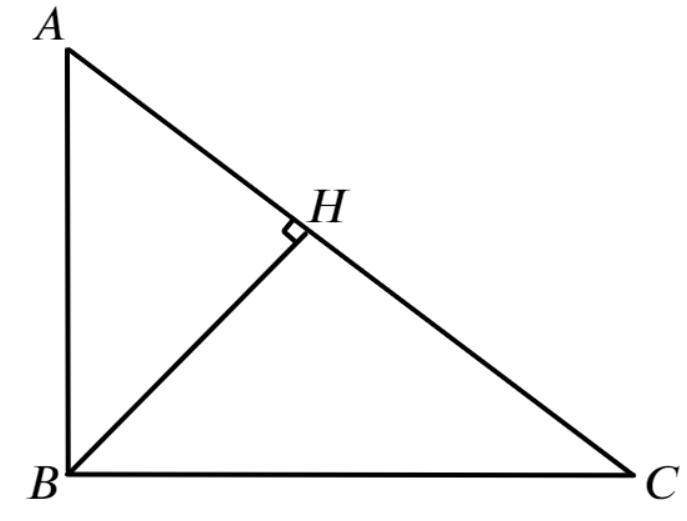
\includegraphics[scale=0.35]{g8-51.png}}
\end{figure}\\
Пусть $AB:AC=3:5,$ тогда $AB=25:5\cdot3=15$см. По теореме Пифагора $BC=\sqrt{625-225}=20$см. Тогда площадь треугольника $ABC$ с одной стороны равна $\cfrac{1}{2}\cdot15\cdot20=150\text{ см}^2,$ а с другой стороны равна $\cfrac{1}{2}BH\cdot25=12,5BH,$ значит $BH=150:12,5=12$см. По теореме Пифагора для треугольника $ABH$ имеем $AH=\sqrt{225-144}=9$см, тогда $HC=25-9=16$см.\\
53. Заметим, что $12^2+5^2=13^2.$ Значит, по обратной теореме Пифагора этот треугольник является прямоугольным. Наибольшей его стороной является гипотенуза 13 см, а проведённая к ней медиана равна её половине $13:2=6,5$см.\\
54. Заметим, что $8^2+6^2=10^2.$ Значит, по обратной теореме Пифагора этот треугольник является прямоугольным. Наибольшей его стороной является гипотенуза 10 см, а проведённая к ней медиана равна её половине $10:2=5$см.\\
55. Если $tg A=\cfrac{1}{2},$ то $BC=x,\ AC=2x.$ Тогда по теореме Пифагора $AB=\sqrt{x^2+4x^2}=\sqrt{5}x.$ Поэтому $\cos A=\cfrac{2x}{\sqrt{5}x}=\cfrac{2\sqrt{5}}{5}.$\\
56. Если $tg A=\cfrac{1}{2},$ то $BC=2x,\ AC=3x.$ Тогда по теореме Пифагора $AB=\sqrt{4x^2+9x^2}=\sqrt{13}x.$ Поэтому $\cos A=\cfrac{3x}{\sqrt{13}x}=\cfrac{3\sqrt{13}}{13}.$\\
57. Пусть стороны параллелограмма равны $a$ и $b,$ а проведённые к ним высоты --- $h$ и $2h.$ Тогда $S=a\cdot h=b\cdot 2h\Rightarrow a=2b$ и $(a+b)\cdot2=18,\ 3b=9,\ b=3$см. Значит, стороны параллелограмма равны 3 см и $3\cdot2=6$см.\\
58. Пусть стороны равны $a$ и $b,$ тогда $\begin{cases}(a+b)\cdot2=28,\\ a^2+b^2=10^2.\end{cases}\Leftrightarrow
\begin{cases}b=14-a,\\ a^2+(14-a)^2=100.\end{cases}\Leftrightarrow$\\$
\begin{cases}b=14-a,\\ 2a^2-28a+96=0.\end{cases}\Leftrightarrow
\left[\begin{array}{l}\begin{cases}a=6\text{ см},\\ b=8\text{ см}.\end{cases}\\ \begin{cases}a=8\text{ см},\\ b=6\text{ см}.\end{cases}\end{array}
ight.$\\
59. $(n-2)\cdot180^\circ=2\cdot360^\circ,\ n-2=4,\ n=6.$\\
60. $(n-2)\cdot180^\circ=3\cdot360^\circ,\ n-2=6,\ n=8.$\\
61. \begin{figure}[ht!]
\center{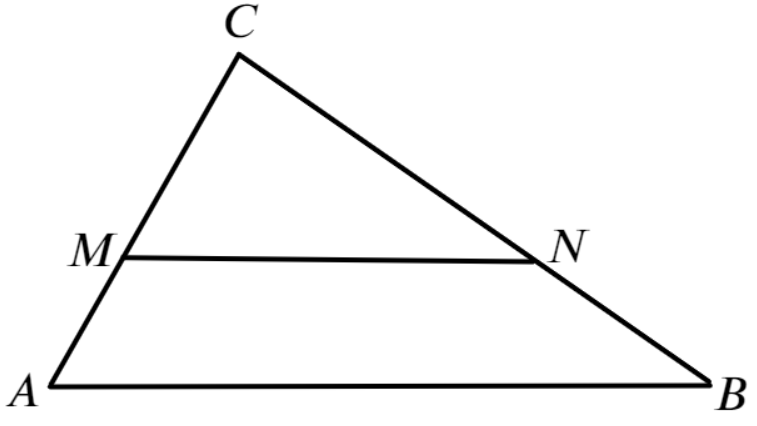
\includegraphics[scale=0.35]{g8-61.png}}
\end{figure}\\
Треугольники $MCN$ и $ABC$ подобны по двум углам (общий и соответственные при паралелльных прямых $MN$ и $AB$), коэффициент подобия равен $\cfrac{3}{3+2}=\cfrac{3}{5}.$ Тогда если $S_{\Delta ABC}=S,$ то $S_{\Delta MCN}=\cfrac{9}{25}S,$ а $S_{AMNB}=S-\cfrac{9}{25}S=\cfrac{16}{25}S,$ поэтому $\cfrac{S_{\Delta MCN}}{S_{AMNB}}=\cfrac{\cfrac{9}{25}S}{\cfrac{16}{25}S}=\cfrac{9}{16}.$\\
62. \begin{figure}[ht!]
\center{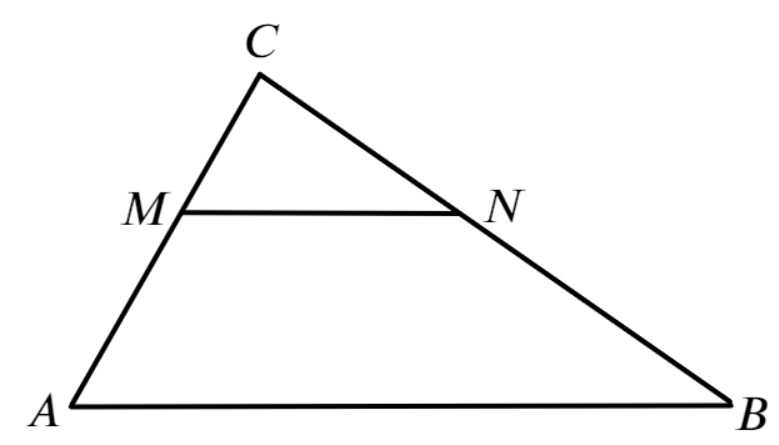
\includegraphics[scale=0.35]{g8-62.png}}
\end{figure}\\
Треугольники $MCN$ и $ABC$ подобны по двум углам (общий и соответственные при паралелльных прямых $MN$ и $AB$), коэффициент подобия равен $\cfrac{2}{3+2}=\cfrac{2}{5}.$ Тогда если $S_{\Delta ABC}=S,$ то $S_{\Delta MCN}=\cfrac{4}{25}S,$ а $S_{AMNB}=S-\cfrac{4}{25}S=\cfrac{21}{25}S,$ поэтому $\cfrac{S_{\Delta MCN}}{S_{AMNB}}=\cfrac{\cfrac{4}{25}S}{\cfrac{21}{25}S}=\cfrac{4}{21}.$\\
63. Пусть стороны равны $a$ и $b,$ тогда $\begin{cases}(a+b)\cdot2=34,\\ a^2+b^2=13^2.\end{cases}\Leftrightarrow
\begin{cases}b=17-a,\\ a^2+(17-a)^2=169.\end{cases}\Leftrightarrow$\\$
\begin{cases}b=17-a,\\ 2a^2-34a+120=0.\end{cases}\Leftrightarrow
\left[\begin{array}{l}\begin{cases}a=5\text{ см},\\ b=12\text{ см}.\end{cases}\\ \begin{cases}a=12\text{ см},\\ b=5\text{ см}.\end{cases}\end{array}
ight.$\\
64. \begin{figure}[ht!]
\center{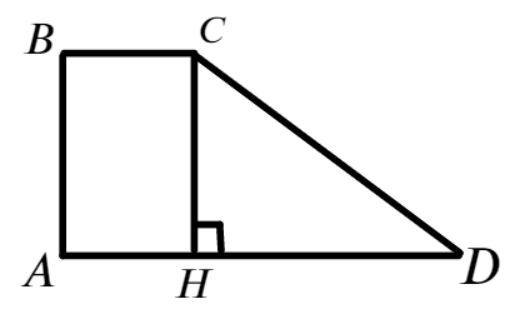
\includegraphics[scale=0.35]{g8-64.png}}
\end{figure}\\
Опустим высоту $CH,$ тогда $HD=6-2=4$см. По теореме Пифагора $CD=\sqrt{4^2+3^2}=5$см, тогда $\cos(D)=\cfrac{4}{5}.$\\
65. \begin{figure}[ht!]
\center{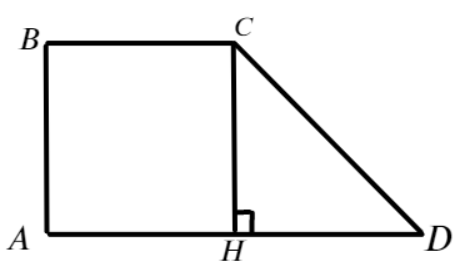
\includegraphics[scale=0.35]{g8-65.png}}
\end{figure}\\
Опустим высоту $CH,$ тогда $HD=8-5=3$см. По теореме Пифагора $CD=\sqrt{4^2+3^2}=5$см, тогда $\cos(D)=\cfrac{3}{5}.$\\
66. \begin{figure}[ht!]
\center{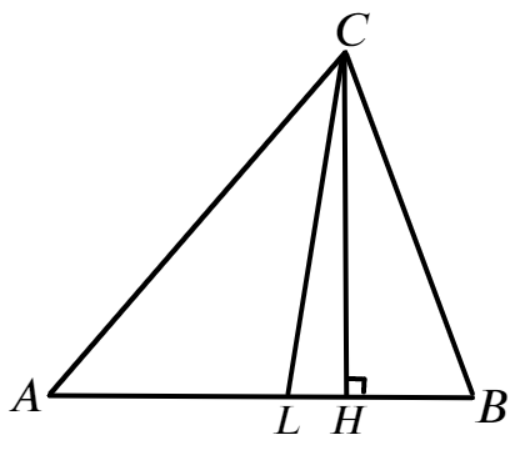
\includegraphics[scale=0.35]{g8-66.png}}
\end{figure}\\
Проведём высоту $CH$ и биссектрису $CL.$ Найдём $\angle C=180^\circ-48^\circ-76^\circ=56^\circ.$ Тогда $\angle BCL=56^\circ:2=28^\circ,\ \angle BCH=90^\circ-76^\circ=14^\circ,\ \angle LCH=28^\circ-14^\circ=14^\circ.$\\
67. \begin{figure}[ht!]
\center{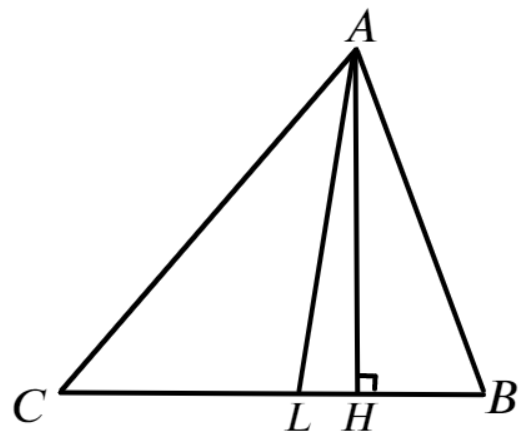
\includegraphics[scale=0.35]{g8-67.png}}
\end{figure}\\
Проведём высоту $AH$ и биссектрису $AL.$ Найдём $\angle A=180^\circ-64^\circ-24^\circ=92^\circ.$ Тогда $\angle BAL=92^\circ:2=46^\circ,\ \angle BAH=90^\circ-64^\circ=26^\circ,\ \angle LCH=46^\circ-26^\circ=20^\circ.$
ewpage
oindent
68. \begin{figure}[ht!]
\center{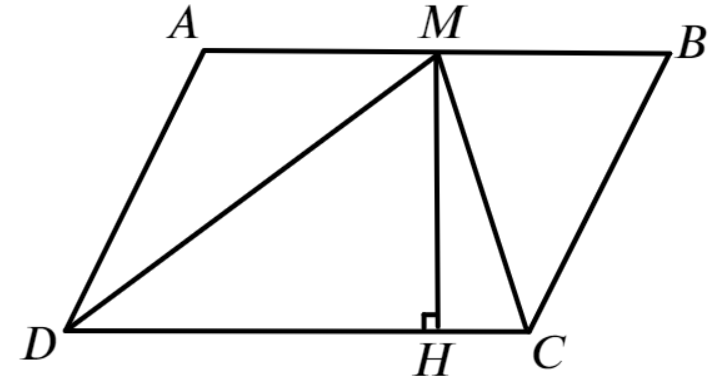
\includegraphics[scale=0.35]{g8-68.png}}
\end{figure}\\
Проведём перпендикуляр $MH,$ он является высотой треугольника и равен высоте параллелограмма. Так как $S_{\Delta MCD}=\cfrac{1}{2}MH\cdot CD,$ а $S_{ABCD}=MH\cdot CD,$ площадь параллелограмма в 2 раза больше и равна $2\cdot38=76\text{ см}^2.$\\
69. \begin{figure}[ht!]
\center{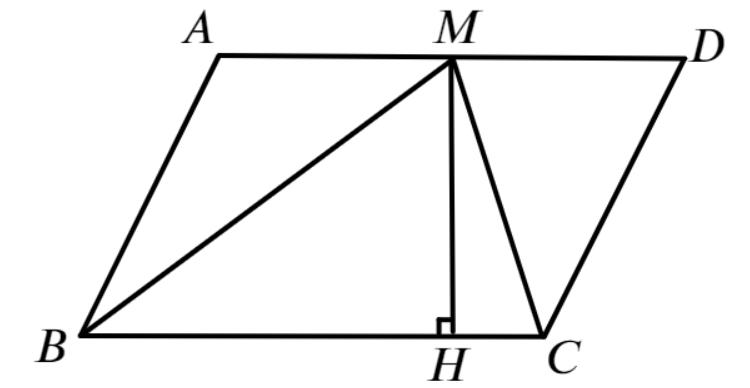
\includegraphics[scale=0.35]{g8-69.png}}
\end{figure}\\
Проведём перпендикуляр $MH,$ он является высотой треугольника и равен высоте параллелограмма. Так как $S_{\Delta MCB}=\cfrac{1}{2}MH\cdot CB,$ а $S_{ABCD}=MH\cdot CB,$ площадь параллелограмма в 2 раза больше и равна $2\cdot42=84\text{ см}^2.$\\
70. \begin{figure}[ht!]
\center{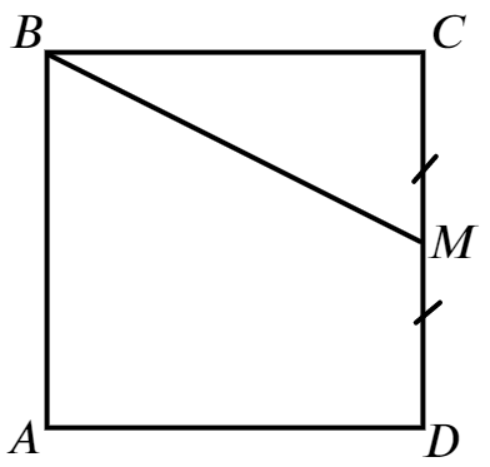
\includegraphics[scale=0.35]{g8-70.png}}
\end{figure}\\
Пусть сторона квадрата равна $a,$ тогда по теореме Пифагора для треугольника $BMC$ имеем $3^2=a^2+\cfrac{1}{4}a^2,\ a^2=\cfrac{36}{5}\text{ см}^2,$ а $S=a^2=\cfrac{36}{5}\text{ см}^2.$
ewpage
oindent
71. \begin{figure}[ht!]
\center{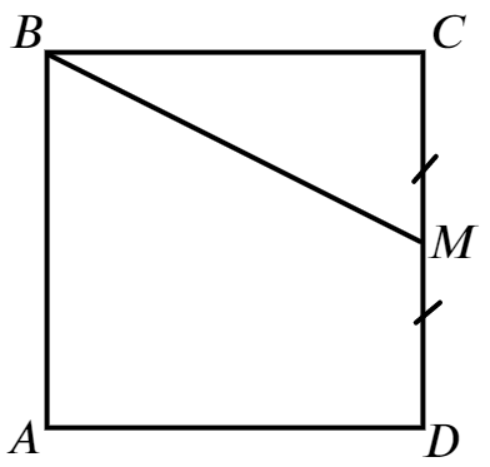
\includegraphics[scale=0.35]{g8-70.png}}
\end{figure}\\
Пусть сторона квадрата равна $a,$ тогда по теореме Пифагора для треугольника $BMC$ имеем $4^2=a^2+\cfrac{1}{4}a^2,\ a^2=\cfrac{64}{5}\text{ см}^2,$ а $S=a^2=\cfrac{64}{5}\text{ см}^2.$\\
72. \begin{figure}[ht!]
\center{\includegraphics[scale=0.35]{g8-71.png}}
\end{figure}\\
Проведём радиусы к точкам касания. Так как отрезки касательных, проведённых из одной точки, равны, имеем $AK=AM,\ BK=BL,\ CL=CM.$ Так как $AKOM$ прямоугольник и $AK=AM,$ он является квадратом и радиус окружности тоже равен $AK.$ Пусть $AK=AM=x,$ тогда $AB=x+3,\ AC=x+2,\ BC=3+2=5$ и по теореме Пифагора для треугольника $ABC$ получаем $(x+3)^2+(x+2)^2=5^2,\ x^2+6x+9+x^2+4x+4=25,\ 2x^2+10x-12=0,\ x=1\text{ см}.$\\
73. \begin{figure}[ht!]
\center{\includegraphics[scale=0.35]{g8-71.png}}
\end{figure}\\
Проведём радиусы к точкам касания. Так как отрезки касательных, проведённых из одной точки, равны, имеем $AK=AM,\ BK=BL,\ CL=CM.$ Так как $AKOM$ прямоугольник и $AK=AM,$ он является квадратом и радиус окружности тоже равен $AK.$ Пусть $AK=AM=x,$ тогда $AB=x+6,\ AC=x+4,\ BC=6+4=10$ и по теореме Пифагора для треугольника $ABC$ получаем $(x+6)^2+(x+4)^2=10^2,\ x^2+12x+36+x^2+8x+16=100,\ 2x^2+20x-48=0,\ x=2\text{ см}.$\\
74. \begin{figure}[ht!]
\center{\includegraphics[scale=0.35]{g8-74.png}}
\end{figure}\\
Проведём высоту $CH.$ Тогда $ABCH$ является прямоугольником, а так как $AB=BC,$ то и квадратом. Так как $\angle D=45^\circ,\ \angle HCD=90^\circ-45^\circ=45^\circ$ и треугольник $CHD$ является равнобедренным, $HD=CH=BC=AB.$ Пусть $BC=x,$ тогда $S_{ABCD}=\cfrac{1}{2}\cdot{x}\cdot(x+x+x)=\cfrac{3}{2}x^2=54,\ x^2=36,\ x=6$см.
ewpage
oindent
75. \begin{figure}[ht!]
\center{\includegraphics[scale=0.35]{g8-74.png}}
\end{figure}\\
Проведём высоту $CH.$ Тогда $ABCH$ является прямоугольником, а так как $AB=BC,$ то и квадратом. Так как $\angle D=45^\circ,\ \angle HCD=90^\circ-45^\circ=45^\circ$ и треугольник $CHD$ является равнобедренным, $HD=CH=BC=AB.$ Пусть $BC=x,$ тогда $S_{ABCD}=\cfrac{1}{2}\cdot{x}\cdot(x+x+x)=\cfrac{3}{2}x^2=24,\ x^2=16,\ x=4$см.\\
76. \begin{figure}[ht!]
\center{\includegraphics[scale=0.35]{g8-76.png}}
\end{figure}\\
В ромбе диагонали перпендикулярны и делятся (как и в любом параллелограмме) точкой пересечения пополам. Пусть $BD=12,$ тогда $BO=12:2=6$ и по теореме Пифагора $AO=\sqrt{AB^2-BO^2}=\sqrt{100-36}=8,$ значит $AC=2AO=16.$\\
77. \begin{figure}[ht!]
\center{\includegraphics[scale=0.35]{g8-76.png}}
\end{figure}\\
В ромбе диагонали перпендикулярны и делятся (как и в любом параллелограмме) точкой пересечения пополам. Пусть $AC=18,$ тогда $AO=16:2=8$ и по теореме Пифагора $BO=\sqrt{AB^2-AO^2}=\sqrt{100-64}=6,$ значит $BD=2BO=12.$\\
78. \begin{figure}[ht!]
\center{\includegraphics[scale=0.35]{g8-78.png}}
\end{figure}\\
Из четырёхугольника $OC_1BA_1:\ \angle C_1OA_1=360^\circ-90^\circ-90^\circ-70^\circ=110^\circ.$ Так как углом между прямыми по определению считается острый (или прямой) угол, ответом будет $180^\circ-110^\circ=70^\circ.$
ewpage
oindent
79. \begin{figure}[ht!]
\center{\includegraphics[scale=0.35]{g8-78.png}}
\end{figure}\\
Из четырёхугольника $OC_1BA_1:\ \angle C_1OA_1=360^\circ-90^\circ-90^\circ-50^\circ=130^\circ.$ Так как углом между прямыми по определению считается острый (или прямой) угол, ответом будет $180^\circ-130^\circ=50^\circ.$\\
80. \begin{figure}[ht!]
\center{\includegraphics[scale=0.35]{g8-80.png}}
\end{figure}\\
Треугольники $AMN$ и $CND$ подобны по двум углам ($MNA$ и $CND$ вертикальные, $MAN$ и $NCD$ накрест лежащие), поэтому $\cfrac{NC}{NA}=\cfrac{CD}{AM}=\cfrac{AB}{AM}=2,$ значит $NC=2NA$ и $NC+NA=18,$ откуда $NA=6,\ NC=12.$\\
81. \begin{figure}[ht!]
\center{\includegraphics[scale=0.35]{g8-80.png}}
\end{figure}\\
Треугольники $AMN$ и $CND$ подобны по двум углам ($MNA$ и $CND$ вертикальные, $MAN$ и $NCD$ накрест лежащие), поэтому $\cfrac{NC}{NA}=\cfrac{CD}{AM}=\cfrac{AB}{AM}=2,$ значит $NC=2NA$ и $NC+NA=15,$ откуда $NA=5,\ NC=10.$\\
82. По определению $tg(\alpha)=\cfrac{BC}{AC},$ значит $BC=AC\ tg(\alpha)=m\ tg(\alpha).$\\
83. По определению $ctg(\alpha)=\cfrac{BC}{AC},$ значит $BC=AC\ ctg(\alpha)=m\ ctg(\alpha).$\\
84. $S=\cfrac{1}{2}d_1d_2=\cfrac{1}{2}\cdot14\cdot13=91\text{ см}^2.$\\
85. $S=\cfrac{1}{2}d_1d_2=\cfrac{1}{2}\cdot16\cdot11=88\text{ см}^2.$\\
86. У окружности, описанной около прямоугольного треугольника, центр находится в середине его гипотенузы, а радиус равен её половине. Так как напротив угла в $30^\circ$ лежит катет, равный половине гипотенузы, $AB=2AC=36$см, тогда радиус $R=36:2=18$см.\\
87. У окружности, описанной около прямоугольного треугольника, центр находится в середине его гипотенузы, а радиус равен её половине. Так как напротив угла в $30^\circ$ лежит катет, равный половине гипотенузы, $AB=2BC=24$см, тогда радиус $R=24:2=12$см.\\
88. Раз $\sin \angle A=\cfrac{2}{3},$ так как угол $A$ является острым, $\cos \angle A=\sqrt{1-\sin^2 \angle A}=\sqrt{1-\cfrac{4}{9}}=\cfrac{\sqrt{5}}{3}.$ Тогда $tg\ \angle A=\cfrac{\sin \angle A}{\cos \angle A}=\cfrac{\cfrac{2}{3}}{\cfrac{\sqrt{5}}{3}}=\cfrac{2\sqrt{5}}{5}.$\\
89. Раз $\cos \angle A=\cfrac{2}{3},$ так как угол $A$ является острым, $\sin \angle A=\sqrt{1-\cos^2 \angle A}=\sqrt{1-\cfrac{4}{9}}=\cfrac{\sqrt{5}}{3}.$ Тогда $tg\ \angle A=\cfrac{\sin \angle A}{\cos \angle A}=\cfrac{\cfrac{\sqrt{5}}{3}}{\cfrac{2}{3}}=\cfrac{\sqrt{5}}{2}.$\\
90. \begin{figure}[ht!]
\center{\includegraphics[scale=0.35]{g8-90.png}}
\end{figure}\\
Возможны два случая: треугольник может быть остроугольным или тупоугольным. В обоих случаях необходимо рассмотреть четырёхугольник $C_1BA_1O:$ в первом случае $\angle B =360^\circ-90^\circ-90^\circ-140^\circ=40^\circ,$ а во втором --- $\angle B=\angle C_1BA_1=360^\circ-90^\circ-90^\circ-40^\circ=140^\circ.$ В первом случае мы воспользовались тем, что по определению углом между прямыми называется острый (или прямой) угол.\\
91. \begin{figure}[ht!]
\center{\includegraphics[scale=0.35]{g8-90.png}}
\end{figure}\\
Возможны два случая: треугольник может быть остроугольным или тупоугольным. В обоих случаях необходимо рассмотреть четырёхугольник $C_1BA_1O:$ в первом случае $\angle B =360^\circ-90^\circ-90^\circ-100^\circ=80^\circ,$ а во втором --- $\angle B=\angle C_1BA_1=360^\circ-90^\circ-90^\circ-80^\circ=100^\circ.$ В первом случае мы воспользовались тем, что по определению углом между прямыми называется острый (или прямой) угол.\\
92. \begin{figure}[ht!]
\center{\includegraphics[scale=0.35]{g8-92.png}}
\end{figure}\\
Проведём диагональ $AC,$ тогда $MN$ является средней линией в треугольнике $ABC$ и треугольник $ABC$ подобен треугольнику $MBN$ с коэффициентом 2 (по двум сторонам и общему углу между ними), значит $S_{\Delta MBN}=\cfrac{1}{4}S_{\Delta ABC}.$ Аналогично $S_{\Delta DPQ}=\cfrac{1}{4}S_{\Delta ACD},\  S_{\Delta CNP}=\cfrac{1}{4}S_{\Delta BCD},\ S_{\Delta AMQ}=\cfrac{1}{4}S_{\Delta ABD},$ тогда $S_{MNPQ}=S-S_{\Delta MBN}-S_{\Delta DPQ}-S_{\Delta CNP}-S_{\Delta AMQ}=
S-\cfrac{1}{4}S_{\Delta ABC}-\cfrac{1}{4}S_{\Delta ACD}-\cfrac{1}{4}S_{\Delta BCD}-\cfrac{1}{4}S_{\Delta ABD}=S-\cfrac{1}{4}(S_{\Delta ABC}+S_{\Delta ACD}+
S_{\Delta BCD}+S_{\Delta ABD})=S-\cfrac{1}{4}\cdot2S=\cfrac{S}{2}.$\\
93. \begin{figure}[ht!]
\center{\includegraphics[scale=0.35]{g8-92.png}}
\end{figure}\\
Проведём диагональ $AC,$ тогда $MN$ является средней линией в треугольнике $ABC$ и треугольник $ABC$ подобен треугольнику $MBN$ с коэффициентом 2 (по двум сторонам и общему углу между ними), значит $S_{\Delta MBN}=\cfrac{1}{4}S_{\Delta ABC}.$ Аналогично $S_{\Delta DPQ}=\cfrac{1}{4}S_{\Delta ACD},\  S_{\Delta CNP}=\cfrac{1}{4}S_{\Delta BCD},\ S_{\Delta AMQ}=\cfrac{1}{4}S_{\Delta ABD}.$ Пусть $S_{ABCD}=S_1,$ тогда $S_{MNPQ}=S_1-S_{\Delta MBN}-S_{\Delta DPQ}-S_{\Delta CNP}-S_{\Delta AMQ}=
S_1-\cfrac{1}{4}S_{\Delta ABC}-\cfrac{1}{4}S_{\Delta ACD}-\cfrac{1}{4}S_{\Delta BCD}-\cfrac{1}{4}S_{\Delta ABD}=S_1-\cfrac{1}{4}(S_{\Delta ABC}+S_{\Delta ACD}+
S_{\Delta BCD}+S_{\Delta ABD})=S_1-\cfrac{1}{4}\cdot2S_1=\cfrac{S_1}{2},$ значит $S_1=2S.$\\
94. По теореме Пифагора $AB=\sqrt{3^2+4^2}=5.$ В прямоугольном треугольнике медиана, проведённая из прямого угла, равна половине гипотенузы, значит $CK=\cfrac{5}{2}.$\\
95. \begin{figure}[ht!]
\center{\includegraphics[scale=0.35]{g8-95.png}}
\end{figure}\\
Точки касания окружностей лежат на одной прямой с их центрами, поэтому $O_1O_2=2+4=6,\ O_1O_3=2+6=8,\ O_2O_3=4+6=10.$ Так как $6^2+8^2=10^2,$ по обратной теореме Пифагора треугольник $O_1O_2O_3$ является прямоугольным. Посчитаем его площадь двумя способами. С одной стороны, она равна $6\cdot8:2=24,$ а с другой $rp=r\cdot\cfrac{6+8+10}{2}=12r.$ Значит, $r=24:12=2.$
ewpage
oindent
96. \begin{figure}[ht!]
\center{\includegraphics[scale=0.35]{g8-96.png}}
\end{figure}\\
В ромбе диагонали перпендикулярны и являются биссектрисами его углов, поэтому треугольник $ABO$ является прямоугольным и $\angle BAO=120^\circ:2=60^\circ.$ Тогда $AO=AB\cos(60^\circ)=20\cdot\cfrac{1}{2}=10.$\\
97. Из определения тригонометрических функций имеем $BC=c\sin(\alpha),\ AC=c\cos(\alpha),$ тогда $P=c+c\sin(\alpha)+c\cos(\alpha)=c(1+\sin(\alpha)+\cos(\alpha)).$\\
98. Из определения тригонометрических функций имеем $BC=c\sin(\alpha),\ AC=c\cos(\alpha),$ тогда $S=\cfrac{c\sin(\alpha)\cdot c\cos(\alpha)}{2}=\cfrac{c^2\sin(\alpha)\cos(\alpha)}{2}.$\\
99. \begin{figure}[ht!]
\center{\includegraphics[scale=0.35]{g8-99.png}}
\end{figure}\\
Продлим боковые стороны трапеции до точки их пересечения $E.$ Тогда $\angle E=180^\circ-53^\circ-37^\circ=90^\circ.$ Пусть $N$ --- середина $AD,$ тогда $EN$ является медианой прямоугольного треугольника, проведённой из прямого угла, поэтому $EN=\cfrac{1}{2}AD=\cfrac{1}{2}\cdot18=9$см.\\
100. \begin{figure}[ht!]
\center{\includegraphics[scale=0.35]{g8-99.png}}
\end{figure}\\
Продлим боковые стороны трапеции до точки их пересечения $E.$ Тогда $\angle E=180^\circ-58^\circ-32^\circ=90^\circ.$ Пусть $N$ --- середина $AD,$ тогда $EN$ является медианой прямоугольного треугольника, проведённой из прямого угла, поэтому $EN=\cfrac{1}{2}AD=\cfrac{1}{2}\cdot22=11$см.
ewpage
oindent
101. \begin{figure}[ht!]
\center{\includegraphics[scale=0.35]{g8-102.png}}
\end{figure}\\
Соединим центры окружностей друг с другом и с точками касания. Так как центры окружностей лежат на одной прямой с точкой касания, а радиусы перпендикулярны касательной, $AO_1O_2B$ --- прямоугольная трапеция, в которой $AO_1=4R,\ BO_2=R,\ O_1O_2=4R+R=5R,\ AB=8$см. Опустим высоту $O_2H,$ тогда $O_1H=4R-R=3R,$ а $O_2H=AB=8$см. По теореме Пифагора для треугольника $O_1HO_2$ имеем $25R^2=9R^2+64,\ R^2=4,\ R=2$см. Значит, радиусы окружностей равны 2 см и $2\cdot4=8$см.\\
102. \begin{figure}[ht!]
\center{\includegraphics[scale=0.35]{g8-102.png}}
\end{figure}\\
Соединим центры окружностей друг с другом и с точками касания. Так как центры окружностей лежат на одной прямой с точкой касания, а радиусы перпендикулярны касательной, $AO_1O_2B$ --- прямоугольная трапеция, в которой $AO_1=4R,\ BO_2=R,\ O_1O_2=4R+R=5R,\ AB=16$см. Опустим высоту $O_2H,$ тогда $O_1H=4R-R=3R,$ а $O_2H=AB=16$см. По теореме Пифагора для треугольника $O_1HO_2$ имеем $25R^2=9R^2+256,\ R^2=16,\ R=4$см. Значит, радиусы окружностей равны 4 см и $4\cdot4=16$см.\\
103. \begin{figure}[ht!]
\center{\includegraphics[scale=0.35]{g8-103.png}}
\end{figure}\\
Найдём $\angle C=\angle A=(180^\circ-120^\circ):2=30^\circ.$ Тогда в прямоугольном треугольнике $AHC$ катет $AH$ лежит напротив угла в $30^\circ$ и $AC=2AH=2\cdot15=30$см.
ewpage
oindent
104. \begin{figure}[ht!]
\center{\includegraphics[scale=0.35]{g8-103.png}}
\end{figure}\\
Найдём $\angle C=\angle A=(180^\circ-120^\circ):2=30^\circ.$ Тогда в прямоугольном треугольнике $AHC$ катет $AH$ лежит напротив угла в $30^\circ$ и
$AH=\cfrac{1}{2}AC=\cfrac{1}{2}\cdot30=15$см.\\
105. \begin{figure}[ht!]
\center{\includegraphics[scale=0.35]{g8-105.png}}
\end{figure}\\
Треугольники $AOD$ и $BOC$ подобны по двум углам ($\angle AOD$ и $\angle BOC$ вертикальные, $\angle BCO$ и $\angle OAD$ накрест лежащие). Раз
$\cfrac{S_{\Delta AOD}}{S_{\Delta BOC}}=16,$ коэффициент подобия равен $\sqrt{16}=4,$ поэтому $\cfrac{BC}{AD}=\cfrac{1}{4}.$\\
106. \begin{figure}[ht!]
\center{\includegraphics[scale=0.35]{g8-105.png}}
\end{figure}\\
Треугольники $AOD$ и $BOC$ подобны по двум углам ($\angle AOD$ и $\angle BOC$ вертикальные, $\angle BCO$ и $\angle OAD$ накрест лежащие). Раз
$\cfrac{S_{\Delta AOD}}{S_{\Delta BOC}}=25,$ коэффициент подобия равен $\sqrt{25}=5,$ поэтому $\cfrac{BC}{AD}=\cfrac{1}{5}.$\\
107. Так как $(\sqrt{2})^2+(\sqrt{7})^2=3^2,$ по обратной теореме Пифагора этот треугольник является прямоугольным, а значит $S=\cfrac{\sqrt{2}\cdot\sqrt{7}}{2}=\cfrac{\sqrt{14}}{2}.$\\
108. Так как $(\sqrt{5})^2+(\sqrt{11})^2=4^2,$ по обратной теореме Пифагора этот треугольник является прямоугольным, а значит $S=\cfrac{\sqrt{5}\cdot\sqrt{11}}{2}=\cfrac{\sqrt{55}}{2}.$
ewpage
oindent
109. \begin{figure}[ht!]
\center{\includegraphics[scale=0.35]{g8-109.png}}
\end{figure}\\
Найдём $\angle A=180^\circ-120^\circ=60^\circ.$ Опустим перпендикуляры $KL$ и $BH,$ тогда $\angle ABH=90^\circ-60^\circ=30^\circ,$ поэтому $AH=\cfrac{1}{2}AB=\cfrac{1}{2}\cdot4=2,\ BH=KL=\sqrt{4^2-2^2}=2\sqrt{3}.$ В треугольнике $AKL:\ AL=AH+HL=2+2=4,$ тогда $AK=\sqrt{4^2+(2\sqrt{3})^2}=2\sqrt{7}$ по теореме Пифагора.\\
110. \begin{figure}[ht!]
\center{\includegraphics[scale=0.35]{g8-109.png}}
\end{figure}\\
Найдём $\angle A=180^\circ-120^\circ=60^\circ.$ Опустим перпендикуляры $KL$ и $BH,$ тогда $\angle ABH=90^\circ-60^\circ=30^\circ,$ поэтому $AH=\cfrac{1}{2}AB=\cfrac{1}{2}\cdot6=3,\ BH=KL=\sqrt{6^2-3^2}=3\sqrt{3}.$ В треугольнике $AKL:\ AL=AH+HL=3+3=6,$ тогда $AK=\sqrt{6^2+(3\sqrt{3})^2}=3\sqrt{7}$ по теореме Пифагора.\\
111. \begin{figure}[ht!]
\center{\includegraphics[scale=0.35]{g8-111.png}}
\end{figure}\\
Найдём $\angle A=90^\circ-60^\circ=30^\circ,$ тогда $\angle C=90^\circ-30^\circ=60^\circ,\ \angle CBH=90^\circ-60^\circ=30^\circ.$ По теореме о прямоугольном треугольнике с углом в $30^\circ$ для треугольников $CBH$ и $ABC$ имеем соотношения $BC=2CH=16,\ AC=2BC=32.$ Тогда $AH=AC-CH=32-8=24.$\\
112. \begin{figure}[ht!]
\center{\includegraphics[scale=0.35]{g8-111.png}}
\end{figure}\\
Найдём $\angle A=90^\circ-60^\circ=30^\circ,\ \angle CBH=90^\circ-60^\circ=30^\circ.$ Пусть $CH=x,$ тогда по теореме о прямоугольном треугольнике с углом в $30^\circ$ для треугольников $CBH$ и $ABC$ имеем соотношения $BC=2x,\ AC=2BC=4x.$ Тогда $AC=AH+HC,\ 4x=12+x,\ x=4.$
ewpage
oindent
113. \begin{figure}[ht!]
\center{\includegraphics[scale=0.35]{g8-111.png}}
\end{figure}\\
Найдём $\angle A=90^\circ-60^\circ=30^\circ,$ тогда $\angle C=90^\circ-30^\circ=60^\circ,\ \angle CBH=90^\circ-60^\circ=30^\circ.$ По теореме о прямоугольном треугольнике с углом в $30^\circ$ для треугольников $CBH$ и $ABC$ имеем соотношения $BC=2CH=8,\ AC=2BC=16.$ Тогда $AH=AC-CH=16-4=12.$\\
114. \begin{figure}[ht!]
\center{\includegraphics[scale=0.35]{g8-111.png}}
\end{figure}\\
Найдём $\angle A=90^\circ-60^\circ=30^\circ,\ \angle CBH=90^\circ-60^\circ=30^\circ.$ Пусть $CH=x,$ тогда по теореме о прямоугольном треугольнике с углом в $30^\circ$ для треугольников $CBH$ и $ABC$ имеем соотношения $BC=2x,\ AC=2BC=4x.$ Тогда $AC=AH+HC,\ 4x=18+x,\ x=6.$\\
115. \begin{figure}[ht!]
\center{\includegraphics[scale=0.35]{g8-115.png}}
\end{figure}\\
Треугольники $AOB,\ BOC,\ COD$ и $AOD$ являются прямоугольными. Пусть $AO=x,\ CO=4-x,\ BO=y,\ DO=5-y.$ Тогда $S_{ABCD}=S_{\Delta AOB}+S_{\Delta BOC}+S_{\Delta COD}+S_{\Delta AOD}=\cfrac{xy}{2}+\cfrac{y(4-x)}{2}+\cfrac{(4-x)(5-y)}{2}+\cfrac{x(5-y)}{2}=\cfrac{xy+4y-xy+20-4y-5x+xy+5x-xy}{2}=10.$\\
116. \begin{figure}[ht!]
\center{\includegraphics[scale=0.35]{g8-115.png}}
\end{figure}\\
Треугольники $AOB,\ BOC,\ COD$ и $AOD$ являются прямоугольными. Пусть $AO=x,\ CO=5-x,\ BO=y,\ DO=8-y.$ Тогда $S_{ABCD}=S_{\Delta AOB}+S_{\Delta BOC}+S_{\Delta COD}+S_{\Delta AOD}=\cfrac{xy}{2}+\cfrac{y(5-x)}{2}+\cfrac{(5-x)(8-y)}{2}+\cfrac{x(8-y)}{2}=\cfrac{xy+5y-xy+40-5y-8x+xy+8x-xy}{2}=20.$
ewpage
oindent
117. \begin{figure}[ht!]
\center{\includegraphics[scale=0.35]{g8-115.png}}
\end{figure}\\
Треугольники $AOB,\ BOC,\ COD$ и $AOD$ являются прямоугольными. Пусть $AO=x,\ CO=6-x,\ BO=y,\ DO=7-y.$ Тогда $S_{ABCD}=S_{\Delta AOB}+S_{\Delta BOC}+S_{\Delta COD}+S_{\Delta AOD}=\cfrac{xy}{2}+\cfrac{y(6-x)}{2}+\cfrac{(6-x)(7-y)}{2}+\cfrac{x(7-y)}{2}=\cfrac{xy+6y-xy+42-6y-7x+xy+7x-xy}{2}=21.$\\
118. \begin{figure}[ht!]
\center{\includegraphics[scale=0.35]{g8-115.png}}
\end{figure}\\
Треугольники $AOB,\ BOC,\ COD$ и $AOD$ являются прямоугольными. Пусть $AO=x,\ CO=5-x,\ BO=y,\ DO=6-y.$ Тогда $S_{ABCD}=S_{\Delta AOB}+S_{\Delta BOC}+S_{\Delta COD}+S_{\Delta AOD}=\cfrac{xy}{2}+\cfrac{y(5-x)}{2}+\cfrac{(5-x)(6-y)}{2}+\cfrac{x(6-y)}{2}=\cfrac{xy+5y-xy+30-5y-6x+xy+6x-xy}{2}=15.$\\
119. \begin{figure}[ht!]
\center{\includegraphics[scale=0.35]{g8-119.png}}
\end{figure}\\
Так как $KD=DL=KL,$ треугольник $KDL$ является правильным и все его углы равны по $60^\circ,$ тогда $\angle KDC=90^\circ-60^\circ=30^\circ$ и $CD=KD\cos(30^\circ)=6\cdot\cfrac{\sqrt{3}}{2}=3\sqrt{3}=AB,\ AL=AB\ tg(60^\circ)=3\sqrt{3}\cdot\sqrt{3}=9.$ Таким образом, $S_{ABCD}=AB\cdot AD=3\sqrt{3}\cdot(9+6)=45\sqrt{3}.$\\
120. \begin{figure}[ht!]
\center{\includegraphics[scale=0.35]{g8-121.png}}
\end{figure}\\
Так как $KD=DL=KL,$ треугольник $KDL$ является правильным и все его углы равны по $60^\circ,$ тогда $\angle KDC=90^\circ-60^\circ=30^\circ$ и $CD=KD\cos(30^\circ)=8\cdot\cfrac{\sqrt{3}}{2}=4\sqrt{3}=AB,\ AL=AB\ tg(45^\circ)=4\sqrt{3}\cdot1=4\sqrt{3}.$ Таким образом, $S_{ABCD}=AB\cdot AD=4\sqrt{3}\cdot(4\sqrt{3}+8)=48+32\sqrt{3}.$\\
121.\begin{figure}[ht!]
\center{\includegraphics[scale=0.35]{g8-119.png}}
\end{figure}\\
Так как $KD=DL=KL,$ треугольник $KDL$ является правильным и все его углы равны по $60^\circ,$ тогда $\angle KDC=90^\circ-60^\circ=30^\circ$ и $CD=KD\cos(30^\circ)=8\cdot\cfrac{\sqrt{3}}{2}=4\sqrt{3}=AB,\ AL=AB\ tg(60^\circ)=4\sqrt{3}\cdot\sqrt{3}=12.$ Таким образом, $S_{ABCD}=AB\cdot AD=4\sqrt{3}\cdot(12+8)=80\sqrt{3}.$\\
122. \begin{figure}[ht!]
\center{\includegraphics[scale=0.35]{g8-121.png}}
\end{figure}\\
Так как $KD=DL=KL,$ треугольник $KDL$ является правильным и все его углы равны по $60^\circ,$ тогда $\angle KDC=90^\circ-60^\circ=30^\circ$ и $CD=KD\cos(30^\circ)=6\cdot\cfrac{\sqrt{3}}{2}=3\sqrt{3}=AB,\ AL=AB\ tg(45^\circ)=3\sqrt{3}\cdot1=3\sqrt{3}.$ Таким образом, $S_{ABCD}=AB\cdot AD=3\sqrt{3}\cdot(3\sqrt{3}+6)=27+18\sqrt{3}.$\\
123. \begin{figure}[ht!]
\center{\includegraphics[scale=0.35]{g8-123.png}}
\end{figure}\\
Опустим перпендикуляры $MH_1,\ MH_2$ и $MH_3.$ Тогда по гипотенузе (общей) и углу равны следующие пары треугольников: $MCH_2$ с $MCH_3$ и $MCH_1$ с $MCH_3.$ Тогда $MH_1=MH_3=MH_2=4.$
ewpage
oindent
124. \begin{figure}[ht!]
\center{\includegraphics[scale=0.35]{g8-124.png}}
\end{figure}\\
В треугольниках $ABP$ и $DCP$ медиана совпадает с высотой, значит они равнобедренные и $AP=BP,\ DP=CP.$ Тогда треугольники $APD$ и $BPC$ равны по трём сторонам ($AP=BP,\ DP=CP,\ BC=AD,$ значит $\angle BCP=\angle ADP=30^\circ.$\\
125. \begin{figure}[ht!]
\center{\includegraphics[scale=0.35]{g8-125.png}}
\end{figure}\\
Отметим равные углы, на которые делят угол биссектрисы и накрест лежащие: $\angle MAK=\angle MAB=\angle AMK$ и $\angle NBM=\angle MBA=\angle BMN.$ Тогда треугольники $AKM$ и $BNM$ являются равнобедренными и $AK=KM,\ BN=NM.$ Запишем разность $P_{\Delta ABC}-P_{\Delta KCN}=AB+AK+KC+CN+BN-CK-KM-NM-CN=AB=12-8=4.$\\
126. \begin{figure}[ht!]
\center{\includegraphics[scale=0.35]{g8-126.png}}
\end{figure}\\
Отметим равные углы, на которые делят угол биссектрисы, вертикальные и накрест лежащие: $\angle MAK=\angle CAD=\angle DAF=\angle AMK$ и $\angle NBM=\angle CBE=\angle EBG=\angle BMN.$ Тогда треугольники $AKM$ и $BNM$ являются равнобедренными и $AK=KM,\ BN=NM.$ Запишем разность $P_{\Delta CKN}-P_{\Delta ABC}=AC+AK+CB+BN+KN-AC-CB-AB=KM+MN+KN-AB=2KN-AB=8-AB=22-18,\ AB=4.$ Но тогда в четырёхугольнике $AKNB$ противоположные стороны $AB$ и $KN$ равны и параллельны, а значит он является параллелограммом и $AK\parallel BN,$ что невозможно (продолжения стороны треугольника не могут быть параллельны). Значит, описанная в задаче ситуация невозможна.
ewpage
oindent
127. \begin{figure}[ht!]
\center{\includegraphics[scale=0.35]{g8-127.png}}
\end{figure}\\
По теореме об основании биссектрисы $\cfrac{BD}{DC}=\cfrac{AB}{AC}=\cfrac{3}{5}.$ У треугольников $ABD$ и $ACD$ общая высота, опущенная из точки $A,$ значит $\cfrac{S_{\Delta ABD}}{S_{\Delta ACD}}=\cfrac{BD}{DC}=\cfrac{3}{5},$ значит $S_{\Delta ACD}=S_{\Delta ABD}\cdot \cfrac{5}{3}=9\cdot\cfrac{5}{3}=15\text{ см}^2.$\\
128. \begin{figure}[ht!]
\center{\includegraphics[scale=0.35]{g8-128.png}}
\end{figure}\\
По теореме об основании биссектрисы $\cfrac{AM}{MC}=\cfrac{AB}{AC}.$ У треугольников $ABM$ и $BCM$ общая высота, опущенная из точки $B,$ значит $\cfrac{S_{\Delta ABM}}{S_{\Delta BCM}}=\cfrac{1}{3}=\cfrac{AM}{MC}=\cfrac{AB}{AC},$ значит $AB=AC\cdot \cfrac{1}{3}=12\cdot\cfrac{1}{3}=4\text{ см}.$\\
129. \begin{figure}[ht!]
\center{\includegraphics[scale=0.35]{g8-129.png}}
\end{figure}\\
Опусти высоту $KH$ из точки $K,$ она равна также и высоте параллелограмма. Тогда $S_{\Delta CDK}=\cfrac{1}{2}\cdot KH\cdot CD,\ S_{ABCD}=KH\cdot CD\Rightarrow
S_{ABCD}=2S_{\Delta CDK}=56.$\\
130. \begin{figure}[ht!]
\center{\includegraphics[scale=0.35]{g8-129.png}}
\end{figure}\\
Опусти высоту $LH$ из точки $L,$ она равна также и высоте параллелограмма. Тогда $S_{\Delta ALD}=\cfrac{1}{2}\cdot LH\cdot AD,\ S_{ABCD}=LH\cdot AD\Rightarrow
S_{ABCD}=2S_{\Delta ALD}=46.$
ewpage
oindent
131. \begin{figure}[ht!]
\center{\includegraphics[scale=0.35]{g8-131.png}}
\end{figure}\\
В четырёхугольнике $AB_1A_1B$ угол, образованный стороной $AB_1$ и диагональю $BB_1,$ равен углу, образованному стороной $BA_1$ и диагональю $AA_1,$ значит он является вписанным. Тогда $\angle B_1A_1B+\angle BAC=180^\circ,\ \angle B_1A_1B=180^\circ-32^\circ=148^\circ.$ Угол $\angle CA_1B_1$ является смежным к нему, значит $\angle CA_1B_1=180^\circ-148^\circ=32^\circ.$\\
132. \begin{figure}[ht!]
\center{\includegraphics[scale=0.35]{g8-131.png}}
\end{figure}\\
В четырёхугольнике $AB_1A_1B$ угол, образованный стороной $AB_1$ и диагональю $BB_1,$ равен углу, образованному стороной $BA_1$ и диагональю $AA_1,$ значит он является вписанным. Тогда $\angle A_1B_1A+\angle CBA=180^\circ,\ \angle A_1B_1A=180^\circ-17^\circ=163^\circ.$ Угол $\angle CB_1A_1$ является смежным к нему, значит $\angle CB_1A_1=180^\circ-163^\circ=17^\circ.$\\
133. \begin{figure}[ht!]
\center{\includegraphics[scale=0.35]{g8-133.png}}
\end{figure}\\
Продлим боковые стороны трапеции до пересечения, тогда точка их пересечения лежит на одной прямой с серединами оснований (и с точкой пересечения диагоналей, но в нашей задаче это не требуется). Тогда $\angle AED=180^\circ-12^\circ-78^\circ=90^\circ.$ Отрезки $EN$ и $EM$ являются медианами, проведёнными из прямого угла, значит $MN=EN-EM=\cfrac{1}{2}AD-\cfrac{1}{2}BC=\cfrac{1}{2}(AD-BC)=\cfrac{1}{2}\cdot5=2,5$см.
ewpage
oindent
134. \begin{figure}[ht!]
\center{\includegraphics[scale=0.35]{g8-133.png}}
\end{figure}\\
Продлим боковые стороны трапеции до пересечения, тогда точка их пересечения лежит на одной прямой с серединами оснований (и с точкой пересечения диагоналей, но в нашей задаче это не требуется). Тогда $\angle AED=180^\circ-12^\circ-78^\circ=90^\circ.$ Отрезки $EN$ и $EM$ являются медианами, проведёнными из прямого угла, значит $MN=EN-EM=\cfrac{1}{2}AD-\cfrac{1}{2}BC=\cfrac{1}{2}(AD-BC)=\cfrac{1}{2}\cdot3=1,5$см.\\
135. \begin{figure}[ht!]
\center{\includegraphics[scale=0.35]{g8-135.png}}
\end{figure}\\
Проведём медиану $BM$ и высоту $BH$ из прямого угла. Тогда $BM=\cfrac{1}{2}AC=\cfrac{1}{2}\cdot12=6$ и в прямоугольном треугольнике $BMH$ катет $BH$ в 2 раза меньше гипотенузы $BM,$ а значит $\angle BMH=30^\circ, \angle BMA=180^\circ-30^\circ=150^\circ.$ Треугольник $ABM$ является равнобедренным (так как медиана, проведённая из прямого угла, равна половине гипотенузы), значит $\angle B=(180^\circ-150^\circ):2=15^\circ,$ а тогда $\angle C=90^\circ-15^\circ=75^\circ.$\\
136. \begin{figure}[ht!]
\center{\includegraphics[scale=0.35]{g8-135.png}}
\end{figure}\\
Проведём медиану $BM$ и высоту $BH$ из прямого угла. Тогда $BM=\cfrac{1}{2}AC=\cfrac{1}{2}\cdot16=8$ и в прямоугольном треугольнике $BMH$ катет $BH$ в 2 раза меньше гипотенузы $BM,$ а значит $\angle BMH=30^\circ, \angle BMA=180^\circ-30^\circ=150^\circ.$ Треугольник $ABM$ является равнобедренным (так как медиана, проведённая из прямого угла, равна половине гипотенузы), значит $\angle B=(180^\circ-150^\circ):2=15^\circ,$ а тогда $\angle C=90^\circ-15^\circ=75^\circ.$\\
137. Обозначим величины этих углов как $x$ и $y,$ тогда $\begin{cases} x+y=180^\circ,\\x-y=48^\circ.\end{cases}\Leftrightarrow
\begin{cases} 2x=228^\circ,\\x-y=48^\circ.\end{cases}\Leftrightarrow\begin{cases} x=114^\circ,\\y=66^\circ.\end{cases}$\\
Больший угол равен $114^\circ.$\\
138. Обозначим величины этих углов как $x$ и $y,$ тогда $\begin{cases} x+y=180^\circ,\\x-y=54^\circ.\end{cases}\Leftrightarrow
\begin{cases} 2x=234^\circ,\\x-y=54^\circ.\end{cases}\Leftrightarrow\begin{cases} x=117^\circ,\\y=64^\circ.\end{cases}$\\
Больший угол равен $117^\circ.$\\
139. \begin{figure}[ht!]
\center{\includegraphics[scale=0.35]{g8-139.png}}
\end{figure}\\
Центр как вписанной, так и описанной окружности равностороннего треугольника --- это точка $O,$ являющаяся точкой пересечения как серединных перпендикуляров, так и биссектрис, медиан и высот (все эти линии в равностороннем треугольнике совпадают). Тогда $OB$ является радиусом описанной окружности, а $OB_1$ --- вписанной. Так как точка $O$ является ещё и точкой пересечения медиан, $BO=2OB_1,$ значит радиус вписанной окружности равен $10:2=5.$\\
140. \begin{figure}[ht!]
\center{\includegraphics[scale=0.35]{g8-139.png}}
\end{figure}\\
Центр как вписанной, так и описанной окружности равностороннего треугольника --- это точка $O,$ являющаяся точкой пересечения как серединных перпендикуляров, так и биссектрис, медиан и высот (все эти линии в равностороннем треугольнике совпадают). Тогда $OB$ является радиусом описанной окружности, а $OB_1$ --- вписанной. Так как точка $O$ является ещё и точкой пересечения медиан, $BO=2OB_1,$ значит радиус вписанной окружности равен $8:2=4.$
ewpage
oindent
141. \begin{figure}[ht!]
\center{\includegraphics[scale=0.35]{g8-71.png}}
\end{figure}\\
Проведём радиусы к точкам касания. Так как отрезки касательных, проведённых из одной точки, равны, имеем $AK=AM,\ BK=BL,\ CL=CM.$ Так как $AKOM$ прямоугольник и $AK=AM,$ он является квадратом и радиус окружности тоже равен $AK.$ Пусть $AK=AM=x,$ тогда $AB=x+3,\ AC=x+2,\ BC=3+2=5$ и по теореме Пифагора для треугольника $ABC$ получаем $(x+3)^2+(x+2)^2=5^2,\ x^2+6x+9+x^2+4x+4=25,\ 2x^2+10x-12=0,\ x=1.$\\
142. \begin{figure}[ht!]
\center{\includegraphics[scale=0.35]{g8-71.png}}
\end{figure}\\
Проведём радиусы к точкам касания. Так как отрезки касательных, проведённых из одной точки, равны, имеем $AK=AM,\ BK=BL,\ CL=CM.$ Так как $AKOM$ прямоугольник и $AK=AM,$ он является квадратом и радиус окружности тоже равен $AK.$ Пусть $AK=AM=x,$ тогда $AB=x+6,\ AC=x+4,\ BC=6+4=10$ и по теореме Пифагора для треугольника $ABC$ получаем $(x+6)^2+(x+4)^2=10^2,\ x^2+12x+36+x^2+8x+16=100,\ 2x^2+20x-48=0,\ x=2.$\\
143. \begin{figure}[ht!]
\center{\includegraphics[scale=0.35]{g8-143.png}}
\end{figure}\\
$AH=BH\ ctg(\angle A)=a\ ctg(\alpha),$ тогда $AC=2AH=2a\ ctg(\alpha),\ S_{\Delta ABC}=\cfrac{1}{2}BH\cdot AC=\cfrac{1}{2}\cdot a \cdot2a\ ctg(\alpha)=a^2\cdot ctg(\alpha).$
ewpage
oindent
144. \begin{figure}[ht!]
\center{\includegraphics[scale=0.35]{g8-143.png}}
\end{figure}\\
$BH=AH\ tg(\alpha)=\cfrac{1}{2}a\ tg(\alpha),$ тогда $S_{\Delta ABC}=\cfrac{1}{2}BH\cdot AC=\cfrac{1}{2}\cdot \cfrac{1}{2}a\ tg(\alpha)\cdot a=\cfrac{a^2\cdot tg(\alpha)}{4}.$\\
145. \begin{figure}[ht!]
\center{\includegraphics[scale=0.35]{g8-144.png}}
\end{figure}\\
Высота, опущенная из точки $O$ на $AB,$ равна 2. Тогда $S_{\Delta OAB}=\cfrac{1}{2}\cdot 2 \cdot AB=4,\ AB=4.$ Тогда абсцисса точки $B$ может быть равна либо $2+4=6,$ либо $2-4=-2,$ то есть у точки $B$ могут быть координаты $(6;2)$ или $(-2;2).$\\
146. \begin{figure}[ht!]
\center{\includegraphics[scale=0.35]{g8-145.png}}
\end{figure}\\
Высота, опущенная из точки $O$ на $AB,$ равна 4. Тогда $S_{\Delta OAB}=\cfrac{1}{2}\cdot 4 \cdot AB=8,\ AB=4.$ Тогда абсцисса точки $B$ может быть равна либо $4+4=8,$ либо $4-4=0,$ то есть у точки $B$ могут быть координаты $(8;4)$ или $(0;4).$\\
147. Так как $(\sqrt{11})^2+4^2=(3\sqrt{3})^2,$ по обратной теореме Пифагора этот треугольник является прямоугольным и его наибольшей высотой является наибольший катет, он равен 4.\\
148. Так как $(\sqrt{23})^2+5^2=(4\sqrt{3})^2,$ по обратной теореме Пифагора этот треугольник является прямоугольным и его наибольшей высотой является наибольший катет, он равен 5.
ewpage
oindent
149. \begin{figure}[ht!]
\center{\includegraphics[scale=0.35]{g8-149.png}}
\end{figure}\\
Треугольники $ABD$ и $ABC$ подобны по двум углам ($\angle A$ --- общий, $\angle ABD=\angle C).$ Тогда $\cfrac{AD}{AB}=\cfrac{AB}{AC},\ \cfrac{AD}{2}=\cfrac{2}{4},$ значит $AD=1,\ DC=4-1=3.$\\
150. \begin{figure}[ht!]
\center{\includegraphics[scale=0.35]{g8-150.png}}
\end{figure}\\
По теореме Пифагора найдём $AH=\sqrt{(\sqrt{577})^2-24^1}=1$см, $HD=\sqrt{26^2-24^2}=10$см. Тогда $S_{ABCD}=BH\cdot \cfrac{BC+AD}{2}=24\cdot\cfrac{7+1+10}{2}=216\text{ см}^2.$\\
151. Если $tg\angle A=\cfrac{1}{2},$ то $\cfrac{BC}{AB}=\cfrac{1}{2},$ тогда $BC=x,\ AB=2x,\ AC=\sqrt{x^2+4x^2}=\sqrt{5}x$ и $\cos \angle A=\cfrac{AB}{AC}=\cfrac{2x}{\sqrt{5}x}=\cfrac{2\sqrt{5}}{5}.$\\
152. \begin{figure}[ht!]
\center{\includegraphics[scale=0.35]{g8-152.png}}
\end{figure}\\
Пусть $MD=x,$ тогда $CM=16-x.$ Напишем теоремы Пифагора для треугольников $AMD$ и $MKC:\ x^2+16^2=AM^2=KM^2=8^2+(16-x)^2,$ откуда $x^2+16^2=64+16^2-32x+x^2,\ x=2.$
ewpage
oindent
153. \begin{figure}[ht!]
\center{\includegraphics[scale=0.35]{g8-153.png}}
\end{figure}\\
Пусть $AN=x,$ тогда $AK=8-x.$ Напишем теоремы Пифагора для треугольников $ABN$ и $LAK:\ x^2+4^2=AB^2=LA^2=8^2+(8-x)^2,$ откуда $x^2+16=64+64-16x+x^2,\ x=7.$\\
154. \begin{figure}[ht!]
\center{\includegraphics[scale=0.35]{g8-154.png}}
\end{figure}\\
Так как $(LM)\parallel (KQ)$ и $(MQ)\parallel(LK),$ четырёхугольник $KLMQ$ является параллелограммом, а значит $KQ=LM.$ Тогда $QN=KN-KQ=\cfrac{7}{4}KQ-KQ=\cfrac{3}{4}KQ,$ то есть $KQ:NQ=4:3.$ У треугольников $KMQ$ и $QMN$ общая высота из точки $M,$ значит $\cfrac{S_{\Delta KMQ}}{S_{\Delta QMN}}=\cfrac{KQ}{NQ}=\cfrac{4}{3}$ и $S_{\Delta KMQ}=\cfrac{4}{3}\cdot21=28.$ Диагональ $KM$ делит параллелограмм $KLMQ$ на два равных треугольника, значит $S_{\Delta KLM}=S_{\Delta KMQ}=28.$ Таким образом, $S_{KLMN}=21+28+28=77.$\\
155. \begin{figure}[ht!]
\center{\includegraphics[scale=0.35]{g8-155.png}}
\end{figure}\\
Так как $(BC)\parallel (KD)$ и $(BK)\parallel(CD),$ четырёхугольник $BCDK$ является параллелограммом, а значит $KD=BC.$ Тогда $AK=AD-KD=\cfrac{12}{5}KD-KD=\cfrac{7}{5}KD,$ то есть $AK:KD=7:5.$ Диагональ $CK$ делит параллелограмм $BCDK$ на два равных треугольника, значит $S_{\Delta CKD}=S_{\delta BKC}=15.$ У треугольников $ABK$ и $CKD$ равны высоты, опущенные из точек $B$ и $C,$ значит $\cfrac{S_{\Delta ABK}}{S_{\Delta CKD}}=\cfrac{AK}{KD}=\cfrac{7}{5}$ и $S_{\Delta ABK}=\cfrac{7}{5}\cdot15=21.$ Таким образом, $S_{ABCD}=15+15+21=51.$
ewpage
oindent
156. \begin{figure}[ht!]
\center{\includegraphics[scale=0.35]{g8-156.png}}
\end{figure}\\
Продлим $AK$ до пересечения с продолжением $BC$ в точке $E.$ Так как $AK$ является биссектрисой $\angle A,\ \angle BAE=\angle KAD.$ Углы $KAD$ и $KEC$ являются накрест лежащими, поэтому $\angle KEC=\angle KAD=\angle BAE$ и треугольник $ABE$ является равнобедренным, $AB=BE=BC+CE.$ В треугольниках $ADK$ и $KCE:\ DK=KC,\ \angle AKD=\angle CKE\ (\text{вертикальные})$ и $\angle ADK=\angle KCE$ (накрест лежащие), значит эти треугольники равны по второму признаку и $CE=AD.$ Таким образом, $AB=BC+CE=BC+AD=4+10=14.$\\
157. \begin{figure}[ht!]
\center{\includegraphics[scale=0.35]{g8-157.png}}
\end{figure}\\
Продлим $AK$ до пересечения с продолжением $BC$ в точке $E.$  В треугольниках $ADK$ и $KCE:\ DK=KC,\ \angle AKD=\angle CKE\ (\text{вертикальные})$ и $\angle ADK=\angle KCE$ (накрест лежащие), значит эти треугольники равны по второму признаку и $AK=KE.$ Так как $\angle BAK=\angle ABK,$ треугольник $ABK$ является равнобедренным и $AK=BK,$ поэтому $KE=BK=AK$ и треугольник $BKE$ также является равнобедренным и  $\angle KBE=\angle KEB.$ Пусть $\angle KBE=x,$ а $\angle BAK=y,$ тогда запишем сумму углов треугольника $ABE:\ 2x+2y=180^\circ,\ x+y=90^\circ.$ Значит, $\angle BAD=90^\circ.$\\
158. \begin{figure}[ht!]
\center{\includegraphics[scale=0.35]{g8-158.png}}
\end{figure}\\
а) По теореме Пифагора найдём $AB=\sqrt{3^2+4^2}=5.$ Посчитаем площадь двумя способами: с одной стороны, $S=\cfrac{3\cdot4}{2}=6,$ а с другой стороны $S=rp=r\cdot\cfrac{3+4+5}{2}=6r.$ Значит, $r=6:6=1.$\\
б) $\angle AOB=180^\circ-\angle OAB-\angle OBA=180^\circ-\cfrac{1}{2}(\angle A+\angle B)=180^\circ-\cfrac{1}{2}\cdot90^\circ=135^\circ.$\\
в) По теореме об основании биссектрисы $\cfrac{AK}{CK}=\cfrac{AB}{CB}=\cfrac{5}{4}.$ У треугольников $BCK$ и $BAK$ общая высота $BC,$ значит $\cfrac{S_{\Delta BAK}}{S_{\Delta BCK}}=\cfrac{5}{4},\ S_{\Delta BAK}=\cfrac{5}{4}S_{\Delta BCK}$ и $S_{\Delta BCK}+\cfrac{5}{4}S_{\Delta BCK}=6,\ S_{\Delta BCK}=\cfrac{8}{3}.$
ewpage
oindent
159. \begin{figure}[ht!]
\center{\includegraphics[scale=0.35]{g8-159.png}}
\end{figure}\\
а) Опустим высоты $BB_1$ и $CC_1,$ тогда $BCC_1B_1$ является прямоугольником и $B_1C_1=BC=4$см. Пусть $AB_1=x,$ тогда $DC_1=6-x.$ Выразим высоты из треугольников
$ABB_1$ и $DCC_1:\ BB_1=AB_1\ tg(60^\circ)=\sqrt{3}x=CC_1\ tg(30^\circ)=\cfrac{\sqrt{3}}{3}(6-x),$ откуда $\sqrt{3}x=\cfrac{\sqrt{3}}{3}(6-x),\ 3x=6-x,\ x=\cfrac{3}{2}$см. Тогда $BB_1=CC_1=\cfrac{3\sqrt{3}}{2}$см и по теореме Пифагора $AB=\sqrt{\cfrac{9}{4}+\cfrac{27}{4}}=3$см,$ CD=\sqrt{\cfrac{81}{4}+\cfrac{27}{4}}=
3\sqrt{3}$см.\\
б) Площадь равна $S=\cfrac{3\sqrt{3}}{2}\cdot\cfrac{4+10}{2}=\cfrac{21\sqrt{3}}{2}\text{ см}^2.$\\
в) Продлим боковые стороны трапеции до пересечения, тогда точка их пересечения лежит на одной прямой с серединами оснований (и с точкой пересечения диагоналей, но в нашей задаче это не требуется). Тогда $\angle AED=180^\circ-30^\circ-60^\circ=90^\circ.$ Отрезки $EN$ и $EM$ являются медианами, проведёнными из прямого угла, значит $MN=EN-EM=\cfrac{1}{2}AD-\cfrac{1}{2}BC=\cfrac{1}{2}(AD-BC)=\cfrac{1}{2}\cdot6=3$см.\\
160. \begin{figure}[ht!]
\center{\includegraphics[scale=0.35]{g8-160.png}}
\end{figure}\\
Опустим высоту $BH,$ тогда в треугольнике $ABH$ катет $BH$ находится напротив угла в $30^\circ,$ а значит $BH=\cfrac{1}{2}AB.$ В треугольнике $BHC$ отрезок $BC$ является гипотенузой, значит $BH\leqslant BC,\ \cfrac{1}{2}AB \leqslant 1,\ AB \leqslant2.$ Равенство достигается, если $BH$ совпадает с $BC,$ то есть угол $C$ является прямым.\\
161. \begin{figure}[ht!]
\center{\includegraphics[scale=0.35]{g8-160.png}}
\end{figure}\\
Прямоугольный треугольник вписан в окружность, центром которой является середина его гипотенузы, а радиусом --- её половина. Медиана $AM,$ проведённая из прямого угла, равна половине гипотенузы, то есть $2:2=1.$ Проведём высоту $AH,$ тогда в треугольнике $AMH$ отрезок $AM$ является гипотенузой, значит $AH\leqslant AM=1.$ Таким образом, $S_{\Delta ABC}=\cfrac{1}{2}AH\cdot BC \leqslant \cfrac{1}{2}\cdot 1 \cdot 2=1.$ Равенство достигается в том случае, когда $AH$ совпадает с $AM,$ то есть треугольник $ABC$ является равнобедренным.
ewpage
oindent
162. \begin{figure}[ht!]
\center{\includegraphics[scale=0.35]{g8-162.png}}
\end{figure}\\
а) Опустим высоты $BB_1$ и $CC_1.$ Тогда $BB_1=AB\ \sin(60^\circ)=2\cdot \cfrac{\sqrt{3}}{2}=\sqrt{3},\ CD=CC_1:\sin(60^\circ)=\sqrt{3}:\cfrac{1}{2}=2\sqrt{3}.$\\
б) $AB_1=AB\ \cos(60^\circ)=2 \cdot \cfrac{1}{2}=1,\ B_1C_1=BC=2,\ C_1D=CD\ \cos(30^\circ)=2\sqrt{3}\cdot \cfrac{\sqrt{3}}{2}=3.$ Тогда $S_{ABCD}=\sqrt{3}\cdot\cfrac{2+1+2+3}{2}=4\sqrt{3}.$\\
в) Треугольники $AOD$ и $BOC$ подобны по двум углам (вертикальные и накрест лежащие), значит их высоты, опущенные из точки $O,$ относятся, как и стороны, с коэффициентом $\cfrac{AD}{BC}=\cfrac{6}{2}=3.$ Сумма их высот равна высоте трапеции, значит высота треугольника $AOD$ равна $\cfrac{3}{4}\sqrt{3},$ а его площадь $S_{\Delta AOD}=\cfrac{1}{2}\cdot\cfrac{3}{4}\sqrt{3}\cdot6=\cfrac{9\sqrt{3}}{4}.$\\
г) Продлим боковые стороны трапеции до пересечения, тогда точка их пересечения лежит на одной прямой с серединами оснований (и с точкой пересечения диагоналей, но в нашей задаче это не требуется). Тогда $\angle AED=180^\circ-30^\circ-60^\circ=90^\circ.$ Отрезки $EN$ и $EM$ являются медианами, проведёнными из прямого угла, значит $MN=EN-EM=\cfrac{1}{2}AD-\cfrac{1}{2}BC=\cfrac{1}{2}(AD-BC)=\cfrac{1}{2}\cdot4=2$.\\
163. \begin{figure}[ht!]
\center{\includegraphics[scale=0.35]{g8-163.png}}
\end{figure}\\
Будем использовать стандартные построения, позволяющее восстанавливать перпендикуляр в точке и откладывать отрезок, равный данному. Сначала построим перпендикулярные отрезки длины 1, по теореме Пифагора получим третий отрезок длины $\sqrt{2}.$ Затем аналогично построим отрезки длины $\sqrt{3}$ и $\sqrt{7}.$
ewpage
oindent
164. \begin{figure}[ht!]
\center{\includegraphics[scale=0.35]{g8-164.png}}
\end{figure}\\
Пусть стороны прямоугольника равны $a$см и $b$ см, тогда $\begin{cases}2(a+b)=100,\\ ab=616.\end{cases}\Leftrightarrow
\begin{cases}b=50-a,\\ a(50-a)=616.\end{cases}$\\$\Leftrightarrow
\begin{cases}b=50-a,\\ a^2-50a+616=0.\end{cases}\Leftrightarrow
\left[\begin{array}{l}\begin{cases}a=22\text{ см},\\ b=28\text{ см}.\end{cases}\\ \begin{cases}a=28\text{ см},\\ b=22\text{ см}.\end{cases}\end{array}
ight.$
Значит, сторона ромба равна 22см. Тогда $S_{ABCD}=2S_{\Delta ABC}=2\cdot \cfrac{1}{2}\cdot 22\cdot22\cdot \sin(60^\circ)=242\sqrt{3}\text{ см}^2.$\\
165. \begin{figure}[ht!]
\center{\includegraphics[scale=0.35]{g8-165.png}}
\end{figure}\\
Треугольники $AH_1D$ и $CH_2D$ подобны по двум углам (прямым и вертикальным), значит $\cfrac{AD}{DC}=\cfrac{AH_1}{CH_2}=7.$ Если сторона правильного треугольника равна $a,$ то $AD=\cfrac{7}{8}a,\ DC=\cfrac{1}{8}a.$ Воспользовашись теоремой Пифагора для треугольников $CDH_2,\ ABH_1,\ ADH_1$ и $BCH_2,$ получим $DH_2=\sqrt{\cfrac{a^2}{64}-1},\ DH_1=\sqrt{\cfrac{49a^2}{64}-49},\ BH_1=\sqrt{a^2-49},\ BH_2=\sqrt{a^2-1}.$ Тогда
$\sqrt{a^2-1}=\cfrac{\sqrt{a^2-64}}{8}+\cfrac{7\sqrt{a^2-64}}{8}+\sqrt{a^2-49},\
\sqrt{a^2-1}=\sqrt{a^2-64}+\sqrt{a^2-49}.$ Сделаем замену $x=a^2-64,$ тогда $\sqrt{x+63}=\sqrt{x}+\sqrt{x+15}\Leftrightarrow x+63=x+x+15+2\sqrt{x(x+15)}\Leftrightarrow 2\sqrt{x(x+15)}=48-x$\\$ \Leftrightarrow \begin{cases} 4x^2+60x=2304-96x+x^2,\\ x\leqslant 46.\end{cases}
\Leftrightarrow \begin{cases} 3x^2+156x-2304=0,\\ x\leqslant 46.\end{cases}
\Leftrightarrow \begin{cases} x^2+52x-768=0,\\ x\leqslant 46.\end{cases}\Leftrightarrow x=12$ или $x=-64.$
Тогда $a=\sqrt{x+64}=\sqrt{96}=2\sqrt{19},$ во втором случае $a=0,$ что невозможно.
ewpage
oindent
166. \begin{figure}[ht!]
\center{\includegraphics[scale=0.35]{g8-166.png}}
\end{figure}\\
а) Так как трапеция является вписанным четырёхугольником, $\angle A+\angle C=180^\circ.$ Но также $\angle A +\angle B=180^\circ,$ так как это односторонние углы, значит $\angle B=\angle C$ и трапеция является равнобокой.\\
б) Так как прямой угол опирается на диаметр, диаметром является $AD$ и $R=\cfrac{AD}{2}.$ Найдём $AB=CD=4,\ AD=AB:\cos(60^\circ)=4:\cfrac{1}{2}=8,$ тогда $R=8:2=4.$\\
в) Найдём $BD=AB\ tg(60^\circ)=4\cdot \sqrt{3}=4\sqrt{3}.$ Тогда $S_{\Delta ABD}=\cfrac{4\cdot4\sqrt{3}}{2}=8\sqrt{3}.$\\
г) Опустим высоты $BB_1$ и $CC_1,$ тогда $AB_1=C_1D=AB\cos(60^\circ)=4\cdot\cfrac{1}{2}=2,\ BC=B_1C_1=AD-AB_1-C_1D=8-2-2=4.$ Найдём высоту трапеции, она же равна высоте треугольника $BCD:\ BB_1=AB\sin(60^\circ)=4\cdot\cfrac{\sqrt{3}}{2}=2\sqrt{3},$ тогда $S_{\Delta BCD}=\cfrac{1}{2}\cdot2\sqrt{3}\cdot4=4\sqrt{3}.$\\
167. \begin{figure}[ht!]
\center{\includegraphics[scale=0.35]{g8-167.png}}
\end{figure}\\
а) Опустим высоты $BB_1$ и $CC_1,$ тогда $AB_1=AB\cos(60^\circ)=6\cdot\cfrac{1}{2}=3,\ B_1C_1=BC=6,\ C_1D=18-3-6=9,\ CC_1=BB_1=AB\sin(60^\circ)=6\cdot\cfrac{\sqrt{3}}{2}=3\sqrt{3},\ CD=\sqrt{27+81}=6\sqrt{3}.$\\
б) В треугольнике $C_1CD$ гипотенуза $CD$ в 2 раза больше катета $CC_1,$ значит $\angle D=30^\circ.$ Также $\angle B=180^\circ-60^\circ=120^\circ,$ а так как треугольник $ABC$ является равнобедренным, $\angle BAC=(180^\circ-120^\circ):2=30^\circ,$ тогда и $\angle CAD=60^\circ-30^\circ=30^\circ.$ Таким образом, $\angle ACD=180^\circ-30^\circ-30^\circ=120^\circ.$\\
в)  Треугольники $BOC$ и $AOD$ подобны по двум углам (вертикальным и накрест лежащим), значит их высоты относятся с тем же коэффициентом, то есть $\cfrac{OH_2}{OH_1}=\cfrac{AD}{BC}=\cfrac{18}{6}=3.$ Так как $OH_1+OH_2=3\sqrt{3},\ OH_2=\cfrac{3}{4}\cdot3\sqrt{3}=\cfrac{9\sqrt{3}}{4}.$ Тогда $S_{\Delta AOB}=S_{\Delta ABD}-S_{\Delta AOD}=\cfrac{1}{2}\cdot 3\sqrt{3}\cdot 18-\cfrac{1}{2}\cdot \cfrac{9\sqrt{3}}{4}\cdot 18=\cfrac{27\sqrt{3}}{4}.$\\
г) Треугольники $AKO$ с $ABC$ и $DLO$ с $DCB$ подобны по двум углам (общий и соответственный), значит $\cfrac{KO}{BC}=\cfrac{AO}{AC}$ и $\cfrac{OL}{BC}=\cfrac{DO}{DB}.$ Треугольники $AOH_2$ с $ACC_1$ и $ODH_2$ с $DBB_1$ подобны по двум углам (общему и прямому), значит $\cfrac{AO}{AC}=\cfrac{OH_2}{CC_1}=\cfrac{3}{4},\ \cfrac{DO}{DB}=\cfrac{OH_2}{BB_1}=\cfrac{3}{4},$ поэтому $\cfrac{KO}{BC}=\cfrac{OL}{BC}=\cfrac{3}{4},\
KO=OL=\cfrac{3}{4}\cdot6=\cfrac{9}{2},\ KL=KO+OL=9.$
ewpage
oindent
168. \begin{figure}[ht!]
\center{\includegraphics[scale=0.35]{g8-168.png}}
\end{figure}\\
Будем использовать стандартные построения, позволяющее восстанавливать перпендикуляр в точке и откладывать отрезок, равный данному. Сначала построим перпендикулярные отрезки длины 1, по теореме Пифагора получим третий отрезок длины $\sqrt{2}.$ Затем аналогично построим отрезок длины $\sqrt{6}.$\\
169. \begin{figure}[ht!]
\center{\includegraphics[scale=0.35]{g8-169.png}}
\end{figure}\\
Отложим на отрезке $OC$ точку $C'$ так, чтобы $AO=OC'$ (это можно сделать, так как $AO<OC$). Тогда в четырёхугольнике $ABC'D$ диагонали делятся точкой пересечения пополам, значит он является параллелограммом и $\angle BC'D=\angle BAD.$ Углы $BC'O$ и $DC'O$ являются внешними в треугольниках $BC'C$ и $DC'C,$ поэтому $\angle BAD=\angle BC'D=\angle BC'O+\angle DC'O=\angle C'BC+\angle C'CB+\angle C'DC+\angle C'CD=\angle BCD+\angle C'BC+\angle C'DC>\angle BCD,$ ч.т.д.\\
170. \begin{figure}[ht!]
\center{\includegraphics[scale=0.35]{g8-170.png}}
\end{figure}\\
Проведём из вершины высоту $BH,$ являющуюся ещё и медианой. Тогда точка $O$ --- это точка пересечения медиан треугольника, которой они делятся в отношении $2:1,$ значит $AO=\cfrac{2}{3}AM=\cfrac{2}{3}\cdot5=\cfrac{10}{3}.$ По теореме Пифагора $OH=\sqrt{\cfrac{100}{9}-4}=\cfrac{8}{3},$ тогда $BH=3OH=3\cdot\cfrac{8}{3}=8.$ таким образом, $S_{\Delta ABC}=\cfrac{1}{2}\cdot8\cdot4=16.$
ewpage
oindent
171. \begin{figure}[ht!]
\center{\includegraphics[scale=0.35]{g8-171.png}}
\end{figure}\\
Соединим все середины сторон. Тогда $MNKL$ --- это параллелограмм Вариньона (его противоположные стороны являются средними линиями, а значит параллельны диагоналям четырёхугольника и равны друг другу и половинам этих диагоналей). Так как по условию его диагонали равны, он является прямоугольником, стороны которого равны $6:2=3$ и $8:2=4.$ Тогда его по площадь равна $3\cdot4=12.$ Как известно (см., например, задачу 92), площадь исходного четырёхугольника в 2 раза больше, а значит она равна $12\cdot2=24.$\\
172. \begin{figure}[ht!]
\center{\includegraphics[scale=0.35]{g8-172.png}}
\end{figure}\\
а) Опустим высоты $BB_1$ и $CC_1.$ Пусть высота трапеции равна $x,$ тогда $AB_1=x\ ctg(60^\circ)=\cfrac{\sqrt{3}{3}}x,\ C_1D=x\ ctg(30^\circ)=\sqrt{3}x,$ значит $a=
\cfrac{\sqrt{3}{3}}x+b+\sqrt{3}x,\ \cfrac{4\sqrt{3}}{3}x=a-b,\ x=\cfrac{3(a-b)}{4\sqrt{3}}=\cfrac{\sqrt{3}(a-b)}{4}.$ Тогда
$S_{ABCD}=\cfrac{\sqrt{3}(a-b)}{4}\cdot\cfrac{a+b}{2}=\cfrac{\sqrt{3}(a^2-b^2)}{8}.$\\
б) Продлим боковые стороны трапеции до пересечения, тогда точка их пересечения лежит на одной прямой с серединами оснований (и с точкой пересечения диагоналей, но в нашей задаче это не требуется). Тогда $\angle AED=180^\circ-30^\circ-60^\circ=90^\circ.$ Отрезки $EN$ и $EM$ являются медианами, проведёнными из прямого угла, значит $MN=EN-EM=\cfrac{1}{2}AD-\cfrac{1}{2}BC=\cfrac{1}{2}(AD-BC)=\cfrac{a-b}{2}.$\\
173. \begin{figure}[ht!]
\center{\includegraphics[scale=0.35]{g8-173.png}}
\end{figure}\\
Как известно (см., например, задачу 1) $S_{\Delta AOB}=S_{\Delta COD}.$ А $S_{\Delta COD}=\cfrac{1}{2}\cdot OH\cdot CD=\cfrac{1}{2}\cdot6\cdot8=24\text{ см}^2.$
ewpage
oindent
174. \begin{figure}[ht!]
\center{\includegraphics[scale=0.35]{g8-174.png}}
\end{figure}\\
Четырёхугольник $BKPC$ является вписанным, поэтому $\angle B+\angle KPC=180^\circ.$ При этом и $\angle KPA+\angle KPC=180^\circ,$ а значит $\angle B=\angle KPA$ и треугольники $ABC$ и $APK$ подобны по двум углам ($\angle A$ --- общий), откуда $\cfrac{KP}{BC}=\cfrac{AK}{AC},\ KP=\cfrac{BC\cdot AK}{AC}=\cfrac{6}{1,5}=4$см.\\
175. \begin{figure}[ht!]
\center{\includegraphics[scale=0.35]{g8-174.png}}
\end{figure}\\
Найдём площадь заштрихованного треугольника путём вычитания площадей других треугольника из площади квадрата: $S=6\cdot6-6\cdot6:2-1\cdot6:2-2\cdot6:2=9.$\\
176. \begin{figure}[ht!]
\center{\includegraphics[scale=0.35]{g8-80.png}}
\end{figure}\\
Треугольники $AMN$ и $CND$ подобны по двум углам ($MNA$ и $CND$ вертикальные, $MAN$ и $NCD$ накрест лежащие), поэтому $\cfrac{NC}{NA}=\cfrac{CD}{AM}=\cfrac{AB}{AM}=2,$ значит $NC=2NA$ и $NC+NA=24$см, откуда $NA=8$см, $NC=16$см.
ewpage
oindent
177. \begin{figure}[ht!]
\center{\includegraphics[scale=0.35]{g8-178.png}}
\end{figure}\\
а) Посчитаем углы: $\angle B=90^\circ-60^\circ=30^\circ,\ \angle CAP=\angle BAP=60^\circ:2=30^\circ.$ Тогда треугольник $APB$ является равнобедренным и $AP=PB=4,$ а в прямоугольном треугольнике $ACP$ катет $CP$ лежит напротив угла в $30^\circ,$ значит $CP=AP:2=2.$ По теореме Пифагора $AC=\sqrt{16-4}=2\sqrt{3},$ поэтому $S_{\Delta ABC}=\cfrac{2\sqrt{3}(2+4)}{2}=6\sqrt{3}.$\\
б) $S_{\Delta ABP}=S_{\Delta ABC}-S_{\Delta ACP}=6\sqrt{3}-\cfrac{2\sqrt{3}\cdot2}{2}=4\sqrt{3}.$\\
в) Угол $ABP$ опирается на дугу $AP,$ значит $\smile AP=2\angle ABP=60^\circ.$ Угол $AOP$ является центральным, значит $\angle AOP=60^\circ.$ В треугольнике $AOP$ стороны $AO$ и $OP$ равны радиусу окружности, значит он равнобедренный, а раз угол при его вершине равен $60^\circ,$ то и равносторонний. Поэтому $R=AP=4.$\\
178. \begin{figure}[ht!]
\center{\includegraphics[scale=0.35]{g8-178.png}}
\end{figure}\\
а) Посчитаем углы: $\angle B=90^\circ-60^\circ=30^\circ,\ \angle CAP=\angle BAP=60^\circ:2=30^\circ.$ В прямоугольном треугольнике $ACP$ катет $PC$ лежит напротив угла в $30^\circ,$ значит $AP=2PC=2,$ а треугольник $APB$ является равнобедренным и $AP=PB=2.$ По теореме Пифагора $AC=\sqrt{4-1}=\sqrt{3},$ поэтому $S_{\Delta ABC}=\cfrac{\sqrt{3}(1+2)}{2}=\cfrac{3\sqrt{3}}{2}.$\\
б) $S_{\Delta ABP}=S_{\Delta ABC}-S_{\Delta ACP}=\cfrac{3\sqrt{3}}{2}-\cfrac{\sqrt{3}\cdot1}{2}=\sqrt{3}.$\\
в) Угол $ABP$ опирается на дугу $AP,$ значит $\smile AP=2\angle ABP=60^\circ.$ Угол $AOP$ является центральным, значит $\angle AOP=60^\circ.$ В треугольнике $AOP$ стороны $AO$ и $OP$ равны радиусу окружности, значит он равнобедренный, а раз угол при его вершине равен $60^\circ,$ то и равносторонний. Поэтому $R=AP=2.$\\
179. \begin{figure}[ht!]
\center{\includegraphics[scale=0.35]{g8-179.png}}
\end{figure}\\
Опустим высоты $BB_1$ и $CC_1.$ Так как трапеция равнобедренная, $AB_1=C_1D=(12-6):2=3$см. Тогда $BB_1=AB_1\ tg(60^\circ)=3\sqrt{3}$см. Таким образом, $S_{ABCD}=3\sqrt{3}\cdot\cfrac{12+6}{2}=27\sqrt{3}\text{ см}^2.$\\
180. \begin{figure}[ht!]
\center{\includegraphics[scale=0.35]{g8-180.png}}
\end{figure}\\
Треугольники $AOD$ и $BOE$ подобны по двум углам (вертикальные и прямые), значит $\cfrac{AO}{BO}=\cfrac{OD}{OE},$ откуда $BO\cdot OD=AO\cdot OE,$ ч.т.д.\\
181. \begin{figure}[ht!]
\center{\includegraphics[scale=0.35]{g8-181.png}}
\end{figure}\\
В прямоугольном треугольнике $ABD$ катет $BD$ равен половине гипотенузы $AB,$ значит $\angle A=30^\circ.$ Прямые $AB$ и $CD$ параллельны, значит расстояние между ними равно длине любого перпендикуляра, опущенного из точки одной прямой на другую. Опустим перпендикуляр $DH$ из точки $D.$ В прямоугольном треугольнике $AHD$ угол $A$ равен $30^\circ,$ значит $DH=\cfrac{1}{2}AD=4.$\\
182. \begin{figure}[ht!]
\center{\includegraphics[scale=0.35]{g8-181.png}}
\end{figure}\\
В прямоугольном треугольнике $ABD$ катет $BD$ равен половине гипотенузы $AB,$ значит $\angle A=30^\circ.$ Прямые $AB$ и $CD$ параллельны, значит расстояние между ними равно длине любого перпендикуляра, опущенного из точки одной прямой на другую. Опустим перпендикуляр $DH$ из точки $D.$ В прямоугольном треугольнике $AHD$ угол $A$ равен $30^\circ,$ значит $DH=\cfrac{1}{2}AD=\cfrac{1}{2}BC=2.$
ewpage
oindent
183. \begin{figure}[ht!]
\center{\includegraphics[scale=0.35]{g8-183.png}}
\end{figure}\\
Треугольники $ABC$ и $KAC$ подобны по двум углам $(\angle KCA = \angle ABC,$ угол $A$ --- общий). Поэтому $\cfrac{KA}{AC}=\cfrac{KC}{BC}=\cfrac{AC}{AB},$ то есть
$\cfrac{KA}{8}=\cfrac{KC}{9}=\cfrac{8}{5},$ откуда $KA=\cfrac{64}{5},\ KC=\cfrac{72}{5}.$ Тогда $KB=\cfrac{64}{5}-5=\cfrac{39}{5},\ BC=9,\ KC=\cfrac{72}{5}.$\\
184. \begin{figure}[ht!]
\center{\includegraphics[scale=0.35]{g8-184.png}}
\end{figure}\\
Треугольники $ABC$ и $ABD$ подобны по двум углам $(\angle BAD = \angle ACB,$ угол $B$ --- общий). Поэтому $\cfrac{AD}{AC}=\cfrac{AB}{BC}=\cfrac{BD}{AB},$ то есть
$\cfrac{AD}{8}=\cfrac{4}{6}=\cfrac{BD}{4},$ откуда $AD=\cfrac{16}{3},\ BD=\cfrac{8}{3}.$ Тогда $DC=6-\cfrac{8}{3}=\cfrac{10}{3},\ AC=8,\ AD=\cfrac{16}{3}.$\\
185. \begin{figure}[ht!]
\center{\includegraphics[scale=0.35]{g8-185.png}}
\end{figure}\\
Пусть медианы $BB_1$ и $CC_1$ пересекаются в точке $M.$ Тогда медиана $AA_1$ также проходит через эту точку и делится ей в отношении $2:1,$ значит $MA_1=36:3=12.$ Треугольник $BMC$ является прямоугольным, а $MA_1$ --- это его медиана, проведённая из прямого угла, значит она равна половине гипотенузы и $BC=2MA_1=24.$
ewpage
oindent
186. \begin{figure}[ht!]
\center{\includegraphics[scale=0.35]{g8-185.png}}
\end{figure}\\
Пусть медианы $BB_1$ и $CC_1$ пересекаются в точке $M.$ Тогда медиана $AA_1$ также проходит через эту точку и делится ей в отношении $2:1$ значит $MA_1=\cfrac{1}{3}AA_1.$ Треугольник $BMC$ является прямоугольным, а $MA_1$ --- это его медиана, проведённая из прямого угла, значит она равна половине гипотенузы и $MA_1=42:2=21,$ откуда $AA_1=21\cdot3=63.$\\
187. \begin{figure}[ht!]
\center{\includegraphics[scale=0.6]{g8-187.png}}
\end{figure}\\
Так как формула нахождения площади треугольника отличается от формулы нахождения площади параллелограмма только множителем $\cfrac{1}{2},$ имеем равенства
$\cfrac{1}{2}S_{ABCD}=S_{\Delta BNC}+S_{\Delta AND}=S_{\Delta AKM}+S_{\Delta CMD},$ откуда $x+a+72+b+c+8+d=a+79+c+b+10+d,\ x=9.$\\
188. \begin{figure}[ht!]
\center{\includegraphics[scale=0.6]{g8-188.png}}
\end{figure}\\
Так как формула нахождения площади треугольника отличается от формулы нахождения площади параллелограмма только множителем $\cfrac{1}{2},$ имеем равенства
$\cfrac{1}{2}S_{ABCD}=S_{\Delta BKC}+S_{\Delta AKD}=S_{\Delta BMN}+S_{\Delta CMD},$ откуда $27+a+10+b+30+c+12=a+x+c+b+54,\ x=25.$\\
189. \begin{figure}[ht!]
\center{\includegraphics[scale=0.35]{g8-189.png}}
\end{figure}\\
Углы $BAL$ и $LAD$ равны, так как $BL$ --- биссектриса угла $A,$ а углы $BLA$ и $LAD$ равны как накрест лежащие, значит $\angle BAL=\angle BLA$ и треугольник $BAL$ является равнобедренным, $BA=BL.$ Так как $BL:LC=1:2,$ получаем соотношение $BC=3AB.$ При этом $(AB+BC)\cdot2=64$см, откуда $4AB=32,\ AB=8$см, $BC=24$см.
ewpage
oindent
190. \begin{figure}[ht!]
\center{\includegraphics[scale=0.35]{g8-189.png}}
\end{figure}\\
Углы $BAL$ и $LAD$ равны, так как $BL$ --- биссектриса угла $A,$ а углы $BLA$ и $LAD$ равны как накрест лежащие, значит $\angle BAL=\angle BLA$ и треугольник $BAL$ является равнобедренным, $BA=BL.$ Так как $BL:LC=2:1,$ получаем соотношение $BC=1,5AB.$ При этом $(AB+BC)\cdot2=100$см, откуда $2,5AB=50,\ AB=20$см, $BC=30$см.\\
191. Так как $8^2+15^2=17^2,$ рассматриваемый треугольник является прямоугольным. Его наименьшая высота --- проведённая из вершины прямого угла. Найдём её при помощи подсчет площади двумя способами: $S_{\Delta ABC}=\cfrac{8\cdot15}{2}=\cfrac{h\cdot17}{2},\ h=\cfrac{40}{17}.$\\
192. Так как $7^2+24^2=25^2,$ рассматриваемый треугольник является прямоугольным. Его наименьшая высота --- проведённая из вершины прямого угла. Найдём её при помощи подсчет площади двумя способами: $S_{\Delta ABC}=\cfrac{7\cdot24}{2}=\cfrac{h\cdot25}{2},\ h=\cfrac{168}{25}.$\\
193. \begin{figure}[ht!]
\center{\includegraphics[scale=0.35]{g8-193.png}}
\end{figure}\\
Опустим высоты $BB_1$ и $CC_1.$ Так как трапеция равнобедренная, $AB_1=C_1D=(AD-BC):2=1,5.$ Найдём $\cos(\angle A)=\sqrt{1-\sin^2(\angle A)}=0,6.$ Тогда
$\cos(\angle A)=\cfrac{AB_1}{AB},\ 0,6=\cfrac{1,5}{AB},\ AB=\cfrac{5}{2}.$\\
194. \begin{figure}[ht!]
\center{\includegraphics[scale=0.35]{g8-193.png}}
\end{figure}\\
Опустим высоты $BB_1$ и $CC_1.$ Так как трапеция равнобедренная, $AB_1=C_1D=(AD-BC):2=2.$ Найдём $\cos(\angle A)=\sqrt{1-\sin^2(\angle A)}=0,8.$ Тогда
$\cos(\angle A)=\cfrac{AB_1}{AB},\ 0,8=\cfrac{2}{AB},\ AB=\cfrac{5}{2}.$\\
195. Если третья сторона равна 3 см, то не выполняется неравенство треугольника: $3+3<7.$ Значит, она равна 7 см.\\
196. Если третья сторона равна 2 см, то не выполняется неравенство треугольника: $2+2<5.$ Значит, она равна 5 см.\\
197. Возможны два случая: стороны $x,\ x$ и $x-6$ или $x-6,\ x-6$ и $x.$ В первом случае $x+x+x-6=18,\ x=8$см, $x-6=2$см. Во втором случае $x-6+x-6+x=18,\ x=10$см, $x-6=4$см. Но тогда не выполняется неравенство треугольника: $4+4<10.$ Поэтому, стороны треугольника могут быть равны только 8 см, 8 см и 2 см.\\
198. Возможны два случая: стороны $x,\ x$ и $x-9$ или $x-9,\ x-9$ и $x.$ В первом случае $x+x+x-9=27,\ x=12$см, $x-9=3$см. Во втором случае $x-9+x-9+x=27,\ x=15$см, $x-9=6$см. Но тогда не выполняется неравенство треугольника: $6+6<15.$ Поэтому, стороны треугольника могут быть равны только 12 см, 12 см и 3 см.\\
199. Если $AH$ --- это медиана, биссектриса и высота равностороннего треугольника, а $O$ --- точка пересечения его биссектрис, медиан, высот, а также серединных перпендикуляров к сторонам, то $OH$ является радиусом вписанной окружности, а $AO$ --- описанной. Так как медианы делятся точкой пересечения в отношении $2:1,$ считая от вершины, имеем $AO=2OH=2\cdot4=8.$\\
200. Если $AH$ --- это медиана, биссектриса и высота равностороннего треугольника, а $O$ --- точка пересечения его биссектрис, медиан, высот, а также серединных перпендикуляров к сторонам, то $OH$ является радиусом вписанной окружности, а $AO$ --- описанной. Так как медианы делятся точкой пересечения в отношении $2:1,$ считая от вершины, имеем $AO=2OH=2\cdot6=12.$\\
201. \begin{figure}[ht!]
\center{\includegraphics[scale=0.35]{g8-201.png}}
\end{figure}\\
Проведём третью медиану $CL.$ У треугольников с общей высотой и одинаковыми основаниями площади равны, поэтому $S_{\Delta BOM}=S_{\Delta COM}=x,\
S_{\Delta AOK}=S_{\Delta COK}=y,\ S_{\Delta BOL}=S_{\Delta AOL}=z.$ Также $S_{\Delta CBL}=S_{\Delta CAL},$ откуда $2x+z=2y+z,$ поэтому $y=x,$ то есть $S_{\Delta AOK}=S_{\Delta BOM}.$\\
202. \begin{figure}[ht!]
\center{\includegraphics[scale=0.35]{g8-1.png}}
\end{figure}\\
Опустим высоты $BH_1$ и $CH_2.$ Тогда $BH_1H_2C$ является прямоугольником и $BH_1=CH_2.$ Поэтому $S_{\Delta ABD}=\cfrac{1}{2}BH_1\cdot AD=\cfrac{1}{2}CH_2\cdot AD=S_{\Delta ACD},$ значит $S_{\Delta ABO}=S_{\Delta ABD}-S_{\Delta AOD}=S_{\Delta ACD}-S_{\Delta AOD}=S_{\Delta DCO}.$\\
203. \begin{figure}[ht!]
\center{\includegraphics[scale=0.35]{g8-203.png}}
\end{figure}\\
Найдём $\angle C=180^\circ-71^\circ-79^\circ=30^\circ.$ Тогда дуга $AB$ равна $2\cdot30=60^\circ,$ а центральный угол $AOB$ также равен $60^\circ.$ В треугольнике $AOB$ стороны $AO$ и $OB$ равны радиусу, значит он равнобедренный. Так как угол при его вершине равен $60^\circ,$ он равносторонний и $AB=R=8.$\\
204. \begin{figure}[ht!]
\center{\includegraphics[scale=0.35]{g8-204.png}}
\end{figure}\\
Найдём $\angle A=180^\circ-81^\circ-69^\circ=30^\circ.$ Тогда дуга $BC$ равна $2\cdot30=60^\circ,$ а центральный угол $BOC$ также равен $60^\circ.$ В треугольнике $BOC$ стороны $BO$ и $OC$ равны радиусу, значит он равнобедренный. Так как угол при его вершине равен $60^\circ,$ он равносторонний и $BC=R=5.$\\
205. \begin{figure}[ht!]
\center{\includegraphics[scale=0.35]{g8-205.png}}
\end{figure}\\
Углы $DBC$ и $ADB$ равны как накрест лежащие при параллельных прямых $BC$ и $AD,$ поэтому $\angle ABD=\angle DBC=\angle ADB,$ треугольник $ABD$ является равнобедренным и $AD=AB=CD$ (так как трапеция равнобедренная). Пусть $AD=x,\ BC=y,$ тогда имеем систему\\ $\begin{cases} x+25=3x+y,\\ \cfrac{x+y}{2}=8. \end{cases}
\Leftrightarrow  \begin{cases} 2x+y=25,\\ x+y=16. \end{cases} \Rightarrow x=9$см.\\
206. \begin{figure}[ht!]
\center{\includegraphics[scale=0.35]{g8-205.png}}
\end{figure}\\
Углы $DBC$ и $ADB$ равны как накрест лежащие при параллельных прямых $BC$ и $AD,$ поэтому $\angle ABD=\angle DBC=\angle ADB,$ треугольник $ABD$ является равнобедренным и $AD=AB=CD$ (так как трапеция равнобедренная). Пусть $AD=x,\ BC=y,$ тогда имеем систему\\ $\begin{cases} x+31=3x+y,\\ \cfrac{x+y}{2}=10. \end{cases}
\Leftrightarrow  \begin{cases} 2x+y=31,\\ x+y=20. \end{cases} \Rightarrow x=11$см.\\
207. Если $tg\; A=2,$ то $\cfrac{\sin A}{\cos A}=2,\ \sin A=2\cos A.$ Тогда $\cfrac{\sin A -\cos A}{\sin A +\cos A}=\cfrac{2\cos A -\cos A}{2\cos A +\cos A}=\cfrac{1}{3}.$\\
208. Если $tg\; A=3,$ то $\cfrac{\sin A}{\cos A}=3,\ \sin A=3\cos A.$ Тогда $\cfrac{\sin A +\cos A}{\sin A -\cos A}=\cfrac{3\cos A +\cos A}{3\cos A -\cos A}=2.$\\
209. \begin{figure}[ht!]
\center{\includegraphics[scale=0.35]{g8-209.png}}
\end{figure}\\
$\angle BAK=\angle KMC$ как накрест лежащие, а $\angle AKB=\angle CKM$ как вертикальные. Тогда треугольники $ABK$ и $MCK$ подобны по двум углам и $\cfrac{KC}{BK}=\cfrac{CM}{AM}=\cfrac{DM-DC}{DC}=\cfrac{3DC-DC}{DC}=2.$ Поэтому $\cfrac{BC}{BK}=\cfrac{BK+KC}{BK}=1+2=3.$ Если опустить высоту $h$ из точки $A$ на $BC,$ то $\cfrac{S_{ABCD}}{S_{\Delta ABK}}=\cfrac{h\cdot BC}{\cfrac{1}{2}h\cdot BK}=2\cdot3=6.$ Таким образом, $S_{\Delta ABK}=S_{ABCD}:6=12:6=2.$\\
210. \begin{figure}[ht!]
\center{\includegraphics[scale=0.35]{g8-209.png}}
\end{figure}\\
$\angle BAK=\angle KMC$ как накрест лежащие, а $\angle AKB=\angle CKM$ как вертикальные. Тогда треугольники $ABK$ и $MCK$ подобны по двум углам и $\cfrac{KC}{BK}=\cfrac{CM}{AM}=\cfrac{DM-DC}{DC}=\cfrac{4DC-DC}{DC}=3.$ Поэтому $\cfrac{BC}{BK}=\cfrac{BK+KC}{BK}=1+3=4.$ Если опустить высоту $h$ из точки $A$ на $BC,$ то $\cfrac{S_{ABCD}}{S_{\Delta ABK}}=\cfrac{h\cdot BC}{\cfrac{1}{2}h\cdot BK}=2\cdot4=8.$ Таким образом, $S_{\Delta ABK}=S_{ABCD}:8=16:8=2.$\\
211. \begin{figure}[ht!]
\center{\includegraphics[scale=0.35]{g8-211.png}}
\end{figure}\\
Найдём $\angle AMC=180^\circ-\angle MAC-\angle MCA=180^\circ-\cfrac{1}{2}\left(\angle A +\angle C
ight)=180^\circ-\cfrac{1}{2}\left(180^\circ-80^\circ
ight)=130^\circ.$ Так как углом между прямыми по определению является острый (или прямой) угол, ответом является $180^\circ-130^\circ=50^\circ.$

ewpage
oindent
212. \begin{figure}[ht!]
\center{\includegraphics[scale=0.35]{g8-211.png}}
\end{figure}\\
Найдём $\angle AMC=180^\circ-\angle MAC-\angle MCA=180^\circ-\cfrac{1}{2}\left(\angle A +\angle C
ight)=180^\circ-\cfrac{1}{2}\left(180^\circ-100^\circ
ight)=140^\circ.$ Так как углом между прямыми по определению является острый (или прямой) угол, ответом является $180^\circ-140^\circ=40^\circ.$\\
213. По неравенству треугольника сумма любых двух сторон должна быть больше третьей, поэтому минимальное возможное значение третьей стороны равно 3 (так как $2+2=4),$ а максимальное --- 5 (так как $2+4=6).$ Значит третья, сторона может быть равна 3, 4 или 5.\\
214. По неравенству треугольника сумма любых двух сторон должна быть больше третьей, поэтому минимальное возможное значение третьей стороны равно 4 (так как $2+3=5),$ а максимальное --- 6 (так как $2+5=7).$ Значит третья, сторона может быть равна 4, 5 или 6.\\
215. Пусть высота 3 см проведена к стороне $a,$ а высота 4 см --- к стороне $b.$ Тогда получаем систему уравнений $\begin{cases} S=3a=4b,\\ (a+b)\cdot2=70.\end{cases}\Leftrightarrow \begin{cases} b=\cfrac{3}{4}a,\\ a+b=35.\end{cases}\Leftrightarrow \begin{cases} b=\cfrac{3}{4}a,\\ a+\cfrac{3}{4}a=35.\end{cases}\Leftrightarrow \begin{cases} b=15\text{ см},\\ a=20\text{ см}.\end{cases}$\\
216. Пусть расстояние между большими сторонами равно $x$см, выразим площадь параллелограмма двумя способами: $15\cdot20=x\cdot30,\ x=10$см.\\
217. \begin{figure}[ht!]
\center{\includegraphics[scale=0.35]{g8-217.png}}
\end{figure}\\
Углы $EAD$ и $BEA$ равны как накрест лежащие, поэтому $\angle BAE=\angle EAD=\angle BEA$ и треугольник $BAE$ является равнобедренным, $AB=BE=2.$ Опустим высоту $BH,$ тогда $BH=AB\sin(60^\circ)=2\cdot\cfrac{\sqrt{3}}{2}=\sqrt{3}.$ Площадь параллелограмма $ABCD$ равна $S=BH\cdot AD=\sqrt{3}\cdot(2+1)=3\sqrt{3}.$\\
218. \begin{figure}[ht!]
\center{\includegraphics[scale=0.35]{g8-217.png}}
\end{figure}\\
Углы $EAD$ и $BEA$ равны как накрест лежащие, поэтому $\angle BAE=\angle EAD=\angle BEA$ и треугольник $BAE$ является равнобедренным, $AB=BE=1.$ Опустим высоту $BH,$ тогда $BH=AB\sin(60^\circ)=1\cdot\cfrac{\sqrt{3}}{2}=\cfrac{\sqrt{3}}{2}.$ Площадь параллелограмма $ABCD$ равна $S=BH\cdot AD=\cfrac{\sqrt{3}}{2}\cdot(1+3)=2\sqrt{3}.$\\
219. а)\begin{figure}[ht!]
\center{\includegraphics[scale=0.35]{g8-219b.png}}
\end{figure}\\
Если $CD^2=AD\cdot DB,$ то $\cfrac{CD}{AD}=\cfrac{DB}{CD}$ и треугольники $CDB$ и $ADC$ подобны по двум сторонам и углу между ними $(\angle ADC=\angle BDC=90^\circ).$ Тогда $\angle B=\angle ACD=90^\circ-\angle A,$ поэтому $\angle C=180^\circ-\angle A-\angle B=90^\circ,$ ч.т.д.\\
б) \begin{figure}[ht!]
\center{\includegraphics[scale=0.35]{g8-219.png}}
\end{figure}\\
Если взять $\angle A=110^\circ,\ \angle B=20^\circ,\ \angle C=50^\circ,$ то те же треугольники, что и в пункте а), будут подобны и соотношение также будет выполняться.\\
220. а)\begin{figure}[ht!]
\center{\includegraphics[scale=0.35]{g8-220b.png}}
\end{figure}\\
Если $CH^2=AH\cdot HB,$ то $\cfrac{CH}{AH}=\cfrac{HB}{CH}$ и треугольники $CHB$ и $AHC$ подобны по двум сторонам и углу между ними $(\angle AHC=\angle BHC=90^\circ).$ Тогда $\angle B=\angle ACH=90^\circ-\angle A,$ поэтому $\angle C=180^\circ-\angle A-\angle B=90^\circ,$ ч.т.д.\\
б) \begin{figure}[ht!]
\center{\includegraphics[scale=0.35]{g8-220.png}}
\end{figure}\\
Если взять $\angle A=110^\circ,\ \angle B=20^\circ,\ \angle C=50^\circ,$ то те же треугольники, что и в пункте а), будут подобны и соотношение также будет выполняться.\\
221. Пусть $BC=1,\ AD=3.$\\
1) \begin{figure}[ht!]
\center{\includegraphics[scale=0.35]{g8-221-1.png}}
\end{figure}\\
Опустим высоту $BH,$ тогда, так как трапеция равнобедренная, $AH=\cfrac{3-1}{2}=1.$ Поэтому $HD=3-1=2$ и по теореме Пифагора $BD=\sqrt{1^2+2^2}=\sqrt{5}<3,$ значит первое утверждение неверно.\\
2) \begin{figure}[ht!]
\center{\includegraphics[scale=0.35]{g8-221-2.png}}
\end{figure}\\
Если $BD>3,$ то $BD>AD,$ значит $\angle A>\angle ABD.$ Если $\angle A\leqslant 45^\circ,$ то $\angle ABD<45^\circ$ и $\angle ADB=180^\circ-\angle A-\angle ABD>90^\circ,$ что невозможно. Значит, $\angle A>45^\circ$ и второе утверждение верно.\\
3) \begin{figure}[ht!]
\center{\includegraphics[scale=0.35]{g8-221-1.png}}
\end{figure}\\
Опустим высоту $BH,$ тогда, так как трапеция равнобедренная, $AH=\cfrac{3-1}{2}=1$ и по теореме Пифагора $BH=\sqrt{2^2-1^2}=\sqrt{3}.$ Таким образом, $S=\sqrt{3}\cdot\cfrac{1+3}{2}=2\sqrt{3}<4.$ Значит, третье утверждение неверно.\\
4) \begin{figure}[ht!]
\center{\includegraphics[scale=0.35]{g8-221-2.png}}
\end{figure}\\
Если $S=BH\cdot\cfrac{1+3}{2}=2BH=1,$ то $BH=\cfrac{1}{2}.$ Тогда по теореме Пифагора $BD=\sqrt{\cfrac{1}{4}+4}=\cfrac{\sqrt{17}}{2}$ и $AB=CD=\sqrt{\cfrac{1}{4}+1}=\cfrac{\sqrt{5}}{2}.$ Окружность, описанная вокруг трапеции $ABCD,$ является также описанной окружностью треугольника $BCD.$ Найдём его площадь двумя способами. С одной стороны, $S_{\Delta BCD}=\cfrac{1}{2}\cdot\cfrac{1}{2}\cdot1=\cfrac{1}{4}.$ С другой стороны, $S_{\Delta BCD}=\cfrac{1\cdot\cfrac{\sqrt{5}}{2}\cdot\cfrac{\sqrt{17}}{2}}{4R}=\cfrac{\sqrt{85}}{16R},$ откуда $\cfrac{1}{4}=\cfrac{\sqrt{85}}{16R},\ R=\cfrac{\sqrt{85}}{4}>1,$ значит четвёртое утверждение верно.\\
222. Сравним сумму двух сторон с третьей: $\sqrt{2}+\sqrt{5}\ ??\ 4,\ 2+2\sqrt{10}+5\ ??\ 16,\ 2\sqrt{10}\ ??\ 9,\ 40<81.$ Значит, неравенство треугольника не выполняется и такого треугольника не существует.\\
223. \begin{figure}[ht!]
\center{\includegraphics[scale=0.35]{g8-223.png}}
\end{figure}\\
Так как высоты, опущенные из вершин $B$ и $C$ треугольников $ABN$ и $ACD,$ равны (они равны высоте трапеции), их площади относятся как основания, к которым эти высоты проведены, то есть $\cfrac{S(\Delta ACD)}{S(\Delta ABN)}=\cfrac{AD}{AN}=\cfrac{4}{3},$ откуда $S(\Delta ACD)=\cfrac{4}{3}\cdot6=8.$\\
224. \begin{figure}[ht!]
\center{\includegraphics[scale=0.35]{g8-224.png}}
\end{figure}\\
Пусть $A_1,\ B_1,\ C_1$ --- середины сторон соответственно $BC,\ AC,\ AB$ остроугольного треугольника $ABC;$ пусть также перпендикуляры, опущенные из точки $C_1$ на $AC$ и из точки $B_1$ на $AB,$ пересекаются в точке $M;$ из точки $C_1$ на $BC$ и из точки $A_1$ на $AB$ --- в точке $N;$ из точки $A_1$ на $AC$ и из точки $B_1$ на $BC$ --- в точке $K.$ Тогда $M,\ N,\ K$ --- точки пересечения высот треугольников $AB_1C_1,\ BA_1C_1,\ CA_1B_1$ соответственно.

Треугольник $C_1MB_1$ равен треугольнику $BNA_1,$ а треугольник $A_1KB_1$ --- треугольнику $BNC_1$ (по стороне и двум прилежащим к ней углам). Следовательно,
$S_{A_1KB_1MC_1N} = S_{\Delta A_1B_1C_1} + S_{\Delta A_1NC_1} + S_{\Delta C_1MB_1} + S_{\Delta A_1KB_1}
= S_{\Delta A_1B_1C_1} + S_{\Delta A_1NC_1} + S_{\Delta BNA_1} + S_{\Delta BNC_1}
= S_{\Delta A_1B_1C_1} + S_{\Delta A_1BC_1} = \cfrac{1}{4}S_{\Delta ABC} + \cfrac{1}{4}S_{\Delta ABC} = \cfrac{1}{2}S_{\Delta ABC}=\cfrac{1}{2}\cdot 8=4.$\\
225. \begin{figure}[ht!]
\center{\includegraphics[scale=0.35]{g8-225.png}}
\end{figure}\\
Опустим высоты $BB_1$ и $CC_1.$ Тогда $\tg(\alpha)=\cfrac{BB_1}{AB_1}=\cfrac{CC_1}{C_1D}=\cfrac{h}{AB_1}=\cfrac{h}{C_1D},$ откуда $AB_1=C_1D=h\; ctg(\alpha).$ Поэтому $AD=AB_1+B_1C_1+C_1D=2h\; ctg(\alpha)+a.$ Найдём боковые стороны: $AB=CD=\cfrac{h}{\sin(\alpha)}.$ Таким образом, периметр трапеции равен $\cfrac{2h}{\sin(\alpha)}+a+2h\; ctg(\alpha)+a=2\left(\cfrac{h}{\sin(\alpha)}+h\; ctg(\alpha)+a
ight),$ средняя линия трапеции равна $\cfrac{a+2h\; ctg(\alpha)+a}{2}=h\; ctg(\alpha)+a,$ а площадь равна $h(h\; ctg(\alpha)+a).$\\
226. \begin{figure}[ht!]
\center{\includegraphics[scale=0.35]{g8-225.png}}
\end{figure}\\
Опустим высоты $BB_1$ и $CC_1.$ Так как трапеция равнобедренная, $AB_1=C_1D=\cfrac{b-a}{2}.$ Тогда боковые стороны трапеции равны $\cfrac{b-a}{2\cos(\alpha)},$
а высота равна $\cfrac{b-a}{2}\tg(\alpha).$ Таким образом, периметр трапеции равен $2\cdot\cfrac{b-a}{2\cos(\alpha)}+a+b=a+b+\cfrac{b-a}{\cos(\alpha)},$ высота равна $\cfrac{b-a}{2}\tg(\alpha),$ а площадь равна $\cfrac{b-a}{2}\tg(\alpha)\cdot\cfrac{a+b}{2}=\cfrac{(b^2-a^2)\tg(\alpha)}{4}.$\\
227. \begin{figure}[ht!]
\center{\includegraphics[scale=0.35]{g8-227.png}}
\end{figure}\\
Треугольники $ABC$ и $ADE$ подобны по двум углам (соответственным при параллельных прямых $BC$ и $DE$). Коэффициент подобия равен $\cfrac{BC}{DE}=\cfrac{20}{5}=4.$ Значит, $AC=4AE=4\cdot4=16,$ откуда $EC=16-4=12.$ Опустим в трапеции высоты $DD_1$ и $EE_1.$ Пусть $BD_1=x,$ тогда $E_1C=20-x-5=15-x.$ Выразив квадрат высоты трапеции по теореме Пифагора для треугольников $BDD_1$ и $CEE_1,$ получим равенства $h^2=36-x^2=144-(15-x)^2,$ поэтому $36-x^2=144-225+30x-x^2,\ 30x=117,\ x=\cfrac{39}{10}.$ Тогда $h^2=36-\left(\cfrac{39}{10}
ight)^2=\cfrac{2079}{100},\ h=\cfrac{3\sqrt{231}}{10}.$ Таким образом, $P=6+5+12+20=43,\ S=\cfrac{3\sqrt{231}}{10}\cdot\cfrac{5+20}{2}=\cfrac{15\sqrt{231}}{4}.$\\
228. \begin{figure}[ht!]
\center{\includegraphics[scale=0.35]{g8-228.png}}
\end{figure}\\
Треугольники $ADE$ и $ACB$ подобны по двум углам (соответственным при параллельных прямых $BC$ и $DE$). Коэффициент подобия равен $\cfrac{DE}{BC}=\cfrac{18}{6}=3.$ Значит, $AE=3AB=3\cdot5=15,$ откуда $BE=15-5=10.$ Опустим в трапеции высоты $CC_1$ и $BB_1.$ Пусть $DC_1=x,$ тогда $B_1E=18-x-6=12-x.$ Выразив квадрат высоты трапеции по теореме Пифагора для треугольников $DCC_1$ и $EBB_1,$ получим равенства $h^2=16-x^2=100-(12-x)^2,$ поэтому $16-x^2=100-144+24x-x^2,\ 24x=60,\ x=\cfrac{5}{2}.$ Тогда $h^2=16-\left(\cfrac{5}{2}
ight)^2=\cfrac{39}{4},\ h=\cfrac{\sqrt{39}}{2}.$ Таким образом, $P=4+6+10+18=38,\ S=\cfrac{\sqrt{39}}{2}\cdot\cfrac{6+18}{2}=6\sqrt{39}.$\\
229. \begin{figure}[ht!]
\center{\includegraphics[scale=0.35]{g8-229.png}}
\end{figure}\\
Пусть $AC=x,\ CH=y,\ HB=z.$ Тогда из теорем Пифагора для прямоугольных треугольников $ACH,\ BCH$ и $ABC$ имеем систему уравнений $\begin{cases} y^2+81=x^2,\\ y^2+z^2=400,\\ x^2+400=(z+9)^2.\end{cases}$ Сложив все левые части и все правые, получим соотношение $2y^2+z^2+x^2+481=x^2+481+z^2+18z,\ 2y^2=18z,\ y^2=9z.$ Тогда $9z+z^2=400,\ z^2+9z-400=0,\ (z-16)(z+25)=0,\ z=16$см. Значит, $y^2=9\cdot16,\ y=3\cdot4=12$см. Тогда $S_{\Delta ABC}=\cfrac{1}{2}\cdot12\cdot(9+16)=150\text{ см}^2.$\\
230. \begin{figure}[ht!]
\center{\includegraphics[scale=0.35]{g8-230.png}}
\end{figure}\\
Пусть $AH=x,\ CH=y,\ BC=z.$ Тогда из теорем Пифагора для прямоугольных треугольников $ACH,\ BCH$ и $ABC$ имеем систему уравнений $\begin{cases} x^2+y^2=225,\\ y^2+256=z^2,\\ z^2+225=(x+16)^2.\end{cases}$ Сложив все левые части и все правые, получим соотношение $2y^2+z^2+x^2+479=z^2+479+x^2+32x,\ 2y^2=32x,\ y^2=16x.$ Тогда $16x+x^2=225,\ x^2+16x-225=0,\ (x-9)(x+25)=0,\ x=9$см. Значит, $y^2=16\cdot9,\ y=4\cdot3=12$см. Тогда $S_{\Delta ABC}=\cfrac{1}{2}\cdot12\cdot(9+16)=150\text{ см}^2.$
ewpage
oindent
231. \begin{figure}[ht!]
\center{\includegraphics[scale=0.35]{g8-231.png}}
\end{figure}\\
Пусть $BK=5x,$ а $CK=2x,$ тогда $AD=BC=5x+2x=7x.$ Треугольники $CKM$ и $ADM$ подобны по двум углам ($\angle KCM=\angle MAD$ и $\angle CKM=\angle ADM$ как накрест лежащие), поэтому $\cfrac{AM}{CM}=\cfrac{AD}{CK}=\cfrac{7x}{2x}=\cfrac{7}{2}.$ Треугольники $ABM$ и $CPM$ аналогично подобны по двум углам, значит $\cfrac{AB}{CP}=\cfrac{AM}{CM}=\cfrac{7}{2}.$ Тогда $\cfrac{CD}{CP}=\cfrac{AB}{CP}=\cfrac{7}{2},$ значит $CP=\cfrac{2}{7}CD,\ PD=CD-CP=\cfrac{5}{7}CD,\ CP:PD=\cfrac{2}{7}:\cfrac{5}{7}=2:5.$\\
232. \begin{figure}[ht!]
\center{\includegraphics[scale=0.35]{g8-232.png}}
\end{figure}\\
Пусть $AP=4x,$ а $PD=3x,$ тогда $BC=AD=4x+3x=7x.$ Треугольники $DPK$ и $BCK$ подобны по двум углам ($\angle PDK=\angle KBC$ и $\angle DPK=\angle BCK$ как накрест лежащие), поэтому $\cfrac{BK}{KD}=\cfrac{BC}{PD}=\cfrac{7x}{3x}=\cfrac{7}{3}.$ Треугольники $ABK$ и $DKM$ аналогично подобны по двум углам, значит $\cfrac{AB}{DM}=\cfrac{BK}{KD}=\cfrac{7}{3}.$ Тогда $\cfrac{CD}{DM}=\cfrac{AB}{DM}=\cfrac{7}{3},$ значит $DM=\cfrac{3}{7}CD,\ CM=CD-DM=\cfrac{4}{7}CD,\ CM:MD=\cfrac{4}{7}:\cfrac{3}{7}=4:3.$\\
233. Если третья сторона треугольника равна 4, то для него не выполняется неравенство треугольника: $4+4<9.$ Значит, единственный возможный периметр равен $4+9+9=22$см.\\
234. Если третья сторона треугольника равна 5, то для него не выполняется неравенство треугольника: $5+5\leqslant10.$ Значит, единственный возможный периметр равен $5+10+10=25$см.
ewpage
oindent
235. \begin{figure}[ht!]
\center{\includegraphics[scale=0.35]{g8-235.png}}
\end{figure}\\
Опустим из точки $C$ на сторону $AD$ перпендикуляр $CE,$ а из точки $B$ на $CE$ --- перпендикуляр $BF.$ Тогда $ABFE$ --- прямоугольник и $FE=AB=6,$ а $\angle CBF=  120^\circ-90^\circ=30^\circ.$ По теореме о катете, лежащем напротив угла в $30^\circ,$ имеем равенства $CF=\cfrac{1}{2}BC=2,\ CD=2CE=2(CF+FE)=2(2+6)=16.$\\
236. \begin{figure}[ht!]
\center{\includegraphics[scale=0.35]{g8-235.png}}
\end{figure}\\
Опустим из точки $C$ на сторону $AD$ перпендикуляр $CE,$ а из точки $B$ на $CE$ --- перпендикуляр $BF.$ Тогда $ABFE$ --- прямоугольник и $FE=AB=3,$ а $\angle CBF=  120^\circ-90^\circ=30^\circ.$ По теореме о катете, лежащем напротив угла в $30^\circ,$ имеем равенства $CF=\cfrac{1}{2}BC=1,\ CD=2CE=2(CF+FE)=2(1+3)=8.$\\
237. \begin{figure}[ht!]
\center{\includegraphics[scale=0.35]{g8-237.png}}
\end{figure}\\
$\angle CAD=\angle ACB$ как накрест лежащие, значит $\angle ACB=\angle BAC$ и треугольник $ABC$ является равнобедренным, поэтому $AB=CD=BC=2$см. Найдём $\angle D=180^\circ-120^\circ=60^\circ,$ тогда $\angle DCH=90^\circ-60^\circ=30^\circ$ ($CH$ --- высота) и по теореме о катете, лежащем напротив угла в $30^\circ,\ HD=CD:2=1$см. Если провести вторую высоту $BH_1,$ то аналогично $AH_1=1$см. Поэтому $P_{ABCD}=2+2+2+1+2+1=10$см.
ewpage
oindent
238. \begin{figure}[ht!]
\center{\includegraphics[scale=0.35]{g30-1.png}}
\end{figure}\\
Опустим высоту (она же биссектриса и медиана) $BH.$ Тогда $AH=HC=10:2=5,\ BH=\sqrt{13^2-5^2}=12,\ S_{\Delta ABC}=\cfrac{1}{2}\cdot12\cdot10=60.$ Так как $S_{\Delta ABC}=rp,$ а $p=\cfrac{13+13+10}{2}=18,$ имеем равенство $r=\cfrac{S_{\Delta ABC}}{p}=\cfrac{60}{18}=\cfrac{10}{3}.$ Так как медианы делятся точкой пересечения в отношении $2:1,$ считая от вершины, найдём $MH=\cfrac{1}{3}\cdot12=4,$ а $OH=r=\cfrac{10}{3},$ поэтому $MO=MH-OH=4-\cfrac{10}{3}=\cfrac{2}{3}.$\\
239. \begin{figure}[ht!]
\center{\includegraphics[scale=0.35]{g30-2.png}}
\end{figure}\\
Пусть высоты $AA_1$ и $CC_1$ пересекаются в точке $H.$ Углы $\angle ACC_1$ и $\angle HCA_1$ равны как вертикальные, поэтому $\angle A_1AB=90^\circ-\angle ACC_1=90^\circ-\angle HCA_1=\angle CHA_1.$ Тогда треугольники $AA_1B$ и $HA_1C$ равны по гипотенузе ($AB=CH$) и острому углу ($\angle A_1AB=\angle CHA_1$). Поэтому $CA_1=BA_1,$ и треугольник $A_1CB$ является прямоугольным и равнобедренным, значит $\angle A_1BC=\angle A_1CB=45^\circ,$ поэтому $\angle ACB=180^\circ-\angle A_1CB=180^\circ-45^\circ=135^\circ.$\\
240. \begin{figure}[ht!]
\center{\includegraphics[scale=0.35]{g8-238.png}}
\end{figure}\\
Возможны два случая: треугольник может быть остроугольным или тупоугольным. В первом случае $AH=\sqrt{13^2-12^2}=5,\ CH=\sqrt{15^2-12^2}=9,$ тогда $S=\cfrac{1}{2}\cdot12\cdot(5+9)=84.$ Во втором случае аналогично $S=\cfrac{1}{2}\cdot12\cdot(9-5)=24.$
ewpage
oindent
241. \begin{figure}[ht!]
\center{\includegraphics[scale=0.35]{g8-238.png}}
\end{figure}\\
Возможны два случая: треугольник может быть остроугольным или тупоугольным. В первом случае $AH=\sqrt{13^2-12^2}=5,\ CH=\sqrt{20^2-12^2}=16,$ тогда $S=\cfrac{1}{2}\cdot12\cdot(5+16)=126.$ Во втором случае аналогично $S=\cfrac{1}{2}\cdot12\cdot(16-5)=66.$\\
242. \begin{figure}[ht!]
\center{\includegraphics[scale=0.35]{g8-240.png}}
\end{figure}\\
Найдём $AB_1=BB_1 ctg(45^\circ)=6$ и $DC_1=CC_1 ctg(60^\circ)=2\sqrt{3}.$ Так как $BCC_1B_1$ является прямоугольником, $B_1C_1=BC$ и верно соотношение
$S_{ABCD}=\cfrac{1}{2}\cdot6\cdot(BC+BC+6+2\sqrt{3})=42,$ откуда $2BC+6+2\sqrt{3}=14,\ BC=4-\sqrt{3}.$\\
243. \begin{figure}[ht!]
\center{\includegraphics[scale=0.35]{g8-239.png}}
\end{figure}\\
Найдём $AB_1=BB_1 ctg(45^\circ)=4$ и $DC_1=CC_1 ctg(30^\circ)=4\sqrt{3}.$ Так как $BCC_1B_1$ является прямоугольником, $B_1C_1=BC$ и верно соотношение
$S_{ABCD}=\cfrac{1}{2}\cdot4\cdot(BC+BC+4+4\sqrt{3})=32,$ откуда $2BC+4+4\sqrt{3}=16,\ BC=6-2\sqrt{3}.$\\
244. \begin{figure}[ht!]
\center{\includegraphics[scale=0.35]{g8-241.png}}
\end{figure}\\
Найдём $AB=AC_1+C_1B=2+7=9$ и $AC=AB_1+B_1C=3+18=21.$ Треугольники $ABC$ и $AB_1C_1$ подобны по первому признаку: $\cfrac{AB}{AB_1}=\cfrac{AC}{AC_1}=3,$ угол $A$ --- общий. Тогда с тем же коэффициентом подобия относятся друг к другу и их биссектрисы: $\cfrac{AT}{AT_1}=3,\ \cfrac{AT_1+8}{AT_1}=3,\ 2AT_1=8,\ AT_1=4.$\\
245. \begin{figure}[ht!]
\center{\includegraphics[scale=0.35]{g8-242.png}}
\end{figure}\\
Найдём $AB=AC_1+C_1B=5+23=28$ и $AC=AB_1+B_1C=7+13=20.$ Треугольники $ABC$ и $AB_1C_1$ подобны по первому признаку: $\cfrac{AB}{AB_1}=\cfrac{AC}{AC_1}=4,$ угол $A$ --- общий. Тогда с тем же коэффициентом подобия относятся друг к другу и их биссектрисы: $\cfrac{AT}{AT_1}=4,\ \cfrac{AT_1+9}{AT_1}=4,\ 3AT_1=9,\ AT_1=3.$\\
246. \begin{figure}[ht!]
\center{\includegraphics[scale=0.35]{g8-243.png}}
\end{figure}\\
Выразим $BC=\cfrac{h}{sin(\alpha)},$ тогда $AC=\cfrac{BC}{cos(\alpha)}=\cfrac{h}{sin(\alpha)cos(\alpha)}$ и $AB=BC tg(\alpha)=\cfrac{h}{cos(\alpha)}.$ Таким образом, $P_{\Delta ABC}=\cfrac{h}{sin(\alpha)}+\cfrac{h}{cos(\alpha)}+\cfrac{h}{sin(\alpha)cos(\alpha)}=
\cfrac{h(1+sin(\alpha)+cos(\alpha))}{sin(\alpha)cos(\alpha)}.$\\
247. \begin{figure}[ht!]
\center{\includegraphics[scale=0.35]{g8-243.png}}
\end{figure}\\
Выразим $BC=\cfrac{h}{sin(\alpha)},$ тогда и $AB=BC tg(\alpha)=\cfrac{h}{cos(\alpha)}.$ Таким образом, $S_{\Delta ABC}=
\cfrac{1}{2}\cdot\cfrac{h}{sin(\alpha)}\cdot\cfrac{h}{cos(\alpha)}=
\cfrac{h^2}{2sin(\alpha)cos(\alpha)}.$
ewpage
oindent
248. \begin{figure}[ht!]
\center{\includegraphics[scale=0.35]{g8-244.png}}
\end{figure}\\
Для того, чтобы равные углы $\angle ADC$ и $\angle CBA$ опирались на одну и ту же дугу $AC,$ точки должны быть расположены в следующем порядке: $A,\ B,\ D,\ C.$ Тогда дуга $AC=2\cdot 52^\circ=104^\circ,$ дуга $AB=2\cdot43^\circ=86^\circ,$ дуга $BDC=360^\circ-104^\circ-86^\circ=170^\circ,$ откуда $\angle BAC=\cfrac{1}{2}\cdot 170^\circ=85^\circ.$\\
249. \begin{figure}[ht!]
\center{\includegraphics[scale=0.35]{g8-244.png}}
\end{figure}\\
Для того, чтобы равные углы $\angle ADC$ и $\angle CBA$ опирались на одну и ту же дугу $AC,$ точки должны быть расположены в следующем порядке: $A,\ B,\ D,\ C.$ Тогда дуга $AC=2\cdot 56^\circ=112^\circ,$ дуга $AB=2\cdot37^\circ=74^\circ,$ дуга $BDC=360^\circ-112^\circ-74^\circ=174^\circ,$ откуда $\angle BAC=\cfrac{1}{2}\cdot 174^\circ=87^\circ.$\\
250. \begin{figure}[ht!]
\center{\includegraphics[scale=0.35]{g8-245.png}}
\end{figure}\\
Так как квадрат высоты, проведённой из прямого угла, равен произведению отрезков, на которые она делит гипотенузу, имеем соотношение $BH^2=(BH-3)(BH+4),\ BH^2=BH^2+4BH-3BH-12,\ BH=12$см. Тогда по теореме Пифагора найдём катеты:
$AB=\sqrt{144+81}=15$см и $BC=\sqrt{144+256}=20$см.
ewpage
oindent
251. \begin{figure}[ht!]
\center{\includegraphics[scale=0.35]{g8-246.png}}
\end{figure}\\
Так как в ромбе диагонали перпендикулярны, и квадрат высоты, проведённой из прямого угла, равен произведению отрезков, на которые она делит гипотенузу, имеем соотношение $OH^2=DH\cdot4DH,\ 4=4DH^2,\ DH=1$см. Тогда по теореме Пифагора найдём диагонали (они в ромбе делятся точкой пересечения пополам):
$OD=\sqrt{1+4}=\sqrt{5},\ BD=2\sqrt{5}$см и $OC=\sqrt{16+4}=2\sqrt{5},\ AC=4\sqrt{5}$см.\\
252. \begin{figure}[ht!]
\center{\includegraphics[scale=0.35]{g8-247.png}}
\end{figure}\\
Треугольники $BEC$ и $HEA$ подобны по двум углам ($\angle EHA=\angle EBC$ и $\angle EAH=\angle ECB$ как накрест лежащие), поэтому $\cfrac{AH}{BC}=\cfrac{EH}{EB}=\cfrac{12}{15}=\cfrac{4}{5}.$ Тогда если $AB=BC=CD=x,$ то по теореме Пифагора для треугольника $ABH$ получим равенство: $x^2=\cfrac{16}{25}x^2+27^2,\ \cfrac{9}{25}x^2=729,\ x^2=81\cdot25,\ x=9\cdot5=45$см и $AH=\cfrac{4}{5}\cdot45=36$ см. Тогда $AD=2AH+BC=72+45=117$см и $S_{ABCD}=\cfrac{1}{2}\cdot27\cdot(45+117)=2187\text{ см}^2.$\\
253. \begin{figure}[ht!]
\center{\includegraphics[scale=0.35]{g8-248.png}}
\end{figure}\\
Треугольники $BEC$ и $HED$ подобны по двум углам ($\angle EHD=\angle EBC$ и $\angle EDH=\angle EBC$ как накрест лежащие), поэтому $\cfrac{HD}{BC}=\cfrac{EH}{EC}=\cfrac{9}{15}=\cfrac{3}{5}.$ Тогда если $BC=CD=x,$ то по теореме Пифагора для треугольника $CDH$ получим равенство: $x^2=\cfrac{9}{25}x^2+24^2,\ \cfrac{16}{25}x^2=576,\ x^2=36\cdot25,\ x=6\cdot5=30$см и $HD=\cfrac{3}{5}\cdot30=18$ см. Тогда $AD=HD+BC=18+30=48$см и $S_{ABCD}=\cfrac{1}{2}\cdot24\cdot(30+48)=936\text{ см}^2.$
\end{document} 